\documentclass[twocolumn]{aastex63}
\received{\today}
\shorttitle{Detecting DCOs with LISA}
\graphicspath{{../figures/}}

\usepackage{lipsum}
\usepackage{physics}
\usepackage{multirow}
\usepackage{xspace}
\usepackage{natbib}
\usepackage{fontawesome5}
\usepackage{xcolor} % to add more color options 

% remove indents in footnotes
\usepackage[hang,flushmargin]{footmisc} 

\newcommand{\todo}[1]{{\color{red}{[TODO: #1}]}}
\newcommand{\tom}[1]{\textcolor{ForestGreen}{[Tom: #1]}}
\newcommand{\floor}[1]{\textcolor{Bittersweet}{[Floor: #1]}}
% custom function for adding units
\makeatletter
\newcommand{\unit}[1]{%
    \,\mathrm{#1}\checknextarg}
\newcommand{\checknextarg}{\@ifnextchar\bgroup{\gobblenextarg}{}}
\newcommand{\gobblenextarg}[1]{\,\mathrm{#1}\@ifnextchar\bgroup{\gobblenextarg}{}}
\makeatother

\newcommand{\avg}[1]{\left\langle#1\right\rangle}

%% Physics variations shortcuts
\newcommand{\modFid}{A}
\newcommand{\modBetaLow}{B}
\newcommand{\modBetaMed}{C}
\newcommand{\modBetaHigh}{D}
\newcommand{\modCaseBB}{E}
\newcommand{\modCaseBBOpt}{F}
\newcommand{\modAlphaLowest}{G}
\newcommand{\modAlphaLow}{H}
\newcommand{\modAlphaHigh}{I}
\newcommand{\modAlphaHighest}{J}
\newcommand{\modOpt}{K}
\newcommand{\modRapid}{L}
\newcommand{\modNSLow}{M}
\newcommand{\modNSHigh}{N}
\newcommand{\modNoPISN}{O}
\newcommand{\modSigLow}{P}
\newcommand{\modSigLower}{Q}
\newcommand{\modNoBH}{R}
\newcommand{\modWRLow}{S}
\newcommand{\modWRHigh}{T}

\newcommand{\modRangeMT}{B-F}
\newcommand{\modRangeCE}{G-K}
\newcommand{\modRangeSN}{L-R}
\newcommand{\modRangeML}{S-T}

\newcommand{\nModels}{20}
\newcommand{\nMinusOneModels}{19}

\newcommand{\confinv}[3]{$#1${\raisebox{0.5ex}{\tiny$_{-#2}^{+#3}$}}}

\definecolor{Blush}{rgb}{0.87, 0.36, 0.51}
\newcommand{\SdM}[1]{{\color{Blush}{#1}}}

% \color{white}
% \pagecolor{black}

\begin{document}

% selma's newest catchy one
\title{Gravitational wave sources in our Galactic backyard: LISA predictions for BH and NS binaries}

% selma suggested removing BHNS
% \title{Predictions for neutron star and black hole binaries with LISA}

% original
%\title{Predictions for detecting BHNS and other double compact objects binaries with LISA}

% affiliations
\newcommand{\cfa}{Center for Astrophysics | Harvard \& Smithsonian, 60 Garden Street, Cambridge, MA 02138, USA}
\newcommand{\mpa}{Max-Planck-Institut für Astrophysik, Karl-Schwarzschild-Straße 1, 85741 Garching, Germany}
\newcommand{\cca}{Center for Computational Astrophysics, Flatiron Institute, 162 Fifth Ave, New York, NY, 10010, USA}
\newcommand{\UvA}{Anton Pannekoek Institute for Astronomy \& Grappa, University of Amsterdam, Postbus 94249, 1090 GE Amsterdam, The Netherlands}

\author[0000-0001-6147-5761]{T. Wagg}
\affiliation{\cfa}
\affiliation{\mpa}

\author[0000-0002-4421-4962]{F. Broekgaarden}
\affiliation{\cfa}

\author[0000-0001-9336-2825]{S. E. de Mink}
\affiliation{\mpa}
\affiliation{\UvA}
\affiliation{\cfa}

\author[0000-0002-6411-8695]{N. Frankel}
\affiliation{Max Planck Institute for Astronomy, Königstuhl 17, D-69117 Heidelberg, Germany}

\author[0000-0001-5484-4987]{L.A.C. van Son}
\affiliation{\cfa}
\affiliation{\UvA}
\affiliation{\mpa}

\author[0000-0001-7969-1569]{S. Justham}
\affiliation{School of Astronomy \& Space Science, University of the Chinese Academy of Sciences, Beijing 100012, China}
\affiliation{\UvA}


\begin{abstract}{
    We present predictions for the properties of the population of Galactic double black holes (BHBHs), black hole neutron stars (BHNSs) and double neutron stars (NSNSs) that will be detectable by the planned space-based gravitational wave detector LISA. We use rapid population synthesis to produce an extensive sample of double compact objects (DCOs) and combine this with an empirically-informed model to distribute them in a Milky Way-like galaxy based on their birth metallicity. We investigate the dependence of our results upon underlying physics assumptions by comparing the results of \nModels{} physics variations that vary assumptions relating to mass transfer, common-envelope, supernova and wind mass loss physics. We predict that for a 4(10)-year mission, LISA will (typically) detect about \BHBHFourYear{}(\BHBHTenYear{}) BHBHs, \BHNSFourYear{}(\BHNSTenYear{}) BHNSs, \NSNSFourYear{}(\NSNSTenYear{}) NSNSs. The predicted BHBH rate remains notably consistent under different physics assumptions, whilst in contrast the BHNS and NSNS rates each vary over 3 orders of magnitude. We discuss observable characteristics that could be used to distinguish the aforementioned DCOs from the more numerous double white dwarf population as well as for disentangling the BHBH, BHNS and NSNS populations from each other. We additionally assess the possibility of multi-messenger observations of pulsar populations by combining the capabilities of LISA and SKA. 
}
\end{abstract}

\keywords{LISA, black hole, neutron star, binary}

\section{Introduction} \label{sec:intro}
Since the first direct observation of gravitational waves \citep{Abbott+2016_first_detection}, the number of black hole (BH) and neutron star (NS) binaries observed by ground-based gravitational wave detectors has rapidly grown \citep{Abbott+2019_GWTC1,Abbott+2020_GWTC2}, offering exciting insights into the formation, lives and deaths of massive (binary) stars \citep[e.g.][]{Abbott+2021_GWTC2_inference}.

The Laser Interferometer Space Antenna (LISA, \citealp{Amaro-Seoane+2017}) will provide observations in an entirely new regime of gravitational waves. LISA will observe at lower frequencies ($10^{-5} \lesssim f / \unit{Hz} \lesssim 10^{-1}$) than ground-based detectors and so will enable the study of sources that are imperceptible by ground-based detectors, such as the mergers of supermassive black holes and extreme mass ratio inspirals \citep[e.g.][]{Begelman+1980, Klein+2016}. Moreover, this frequency regime is also of interest for the detection of \textit{local} stellar-mass double compact objects (DCO) millions of years before their merger. This presents an opportunity for both multimessenger detections to search for electromagnetic counterparts and multiband gravitational wave detections that can help to constrain binary characteristics \citep[e.g.][]{Sesana+2016, Gerosa+2019}. In addition, LISA will be able to measure the eccentricities of DCOs, which may yield further constraints on binary evolution, differentiate between formation channels and distinguish between DCO types \citep[e.g.][]{Nelemans+2001, Breivik+2016, Antonini+2017, Rodriguez+2018}. Unlike ground-based detectors, LISA only detects stellar-mass sources in local galaxies, with the majority residing in the Milky Way. These sources could be used as a probe for the structure of our galaxy \citep[e.g.][]{Korol+2019}.

Traditionally, investigations into detecting stellar-mass sources with LISA focus on double white dwarf (WDWD) binaries, as they are abundantly present in our galaxy and are expected to be the dominant source of stellar-mass binaries that are detectable by LISA \citep{Nelemans+2001,Ruiter+2010,Yu+2010,Nissanke+2012,Korol+2017,Lamberts+2018}. More recently, interest has grown in the detection of NS and BH binaries. Although they are more rare, LISA detections of these sources are potentially valuable for learning more about the evolution and endpoints of massive stars. In this paper we focus on making LISA predictions for double black hole binaries (BHBH), black hole neutron star binaries (BHNS) and double neutron star binaries (NSNS).

The detection of NSNSs in LISA could improve our understanding of many phenomena. Galactic NSNSs have been observed with electromagnetic signals for several decades (e.g. \citealp{Hulse+1975}, see also refs.\ in \citealp{Tauris+2017,Vigna-Gomez+2018}) and more recently the mergers of NSNS binaries have been detected with ground-based gravitational wave detectors \citep[e.g.][]{Abbott+2017_NSNS}. A LISA detectable NSNS with a pulsar component close to merger would be ideal for connecting these population, as the binary could be observed from inspiral to merger. NSNS (and possible BHNS) binaries are useful sources for understanding the origin of r-process elements \citep[e.g.][]{Eichler+1989} as well as the electromagnetic counterparts to gravitational wave signal such as kilonovae \citep[e.g.][]{Li+1998, Metzger+2017}, short gamma-ray bursts \citep[e.g.][]{Berger+2014}, radio emission \citep[e.g.][]{Hotokezaka+2016} and neutrinos \citep[e.g.][]{Kyutoku+2018}.

BHBHs in the Milky Way present a greater observational challenge. To date, no BH has been observed in a binary with another compact object in the Milky Way and so LISA could provide the first detection of a Galactic BHBH. The only confirmed BHs in our galaxy have been discovered as components of X-ray binaries with companion stars \citep[e.g.][]{Bolton+1972,Webster+1972}. This sample of BHs has masses mainly constrained between $5$ and $10 \unit{M_\odot}$ \citep{Corral-Santana+2016}, a stark contrast to the more massive BHs observed with LIGO/Virgo that tend to have masses concentrated around $30 \unit{M_{\odot}}$ \citep{Abbott+2020_GWTC2}. These observations of X-ray binaries suggest the presence of a lower mass gap (from $2$-$5 \unit{M_{\odot}}$) in which there are no strong candidates for either black holes or neutron stars \citep{Ozel+2010,Farr+2011} but the gap's existence remains an open question \citep[e.g.][]{Kreidberg+2012, Mandel+2020}. Recently there has also been increased discussion over the maximum BH mass in our galaxy, with the claims of a $70 \unit{M_{\odot}}$ BH \citep{Liu+2019} which has subsequently been challenged (\citealp{El-Badry+2020, Abdul-Masih+2020, Shenar+2020,Eldridge+2020}, see also \citealp{Liu+2020}) and revised measurements of the mass of Cygnus X-1 \citep{Miller-Jones+2021}. A sample of BHBHs detected with LISA could possibly help to constrain the BH mass distribution.

One particularly interesting class of potential LISA sources is BHNSs. With the recent detection of two BHNSs by the LIGO scientific collaboration, the existence of these DCOs has been confirmed \citep{TheLIGOScientificCollaboration+2021}. However, with only two detections (not including the low-confidence candidate GW190426 \citep{Abbott+2020_GWTC2} or GW190425 and GW190814 which have not been ruled out as BHNSs \citep{Abbott+2020_GW190425,Abbott+2020_GW190814}) and no electromagnetic counterparts, the formation rate and properties of BHNSs are still uncertain. Current predictions for the merger rate of BHNSs range across three orders of magnitude \citep[e.g.][]{Abadie+2010, Broekgaarden+2021} so the number of detections in LISA will be important in reducing this uncertainty, thereby refining our understanding of the remnants and evolution of massive stars. Similar to NSNSs, these binaries are also expected to have electromagnetic counterparts. A distinctly exciting possibility is the detection of a pulsar--BH system or millisecond pulsar--BH system \citep{Narayan+1991}. These systems could be observed not only by LISA, but also radio telescopes such as MeerKAT and SKA, which would help to improve the measurement of individual system parameters and to constrain uncertain binary evolution processes \citep[e.g.][]{Pfahl+2005,Chattopadhyay+2020}.

For the purposes of this investigation, we consider the `classical' isolated binary evolution channel \citep[e.g.][]{Tutukov+1973,Tutukov+1993,Smarr+1976,Srinivasan+1989,Kalogera+2007,Belczynski+2016} in which double compact objects are formed following common envelope ejection or a phase of highly non-conservative mass transfer \citep{Heuvel+2011, vandenHeuvel+2017}. We do not, however, account for several alternative proposed formation channels, which could affect the rate and distribution of detectable NS and BH binaries in LISA. These channels include: dynamical formation in dense star clusters \citep[e.g.][]{Sigurdsson+1993,PortegiesZwart+2000,Miller+2009,Rodriguez+2015}, young/open star clusters \citep[e.g.][]{Ziosi+2014, DiCarlo+2020, Rastello+2020, Rastello+2021} and (active) galactic nuclei discs \citep[e.g.][]{Morris+1993, Antonini+2016, McKernan+2020}, isolated (hierarchical) triple evolution involving Kozai-Lidov oscillations \citep[e.g.][]{Stephan+2016, Silsbee+2017,Antonini+2017, Toonen+2020},  and chemically homogenous evolution through efficient rotational mixing \citep[e.g.][]{deMink+2009,Mandel+2016,Marchant+2016,Marchant+2017,duBuisson+2020}.

In this paper, we present predictions of the detection rate and distribution of binary properties (masses, frequency, eccentricity, distance, merger time) of BHBH, BHNS and NSNS binaries formed through isolated binary evolution in the Milky Way. We explore the effect of varying physical assumptions in our population synthesis model on our results as well as discuss the effect of extending the LISA mission length and the prospects for distinguishing DCO detections from the WDWD background.

Earlier work on BHBHs, BHNSs and NSNSs in LISA has used a variety of population synthesis codes, Milky Way models and LISA specifications, resulting in a wide range of predictions \citep{Nelemans+2001,Liu+2009,Belczynski+2010,Liu+2014,Lamberts+2019,Lau+2020,Breivik+2020,Sesana+2020}. We build upon previous efforts but with several important improvements. We explore the effect of varying binary physics assumptions by repeating our analysis for \nModels{} different models and comparing the effect on the detection rate and distributions of source parameters. We use a model for the Milky Way that accounts for the chemical enrichment history and is calibrated on the latest APOGEE survey \citep{Majewski+2017,Frankel+2018}, whereas most others did not consider the effect of metallicity in detail (see however \citealp{Lamberts+2019, Sesana+2020}). We provide a full treatment of the eccentricity of detectable sources both for the inspiral evolution as well as gravitational wave signal during the LISA mission. Moreover, our binary population synthesis simulation is the most extensive of its kind to date and makes use of the adaptive sampling algorithm STROOPWAFEL \citep{Broekgaarden+2019, Broekgaarden+2021}. Overall we simulate over 2 billion massive binaries to produce the DCO populations used in this work. We find that this large number of simulations is important to reduce the sampling noise.

All data produced in this study is publicly available on Zenodo \href{https://zenodo.org/record/4699713}{\faFileCode}\footnote{\url{https://zenodo.org/record/4699713}} as is the population used in our simulations \href{https://zenodo.org/record/4574727}{\faFileCode}\footnote{\url{https://zenodo.org/record/4574727}}. We make all code used to produce our results available in a Github repository \href{https://github.com/TomWagg/detecting-DCOs-in-LISA}{\faGithub}\footnote{\url{https://github.com/TomWagg/detecting-DCOs-in-LISA}}. In addition, the repository contains step-by-step Jupyter notebooks that explain how to reproduce and change each figure in the paper. In a companion paper, Wagg et al. (in prep), we present \href{https://legwork.readthedocs.io}{\texttt{LEGWORK}}\footnote{\url{https://legwork.readthedocs.io}}, the \textbf{L}ISA \textbf{E}volution and \textbf{G}ravitational \textbf{W}ave \textbf{Or}bit \textbf{K}it, a python package designed for making predictions for the detection of sources with LISA, which we use in this work.

Our paper is structured as follows. In Section~\ref{sec:method}, we describe our methods for synthesising a population of binaries, the variations of physical assumptions that we consider, how we simulate the Milky Way distribution of DCOs and our methods for calculating a detection rate for LISA. We present the main results for our fiducial model in Section~\ref{sec:results}, before exploring the variations in the detectable population when changing our physical assumptions in Section~\ref{sec:variations}. In Section~\ref{sec:discussion} we discuss these results. In Section~\ref{sec:compare_studies}, we compare and contrast our methods and findings to previous work and finish with our conclusions in Section~\ref{sec:conclusion}.

\section{Method} \label{sec:method}
To produce predictions for the DCOs that are detectable with LISA, we synthesise a population of DCOs using the population synthesis methods described in Section~\ref{sec:COMPAS_explained}. In order to obtain value for the uncertainty on the expected detection rates, we place this sample of DCOS in many different Monte Carlo sampled instances of the Milky Way, the model for which is described in Section~\ref{sec:galaxy_synthesis}. We evolve the orbit of each DCO in a Milky Way instance up to the LISA mission and calculate the detection rate for that instance using the methods presented in Section~\ref{sec:gw_detection}.

\subsection{Binary population synthesis}\label{sec:COMPAS_explained}

We use a population of binaries recently presented in \citet{Broekgaarden+2021} and Broekgaarden et al. (in prep). This population is synthesised using the rapid population synthesis code \href{https://compas.science}{COMPAS}\footnote{\url{https://compas.science}} \citep{Stevenson+2017, Vigna-Gomez+2018, Stevenson+2019}. COMPAS follows the approach of the pioneering population synthesis code BSE \citep{Hurley+2000,Hurley+2002} and uses fitting formula and rapid algorithms to efficiently predict the final fate of millions of binary systems. The code is open source and documented in the papers listed above and the on-line documentation. An extensive method paper is forthcoming (Team COMPAS: J. Riley et al. (in prep)) We summarize the main assumptions and settings relevant for this work in the following sections.

\subsubsection{Initial conditions}

One million binaries are simulated for 50 metallicity bins equally spaced in log space between $Z \in [0.0001, 0.022]$, where $Z$ is the mass fraction of heavy elements. These bins span the allowed metallicities range for the original fitting formulae on which COMPAS is based \citep{Hurley+2000}. This is repeated for 14 physics variations (see Section \ref{sec:variation_assumptions}) and so in total 750 million binaries were simulated.

Each binary is sampled from initial distributions for the primary and secondary masses as well as the separation. The primary mass, that is the mass of the initially more massive star, is restricted to $m_1 \in [5, 150] \unit{M_{\odot}}$, which spans the range of interest for NS and BH formation in binary systems, and drawn from the \citet{Kroupa+2001} Initial Mass Function (IMF), $p(m_1) \propto m_1^{-2.3}$. The secondary mass is drawn using the mass ratio of the binary, which we assume to be uniform on $[0, 1]$, therefore $p(q) = 1$ \citep[consistent e.g. with][]{Sana+2012}. We additionally restrict $m_2 \ge 0.1 \unit{M_{\odot}}$, since this is approximately the minimal mass for a main sequence star. We assume that the initial separation follows a flat in the log distribution with $p(a_i) \propto 1 / a_i$ and $a_i \in [0.01, 1000] \unit{AU}$ \citep{Opik+1924, Abt+1983}. We assume that all binaries are circular at birth to reduce the dimensions of initial parameters. Since we focus on post-interaction binaries which will have circularised during mass transfer this is a reasonable assumption and is likely not critical for predicting detection rates \citep{Hurley+2002, deMink+2015}. In addition, we apply the adaptive importance sampling algorithm STROOPWAFEL \citep{Broekgaarden+2019} to improve the yield of our sample. This algorithm increases the prevalence of target DCOs (BHBHs, BHNSs and NSNSs in this case) in the sample and assigns each a weight, $w$, which represents the probability of drawing it without STROOPWAFEL in effect.

For each metallicity $Z$, we thus have a sample of binaries, each with a set of parameters
\begin{equation}
    \mathbf{b}_{{Z, i}} = \{m_1, m_2, a_{\rm DCO}, e_{\rm DCO}, t_{\rm evolve}, t_{\rm inspiral}, w\},
\end{equation}
for $i = 1, 2, \dots, N_{\rm binary}$, where $m_1$ and $m_2$ are the primary and secondary masses, $a_{\rm DCO}$ and $e_{\rm DCO}$ are the semi-major axis and eccentricity at the moment of double compact object (DCO) formation, $t_{\rm evolve}$ is the time between the binary's zero-age main sequence and DCO formation, $t_{\rm inspiral}$ is the time between DCO formation (that is immediately after the second supernova in the system) and gravitational wave merger, $w$ is the adaptive importance sampling weight assigned by STROOPWAFEL. We sample from these sets of parameters when creating synthetic galaxies.

\subsubsection{Physical assumptions in fiducial model}\label{sec:fiducial_physics}
In this section we briefly summarise the main physical assumptions in our fiducial model. For more details see \citet{Broekgaarden+2021}.

\textit{Stellar Evolution:} To follow the evolution of massive stars, COMPAS relies on fitting formula by \citet{Hurley+2000} to detailed single star models by \citet{Pols+1998}. COMPAS implements stellar wind mass loss using the prescriptions from \citet{Belczynski+2010b} and models the evolution of stars that lose or gain mass closely following the algorithms originally described in \citet{Tout+1996} and \citet{Hurley+2002}. For more information about the implementation of the single star evolution in COMPAS see the corresponding section in the upcoming methods paper (Team COMPAS: J. Riley et al. (in prep)).

\textit{Mass Transfer:} In determining the stability of mass transfer we use the $\zeta$-prescription, which compares the radial response of the star with the response of the Roche lobe radius to the mass transfer \citep[e.g.][]{Hjellming+1987}. The mass transfer efficiency, $\beta = \Delta M_{\rm acc} / \Delta M_{\rm don}$, is defined as the fraction of the mass transferred by the donor that is actually accreted by the accretor. We limit the maximum accretion rate for stars to $\Delta M_{\rm acc} / \Delta t \le 10 M_{\rm acc} / \tau_{\rm KH}$, where $\tau_{\rm KH}$ is the Kelvin-Helmholtz timescale of the star \citep{Paczynski+1972, Hurley+2002}. The maximum accretion rate for double compact objects is limited to the Eddington accretion rate. If more mass than these rates is accreted then we assume that the excess is lost through isotropic re-emission in the vicinity of the accreting star, thus varying $\beta$ \citep[e.g.][]{Massevitch+1975, Soberman+1997}. We assume that all mass transfer phases from a stripped post-helium-burning-star (case BB) onto a neutron star or black hole are unstable \citep{Tauris+2015}.

\textit{Common Envelope:} A common envelope phase follows dynamically unstable mass transfer and we parameterise this using the $\alpha$-$\lambda$ prescription from \citet{Webbink+1984} and \citet{deKool+1990}. We assume $\alpha = 1$, such that all of the gravitational binding energy is available for the ejection of the envelope. For $\lambda$ we use the fitting formulae from \citet{Xu+2010, Xu+2010a}. We assume that any Hertzsprung gap donor stars that initiate a common envelope phase will not survive this phase due to a lack of a steep density gradient between the core and envelope \citep{Taam+2000, Ivanova+2004}. This follows the `pessimistic' common envelope scenario \citep[c.f.][]{Belczynski+2007}. We remove any binaries where the secondary immediately fills its Roche lobe upon the conclusion of the common envelope phase as we treat these as failed common envelope ejections.

\textit{Supernovae:} We draw the remnant masses and natal kick magnitudes from different distributions depending on the type of supernova that occurs. For stars undergoing a general core-collapse supernova, we use the \textit{delayed} supernova remnant mass prescription from \citet{Fryer+2012}. The \textit{delayed} prescription does not reproduce the neutron star black hole mass gap and we use this as our default as it has been shown to provide a better fit for observed populations of DCOs \citep[e.g.][]{Vigna-Gomez+2018}. We draw the natal kick magnitudes from a Maxwellian velocity distribution with a one-dimensional root-mean-square velocity dispersion of $\sigma_{\rm rms}^{\rm 1D} = 265 \unit{km}{s^{-1}}$ \citep{Lyne+1994, Hobbs+2005}.

We assume that stars with helium core masses between $1.6$--$2.25 \unit{M_{\odot}}$ \citep{Hurley+2002} experience electron-capture supernovae (ECSN) \citep{Nomoto+1984, Nomoto+1987, Ivanova+2008}. We set all remnant masses to $1.26 \unit{M_{\odot}}$ in this case as an approximation of the solution to Equation 8 of \citet{Timmes+1996}. For these supernovae, we set $\sigma_{\rm rms}^{\rm 1D} = 30 \unit{km}{s^{-1}}$ \citep[e.g.][]{Pfahl+2002, Podsiadlowski+2004}.

We assume that stars that undergo case BB mass transfer \citep{Dewi+2002} experience extreme stripping which leads to an ultra-stripped supernova \citep{Tauris+2013, Tauris+2015}. For these supernovae we calculate the remnant mass using the \citet{Fryer+2012} prescription and use $\sigma_{\rm rms}^{\rm 1D} = 30 \unit{km}{s^{-1}}$ (as with ECSN).

Stars with final helium core masses between $60$-$135 \unit{M_{\odot}}$ are presumed to undergo a pair-instability, or pulsational pair-instability supernova \citep[e.g.][]{Woosley+2007, Farmer+2019}. We follow the prescription from \citet{Marchant+2019} as implemented in \citep{Stevenson+2019} for these supernovae.

We assume that kicks are isotropic in the frame of the collapsing star. We adopt a maximum neutron star mass of $2.5 \unit{M_{\odot}}$ \citep[e.g.][]{Kalogera+1996, Fryer+2015, Margalit+2017} for the fiducial model and change the \citet{Fryer+2012} prescription accordingly.

\subsubsection{Model variations} \label{sec:variation_assumptions}
In addition to our fiducial model for the formation of DCOs, we explore 14 other models in which we change various aspects of the mass transfer, common envelope and supernova physics assumptions in order to assess the effect of their uncertainties on the overall double compact object detection rates and distributions. Each of the models varies a single physics assumption (fiducial assumptions are outlined in Section~\ref{sec:fiducial_physics}) and these are outlined in Table~\ref{tab:physics_variations}.

Our fiducial model is labelled model \modFid{}. Models \modRangeMT{} focus on changes to the mass transfer physics assumptions. We explore the effect of fixing the mass transfer efficiency $\beta$ to a constant value, rather than allowing it to vary based on the maximum accretion rate. In models \modBetaLow{}, \modBetaMed{}, \modBetaHigh{}, in which we set the value of $\beta$ to $0.25$, $0.5$ and $0.75$ respectively. In model \modCaseBB{} we investigate the consequence of assuming that case BB mass transfer onto a neutron star or black hole is always stable rather than always unstable.

Models \modRangeCE{} focus on altering the common envelope physics. We change the common envelope efficiency parameter in models \modAlphaLow{} and \modAlphaHigh{} to $\alpha = 0.5$ and $2.0$ respectively. In model \modOpt, we relax our restriction that Hertzsprung gap donor stars cannot survive common envelope events, thereby following the `optimistic' common envelope scenario.

Finally, in models \modRangeSN{} we consider changes related to our assumptions about supernova physics. Model \modRapid{} uses the alternate \textit{rapid} remnant mass prescription from \citet{Fryer+2012} instead of the \textit{delayed} prescription. We change the maximum neutron star mass in models \modNSLow{} and \modNSHigh{} to $2$ and $3 \unit{M_{\odot}}$ respectively to account for the range of predicted maximum neutron star masses. Model \modNoPISN{} removes the implementation of pair-instability and pulsational pair-instability supernovae. In models \modSigLow{} and \modSigLower{} we decrease the root-mean-square velocity dispersion for core-collapse supernovae to explore the effect of lower kicks. Finally, model \modNoBH{} removes the natal kick for all black holes.

\begin{table}[htb]
    \centering
    \begin{tabular}{cl}
        \hline \hline
        Model & Physics Variation \\
        \hline \hline
        \modFid & Fiducial (see Section~\ref{sec:fiducial_physics}) \\
        \hline
        \modBetaLow & Fixed mass transfer efficiency of $\beta=0.25$ \\ 
        \modBetaMed & Fixed mass transfer efficiency of $\beta=0.5$  \\ 
        \modBetaHigh & Fixed mass transfer efficiency of $\beta=0.75$ \\ 
        \modCaseBB & Case BB mass transfer is always unstable \\
        \hline
        \modAlphaLow & CE efficiency parameter $\alpha = 0.5$ \\
        \modAlphaHigh & CE efficiency parameter $\alpha = 2$   \\
        \modOpt & HG donor stars initiating a CE survive CE \\
        \hline
        \modRapid & Fryer rapid SN remnant mass prescription \\
        \modNSLow & Maximum NS mass is fixed to $2\unit{M_{\rm odot}}$ \\
        \modNSHigh & Maximum NS mass is fixed to $3\unit{M_{\rm odot}}$ \\
        \modNoPISN & PISN and pulsational-PISN not implemented \\
        \modSigLow & $\sigma_{\rm{rms}}^{\rm{1D}}=100 \unit{km}{s^{-1}}$ for core-collapse supernova \\  
        \modSigLower & $\sigma_{\rm{rms}}^{\rm{1D}}=30  \unit{km}{s^{-1}}$ for core-collapse supernova \\ 
        \modNoBH & Black holes receive no natal kick \\
        \hline \hline
    \end{tabular}%
    \caption{A description of the 15 binary population synthesis models used in this study. \modFid{} is the fiducial model, \modRangeMT{} change mass transfer physics, \modRangeCE{} change common envelope physics and \modRangeSN{} change supernova physics \citep[c.f.][Table 2]{Broekgaarden+2021}.}
    \label{tab:physics_variations}
\end{table}

\subsection{Galaxy synthesis}\label{sec:galaxy_synthesis}

In order to estimate a detection rate of DCOs with statistical uncertainties, we create a series of random instances of the Milky Way, each populated with a subsample drawn (with replacement) from the synthesised binaries described in Section~\ref{sec:COMPAS_explained}.

Most previous studies that predict a detection rate for LISA place binaries in the Milky Way independently of their age or evolution. We improve upon this as the first study to use an empirically-informed analytical model of the Milky Way that takes into account the galaxy's enrichment history by applying the metallicity-radius-time relation from \citet{Frankel+2018}. The authors developed this relation in order to measure the global efficiency of radial migration in the Milky Way and calibrated it using a sample of red clump stars measured with APOGEE \citep{Majewski+2017}.
%and matched to stars in Gaia \citep{GaiaCollaboration+2016}.

In Section~\ref{sec:mw_model}, we outline our model for the Milky Way and in Section~\ref{sec:combining_pop_gal} we explain how we combine our population of synthesised DCOs with this Milky Way model.

\subsubsection{Milky Way model}\label{sec:mw_model}

\begin{figure*}[t]
    \centering
    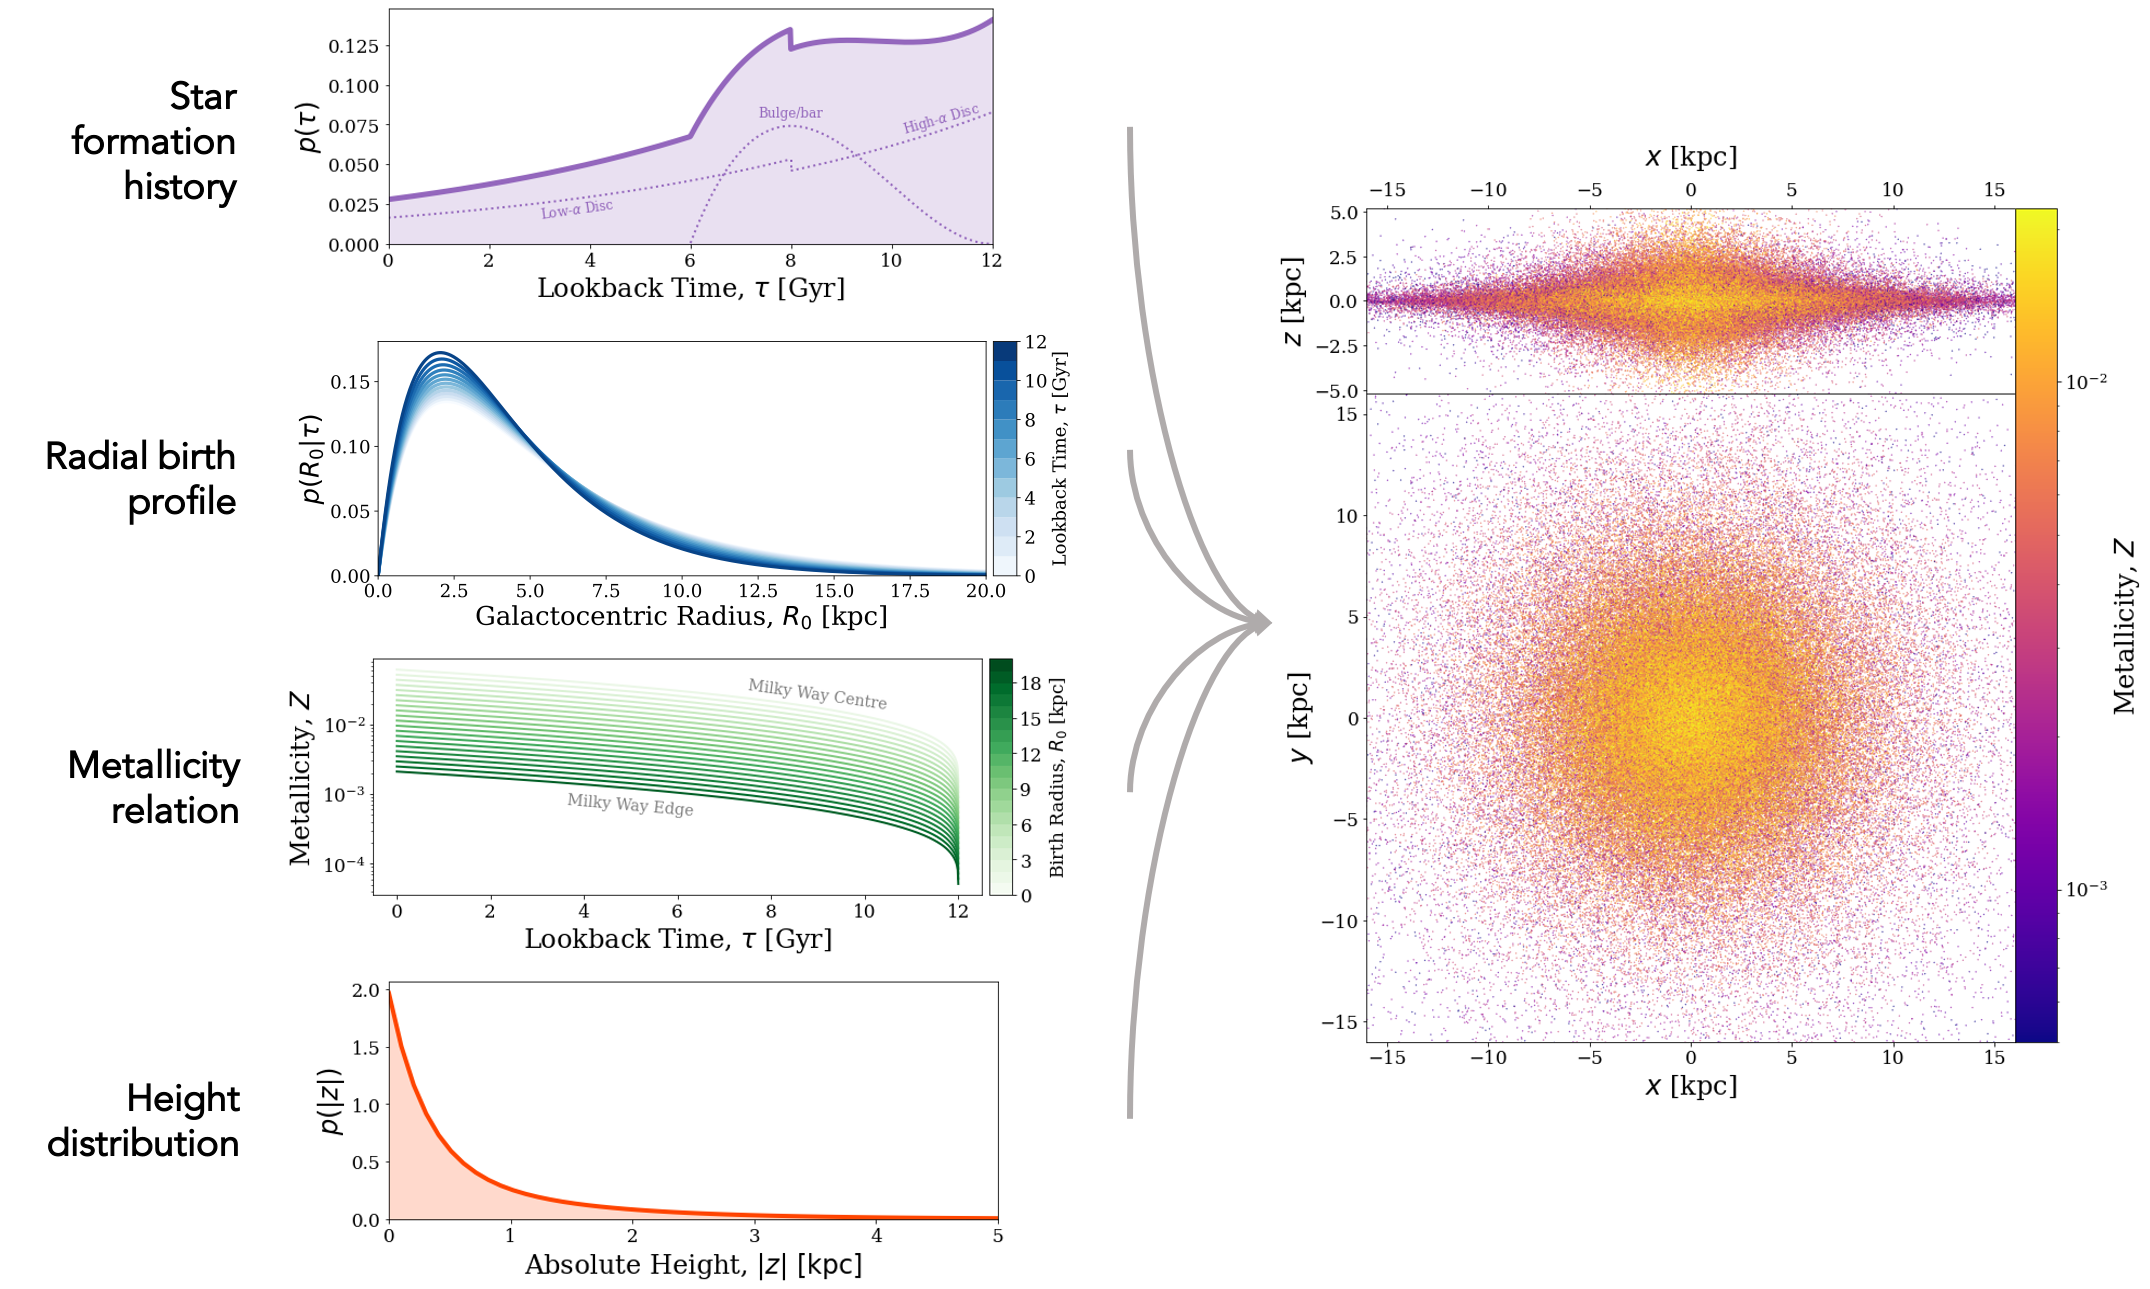
\includegraphics[width=\textwidth]{1_galaxy_diagram.png}
    \caption{A schematic illustrating how we create a mock Milky Way galaxy. The left panel illustrates the different model aspects: star formation history of 3 galactic components (individually shown in the dotted lines), spatial distribution at birth, age-metallicity-radius relation, and vertical distribution.
    On the right, we show an example instance of the Milky Way with $10^5$ binaries shown as points colour coded by metallicity. The top panel shows a side-on view and the bottom panel shows a face-on view.}
    \label{fig:galaxy_schematic}
\end{figure*}

Our model for the Milky Way accounts for the low-$\alpha$ disc, high-$\alpha$ disc and central bar/bulge. For each of these components, we use a separate star formation history, radial and vertical distribution, which we combine into a single model, weighting each component by its stellar mass. \citet{Licquia+2015} gives that the stellar mass of the bulge is $0.9 \times 10^{10} \unit{M_{\odot}}$ and the stellar mass of the disc is $5.2 \times 10^{10} \unit{M_\odot}$, which we split equally between the low- and high-$\alpha$ discs \citep[e.g.,][]{Snaith+2014}.

\textit{Star formation history:} 
We use an exponentially declining star formation history \citep{Frankel+2018} (a priori inspired by average the cosmic star formation history) for the combined low- and high-$\alpha$ disks, where the two disks transition at about 8 Gyr ago, and re-normalize the produced mass to be equal in each of the two components.
\begin{equation}\label{eq:thin_disc_tau}
    p(\tau) \propto \exp \qty(-\frac{(\tau_m - \tau)}{\tau_{\rm SFR}}),
\end{equation}
where $\tau$ is the lookback time (the amount of time elapsed between the binary's zero-age main sequence and today), $\tau_m = 12 \unit{Gyr}$ is the assumed age of the Milky Way and $\tau_{\rm SFR} = 6.8 \unit{Gyr}$ is the star formation timescale. 

The star formation history of the Milky Way bulge (which we assume here to be dominated by the central bar) has many uncertainties due to (1) sizeable age measurement uncertainties at large ages in observational studies, (2) complex selection processes affecting the observed age distributions, and (3) formation mechanisms still under debate. But the bulge was shown to contain stars with a range of 6-12 Gyr \citep[e.g.,][]{Bovy+2019}, where the younger tail of ages might come from the growth of the Galactic bar. To model the bulge age distribution more realistically than in previous studies (assuming an older bulge coming from a single starburst), we choose to adopt a star formation history using a $\beta(2,3)$ distribution, shifted and scaled such that stars are only formed in the range $[6, 12] \unit{Gyr}$

\textit{Radial distribution:} For each of the three components we employ the same single exponential distribution (but with different scale lengths)
\begin{equation}\label{eq:galaxy_R}
    p(R) = \exp(-\frac{R}{R_d}) \frac{R}{R_d^2},
\end{equation}
where $R$ is the Galactocentric radius and $R_d$ is the scale length of the component. For the low-$\alpha$ disc, we set $R_d = R_{\rm exp}(\tau)$, where $R_{\rm exp}(\tau)$ is the scale length presented in \citet[][Eq.~5]{Frankel+2018}
\begin{equation}
    R_{\rm exp}(\tau) = 4 \unit{kpc} \qty(1 - \alpha_{R_{\rm exp}} \qty(\frac{\tau}{8 \unit{Gyr}})),
\end{equation}
where $\alpha_{R_{\rm exp}} = 0.3$ is the inside-out growth parameter\footnote{In $R_{\rm exp}(\tau)$, we use 4 kpc instead of 3 kpc for the 0 Gyr exponential scale-length of the disc as NF finds that it provides a better fit to the original data}. This scale length accounts for the inside-out growth of the low-$\alpha$ disc and hence is age dependent. We assume $R_d = (1 / 0.43) \unit{kpc}$ for the high-$\alpha$ disc \citep[][Table~1]{Bovy+2016} and $R_d = 1.5 \unit{kpc}$ for the bar component \citep{Bovy+2019}.

\textit{Vertical distribution}: Similar to the radial distribution, we use the same single exponential distribution (but with different scale heights) for each component
\begin{equation}\label{eq:galaxy_z}
    p(\abs{z}) = \frac{1}{z_d} \exp\qty(-\frac{z}{z_d}),
\end{equation}
where $z$ is the height above the Galactic plane and $z_d$ is the scale height. We set $z_d = 0.3 \unit{kpc}$ for the low-$\alpha$ disc \citep{McMillan+2011} and $z_d = 0.95 \unit{kpc}$ for the high-$\alpha$ disc \citep{Bovy+2016}. 
\todo{Neige to Tom: for bar, I will think more for your bar scale-height, but the exact value should not change your results much since they will only slightly change the distance distribution of your sources, but not the rates nor the normalization.}
For the bulge, we set $z_d = 1.5 \unit{kpc}$ such that the probability of forming a star approaches zero at approximately the co-rotation radius of the Galactic bar/bulge \citep{Bovy+2019}. \todo{@Neige, did I justify the bulge/bar height correctly? A: The vertical distribution should not influence at which radius the bar should stop forming stars -- more later}

\textit{Metallicity-radius-time relation:} The relation is given by \citep[][Eq. 7]{Frankel+2018}
\begin{equation}\label{eq:galaxy_FeH}
    \begin{split}
        [{\rm Fe} / {\rm H}] (R, \tau) &= F_m + \nabla [{\rm Fe} / {\rm H}] R \\
        &- \qty(F_m + \nabla [{\rm Fe} / {\rm H}] R^{\rm now}_{[{\rm Fe} / {\rm H}] = 0} ) f(\tau),
    \end{split}
\end{equation}
where
\begin{equation}
    f(\tau) = \qty(1 - \frac{\tau}{\tau_m})^{\gamma_{[{\rm Fe} / {\rm H}]}},
\end{equation}
$F_m = -1 \unit{dex}$ is the metallicity of the gas at the center of the disc at $\tau = \tau_m$, $\nabla [{\rm Fe} / {\rm H}] = -0.075 \unit{kpc^{-1}}$ is the metallicity gradient, $R^{\rm now}_{[{\rm Fe} / {\rm H}] = 0} = 8.7 \unit{kpc}$ is the radius at which the present day metallicity is solar and $\gamma_{[{\rm Fe} / {\rm H}]} = 0.3$ set the time dependence of the chemical enrichment. We can convert this to the representation of metallicity that we use in this paper by applying \citep[e.g][]{Bertelli+1994}
\begin{equation}\label{eq:galaxy_FeH_to_Z}
    \log_{10} (Z) = 0.977 [{\rm Fe} / {\rm H}] + \log_{10}(Z_\odot).
\end{equation}

Although \citet{Frankel+2018} only fit this model for the low-$\alpha$ disc, we also use this metallicity-radius-time relation for the high-$\alpha$ disk and the bar, but focusing on the chemical tracks more representative to the inner disk and large ages. \citet{Sharma+2020} showed that using a simple continuous model for both the low- and high-$\alpha$ discs, the Milky Way abundance distributions could be well reproduced. Empirically, the chemical tracks in the [$\alpha$/Fe]-[Fe/H] plane of the stars in the bulge/bar follow the same track as those of the old stars in the Solar neighbourhood \citep[][Fig.~7,]{Bovy+2019}, which motivates our modelling choice to use the same metallicity-radius-time relation.

Fig.~\ref{fig:galaxy_schematic} shows the distributions and relations outlined in this section and also displays an example random galaxy drawn using this model.

\subsubsection{Combining population and galaxy synthesis}\label{sec:combining_pop_gal}

For each Milky Way instance, we randomly sample the following set of parameters
\begin{equation}
    \mathbf{g}_{{i}} = \{\tau, R, Z, z, \theta\}
\end{equation}
for $i = 1, 2, \dots, N_{\rm MW}$, where we set $N_{\rm MW} = 10^{5}$, $\tau, R, Z$ and $z$ are defined and sampled using the distribution functions specified in Section~\ref{sec:mw_model}, $\theta$ is the polar angle sampled uniformly on $[0, 2\pi)$ and $Z$ is the metallicity. Figure~\ref{fig:galaxy_schematic} shows an example of a random Milky Way instance created with these distributions. This shows how these distributions translate to positions in the Milky and illustrates the gradient in metallicity over radius.

We match each set of galaxy parameters $\mathbf{g}_{{i}}$, to a random set of binary parameters $\mathbf{b}_{{Z, i}}$, by randomly drawing a set of binary parameters from the closest metallicity bin to the metallicity in $\mathbf{g}_{{i}}$.

Each binary is likely to move from its birth orbit. Although all stars in the Galactic disc experience radial migration \citep{Sellwood+2002, Frankel+2018}, double compact objects generally experience stronger dynamical evolution as a result of the effects of both Blaauw kicks \citep{Blaauw+1961} and natal kicks \citep{Hobbs+2005}.

The magnitude of the systemic kicks are typically small compared to the initial circular velocity of a binary at each Galactocentric radius. Therefore, kicks will not significantly alter the overall distribution of their positions. Given this, and for the sake of computational efficiency, we do not account for the displacement due to systemic kicks in our analysis.

\subsection{Gravitational wave detection}\label{sec:gw_detection}
We use the Python package \href{https://legwork.readthedocs.io/en/latest/}{LEGWORK} to evolve binaries and calculate their LISA detectability. For a full derivation of the equations given below please see the LEGWORK release paper (Wagg et al. in prep) or \href{https://legwork.readthedocs.io/en/latest/notebooks/Derivations.html}{documentation}.

\subsubsection{Inspiral evolution}

Each binary loses orbital energy to gravitational waves throughout its lifetime. This causes the binary to shrink and circularise over time. In order to assess the detectability of a binary, we need to know its eccentricity and frequency at the time of the LISA mission. For each binary in our simulated Milky Way, we know that the time from DCO formation to today is $\tau - t_{\rm evolve}$ and that the initial eccentricity and semi-major axis are $e_{\rm DCO}$ and $a_{\rm DCO}$. We find the eccentricity of the binary at the start of the LISA mission, $e_{\rm LISA}$, by numerically integrating its time derivative \citep[][Eq. 5.13]{Peters+1964} given the initial conditions. This additionally can be converted to the semi-major axis at the start of LISA, $a_{\rm LISA} $\citep[][Eq. 5.11]{Peters+1964}, which in turn gives the orbital frequency, $f_{\rm orb, LISA}$, by Kepler's third law.

\subsubsection{Binary detectability}

We define a binary as detectable if its gravitational wave signal has a signal-to-noise ratio of greater than 7 \citep[e.g.][]{Breivik+2020, Korol+2020}. The sky-, polarisation- and orientation-averaged signal-to-noise ratio, $\rho$, of an inspiraling binary can be calculated with the following \citep[e.g.][]{Finn+2000}
\begin{equation}\label{eq:snr}
    \rho^2 = \sum_{n=1}^{\infty} \int_{f_{n, i}}^{f_{n, f}} \frac{h_{c, n}^{2}}{f_{n}^{2} S_{\rm n}\left(f_{n}\right)} \dd{f_n},
\end{equation}
where $n$ is a harmonic of the gravitational wave signal, $f_n = n \cdot f_{\rm orb}$ is the frequency of the $n^{\rm th}$ harmonic of the gravitational wave signal, $f_{\rm orb}$ is the orbital frequency, $S_{\rm n}(f_n)$ is the LISA sensitivity curve at frequency $f_n$ \citep[e.g.][]{Robson+2019} and $h_{c,n}$ is the characteristic strain of the $n^{\rm th}$ harmonic, given by \citep[e.g.][]{Barack+2004}
\begin{equation}\label{eq:charstrain}
    h^2_{c,n} = \frac{2^{5/3}}{3 \pi^{4/3}} \frac{(G \mathcal{M}_c)^{5/3}}{c^3 D_L^2} \frac{1}{f_{\rm orb}^{1/3}} \frac{g(n,e)}{n F(e)},
\end{equation}
where $D_L$ is the luminosity distance to the source, $f_{\rm orb}$ is the orbital frequency, $g(n, e)$ and $F(e)$ are given in \citet{Peters+1963} and $\mathcal{M}_c$ is the chirp mass, defined as
\begin{equation}\label{eq:chirp_mass}
    \mathcal{M}_c = \frac{(m_1 m_2)^{3/5}}{(m_1 + m_2)^{1/5}}.
\end{equation}

We use LEGWORK to calculate the signal-to-noise ratio for each binary and the package ensures that enough harmonics are computed for each binary such that the error on the gravitational wave luminosity remains below 1\%.

\subsubsection{Detection rate calculation}
For any one instance of the Milky Way, we calculate the detection rate 

For each physics variation model, we compute the total number of merging DCOs in the Milky Way today, $N_{\rm MW}$, based on the COMPAS simulation. This takes into account the true mass and IMF of the Milky Way since our simulations each have a slightly smaller galaxy size and only sample from massive stars rather than the full IMF. For a more in-depth discussion of this process see Appendix~\ref{app:rate_normalisation}.

We determine the fraction of binaries that are detectable in each Milky Way instance by summing the adaptive importance sampling weights of the binaries that have an SNR greater than 7 and dividing by the total weights in the simulation. We multiply this fraction by the total number in the Milky Way to find a detection rate.
\begin{equation}
    N_{\rm detect} = \frac{\sum_{i = 0}^{N_{\rm detect}} w_i}{\sum_{i = 0}^{N_{\rm DCO}} w_i} \cdot N_{\rm MW}
\end{equation}
We calculate the detection rate by Monte Carlo sampling 2500 Milky Way instances (each containing 100,000 DCOs) for each DCO type and every physics variation in order to obtain values for the uncertainty on the expected detection rate.

\section{Results} \label{sec:results}
In this section we present our main results for the detectable LISA DCO population in our fiducial model. We find that on average, a 4-year LISA mission will detect about \BHBHFourYear{} BHBHs, \BHNSFourYear{} BHNSs and \NSNSFourYear{} NSNSs (c.f.\ Table~\ref{tab:detection_rates}). We first show the distribution of the sources together with the sensitivity curve in Section~\ref{sec:dcos_on_sc}, before exploring the parameter distributions for detectable sources in Section~\ref{sec:fiducial_distributions} and the measurement uncertainties in Section.~\ref{sec:measurement_uncertainties}.

\subsection{Distribution on the sensitivity curve}\label{sec:dcos_on_sc}

\begin{figure*}[p]
    \centering
    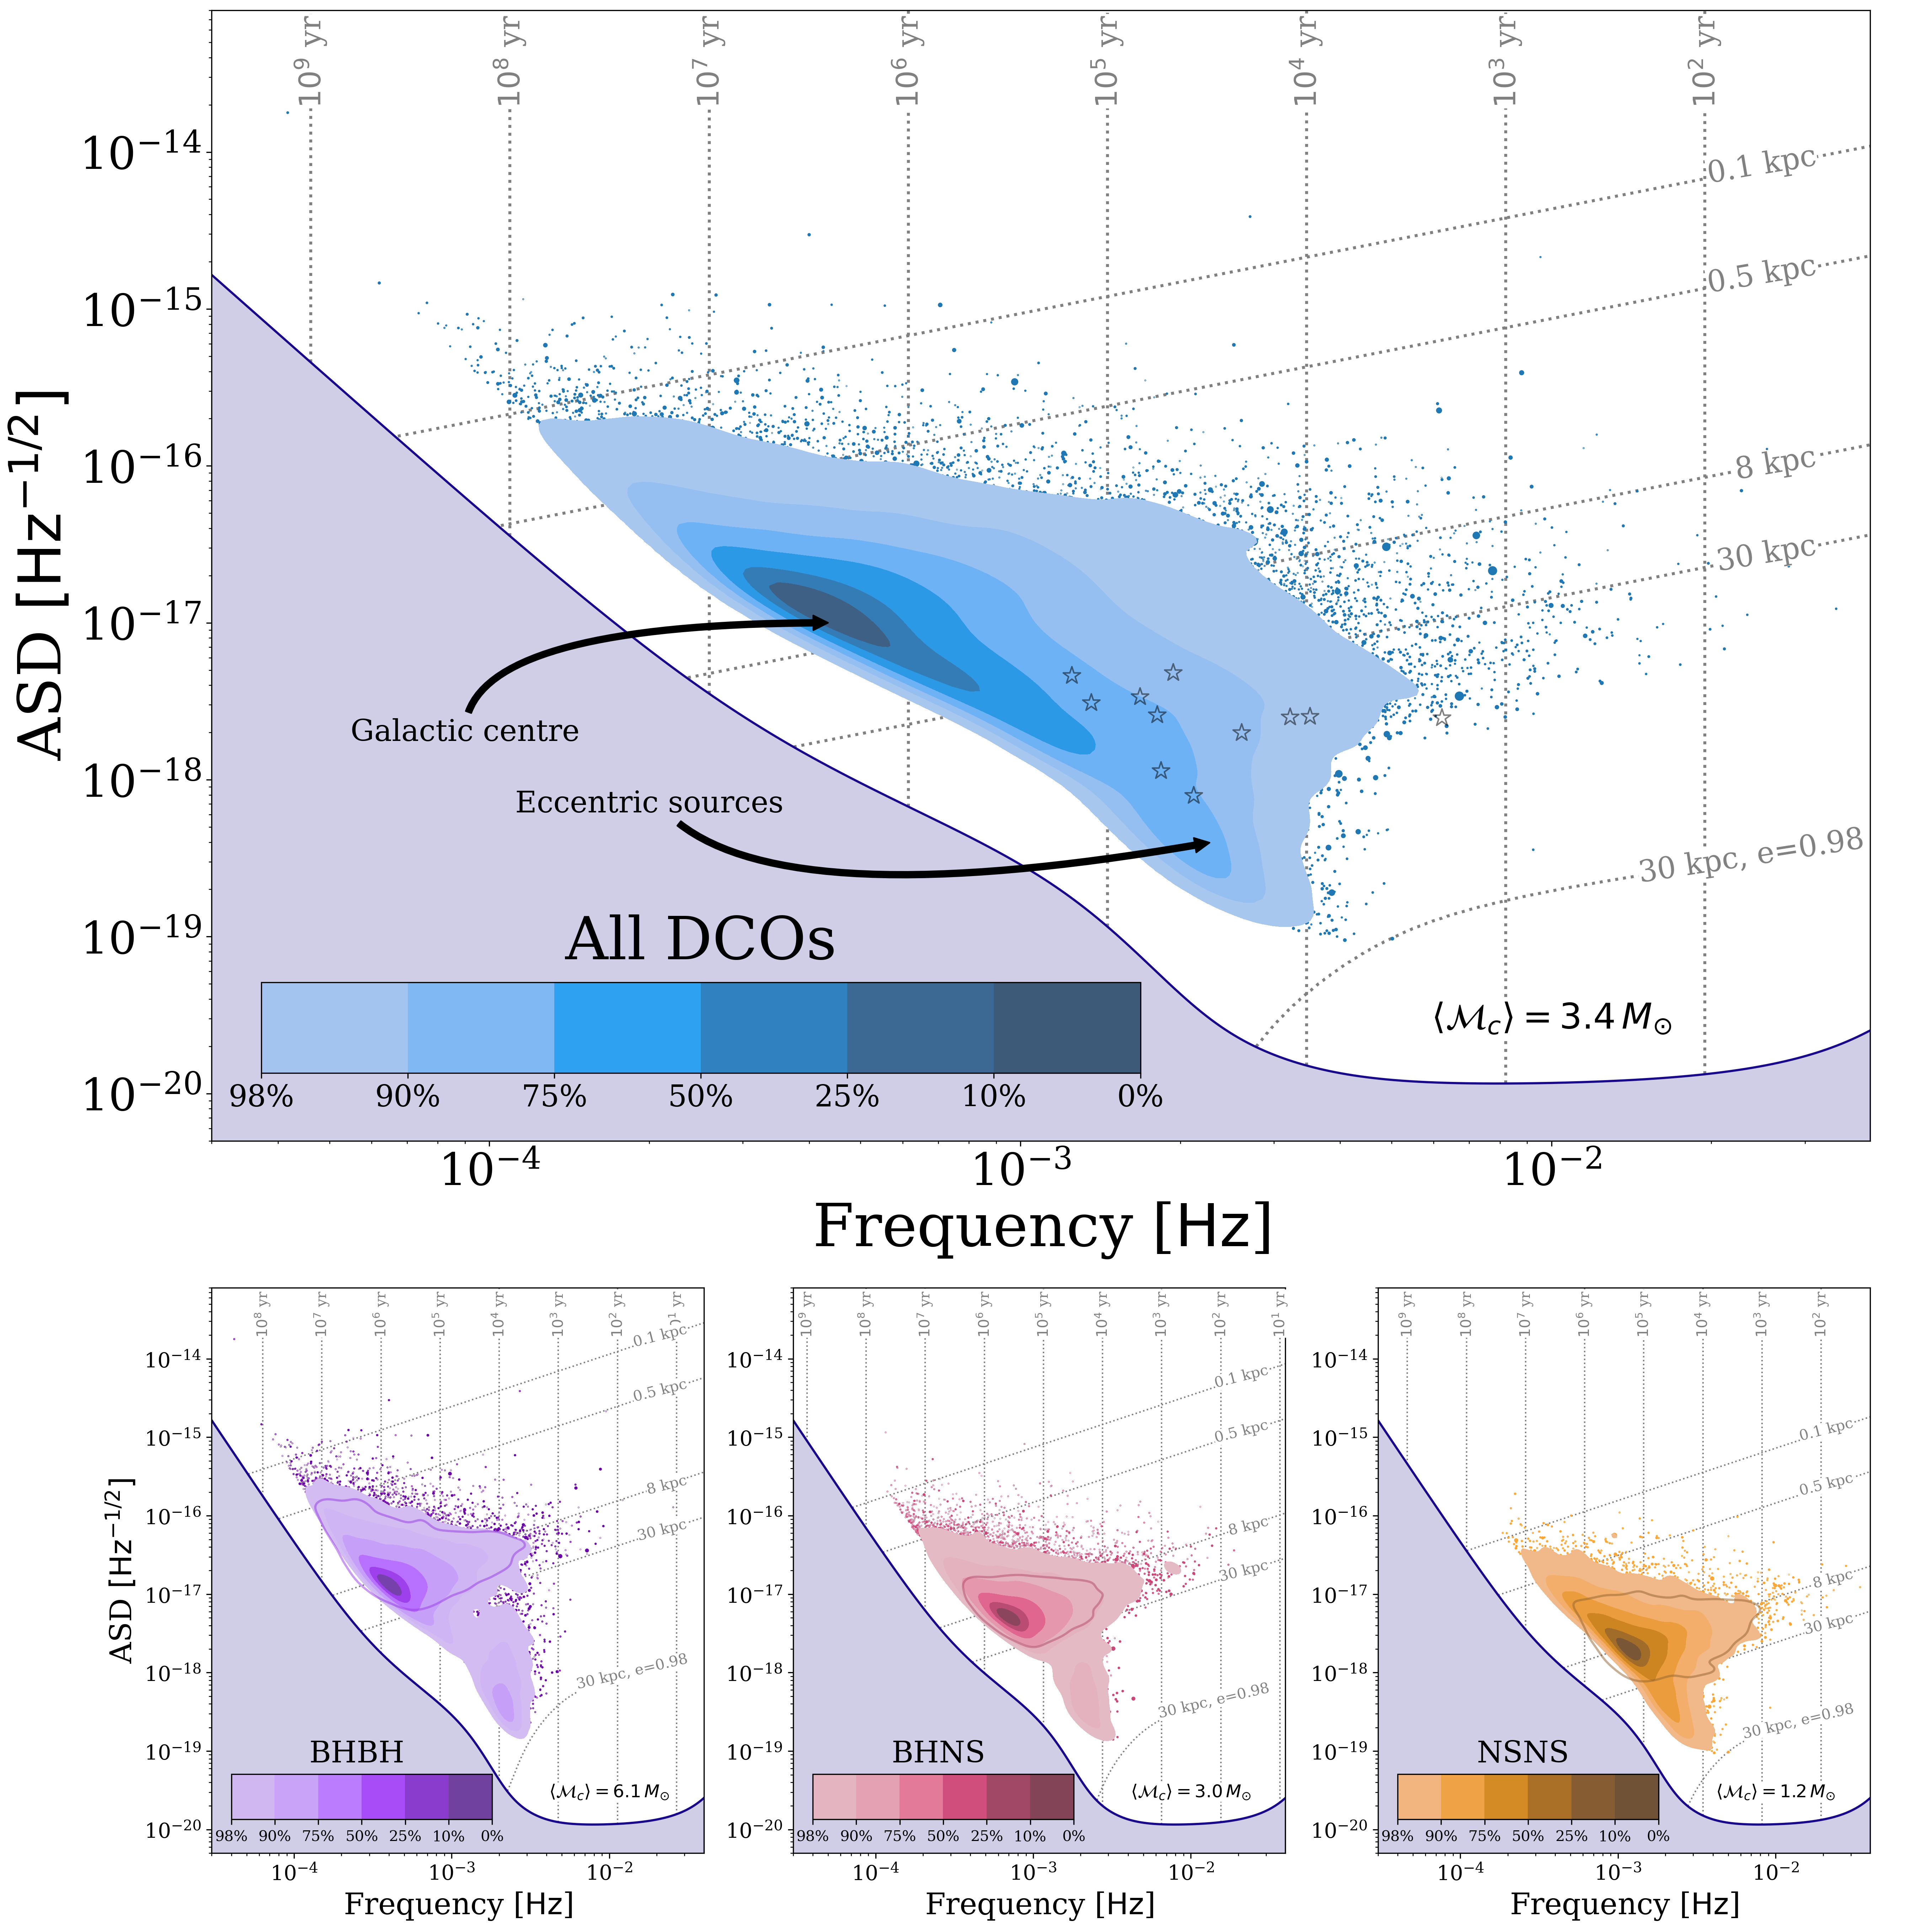
\includegraphics[width=\textwidth]{2_dcos_on_sc.png}
    \caption{Density distribution of detectable BHBH, BHNS and NSNS binaries are shown together with the LISA sensitivity curve. In the top panel we show all systems with the LISA verification binaries over plotted (star symbols, \citealp{Kupfer+2018}). In the bottom panels we separate by type. Contours show the percentage of the population enclosed. The remaining 2\% of the population is shown as dots with a size that scales with the sampling weight. For reference we show lines where a circular binary of average chirp mass $\avg{\mathcal{M}_c}$ would reside for a given remaining inspiral time (vertical lines) and distance (diagonal line). To highlight the role of eccentricity we further show the signal expected for an eccentric binary at 30 kpc. The coloured line in the bottom panels shows a contour that encloses 90\% of the population that is circular. See Sec.~\ref{sec:dcos_on_sc} for a discussion.}
    \label{fig:dcos_on_sc}
\end{figure*}

We show the expected distribution of detectable DCOs together with the LISA sensitivity curve in Figure~\ref{fig:dcos_on_sc}. This shows that the detectable population of these DCOs is concentrated at comparatively lower frequencies than the LISA verification binaries (shown as stars in the top panel). This is expected since producing the same SNR as a BHBH, BHNS or NSNS with a relatively lower mass (circular) WDWD requires a higher frequency. This finding is in agreement with \citet{Sesana+2020} and as noted in that work, this could possibly be used to distinguish more massive DCOs from WDWDs probabilistically. There are several other notable features in these distributions. To understand these we overplot reference lines indicating where a circular binary with the average chirp mass ($\avg{\mathcal{M}_c}$, annotated in each panel) would reside for a given remaining inspiral time (vertical lines) and a given distance (diagonal lines).

Firstly, we note that the peak of the density distribution coincides with the centre of the Milky Way as expected, since binaries are most likely to be formed towards the centre of the Galaxy. Additionally, we expect that if a population is entirely circular, it should be bounded approximately between the $0.1$--$30 \unit{kpc}$ lines, roughly the minimum and maximum distance to a source in the Milky Way. From inspection of the bottom panels with each individual DCO type we see that this is the true for a large fraction of the population. However, there is a distinct subpopulation of binaries that extend downwards, especially around $2 \unit{mHz}$. This offshoot is composed of eccentric binaries for which the circular distance contours do not apply. For illustrative purposes, we plot the 90\% contour of only the \textit{circular} sources in our sample over the density distribution in each of the bottom panels and this subsample is indeed bounded by $0.1$--$30 \unit{kpc}$ the distance lines. We also plot a line of constant distance at $30 \unit{kpc}$ for an eccentric binary with $e = 0.98$ to show the different limit for eccentric sources. To further illustrate this point, we show the same plot but with each point coloured by its eccentricity in Fig.~\ref{fig:dcos_on_sc_ecc_col}. Overall, we can see that eccentric sources tend to be located on a slightly different location on the sensitivity curve and so this could perhaps be used help in identifying them.

We plot vertical lines that give the inspiral time for a circular binary with the average chirp mass (annotated in each panel). From these lines we can understand the trend of the density distribution decreasing with increasing frequency. Sources with higher frequencies have shorter inspiral times and thus DCOs will spend less time in these regimes, meaning that more sources are detected at lower frequencies. Note that these inspiral time lines should only be used as guidelines for the population as a whole, as the inspiral time of each individual source will be a function of its mass and eccentricity. It is also evident for each DCO source that the tail of the high frequency sources is more numerous near to the Galactic centre than at short distances. This is simply because there are more sources in the galactic centre and so the chances of `catching' a binary at high frequency are better.

\subsection{Properties of the detectable systems}\label{sec:fiducial_distributions}

In Figure~\ref{fig:fiducial_pdf_distributions}, we show the distribution of the individual parameters of the population of detectable binaries and discuss the various features in the following sections.

\subsubsection{Orbital Frequency}
The orbital frequency distributions for BHBHs, BHNSs and NSNSs peak at progressively increasing frequencies. This is because a higher mass DCO at the same distance and eccentricity requires a lower frequency to produce the same signal-to-noise ratio and thus be detected. The BHBH distribution has a tail that extends to $8 \times 10^{-6} \unit{Hz}$, which is comprised of highly eccentric binaries. These systems are still detectable by LISA as the high eccentricity means that the majority of the GW signal is emitted at higher harmonics at higher frequencies that are located in the LISA band. Similar tails are not as prevalent for BHNSs and NSNSs as they do not have as many eccentric binaries.

\begin{figure*}[t]
    \centering
    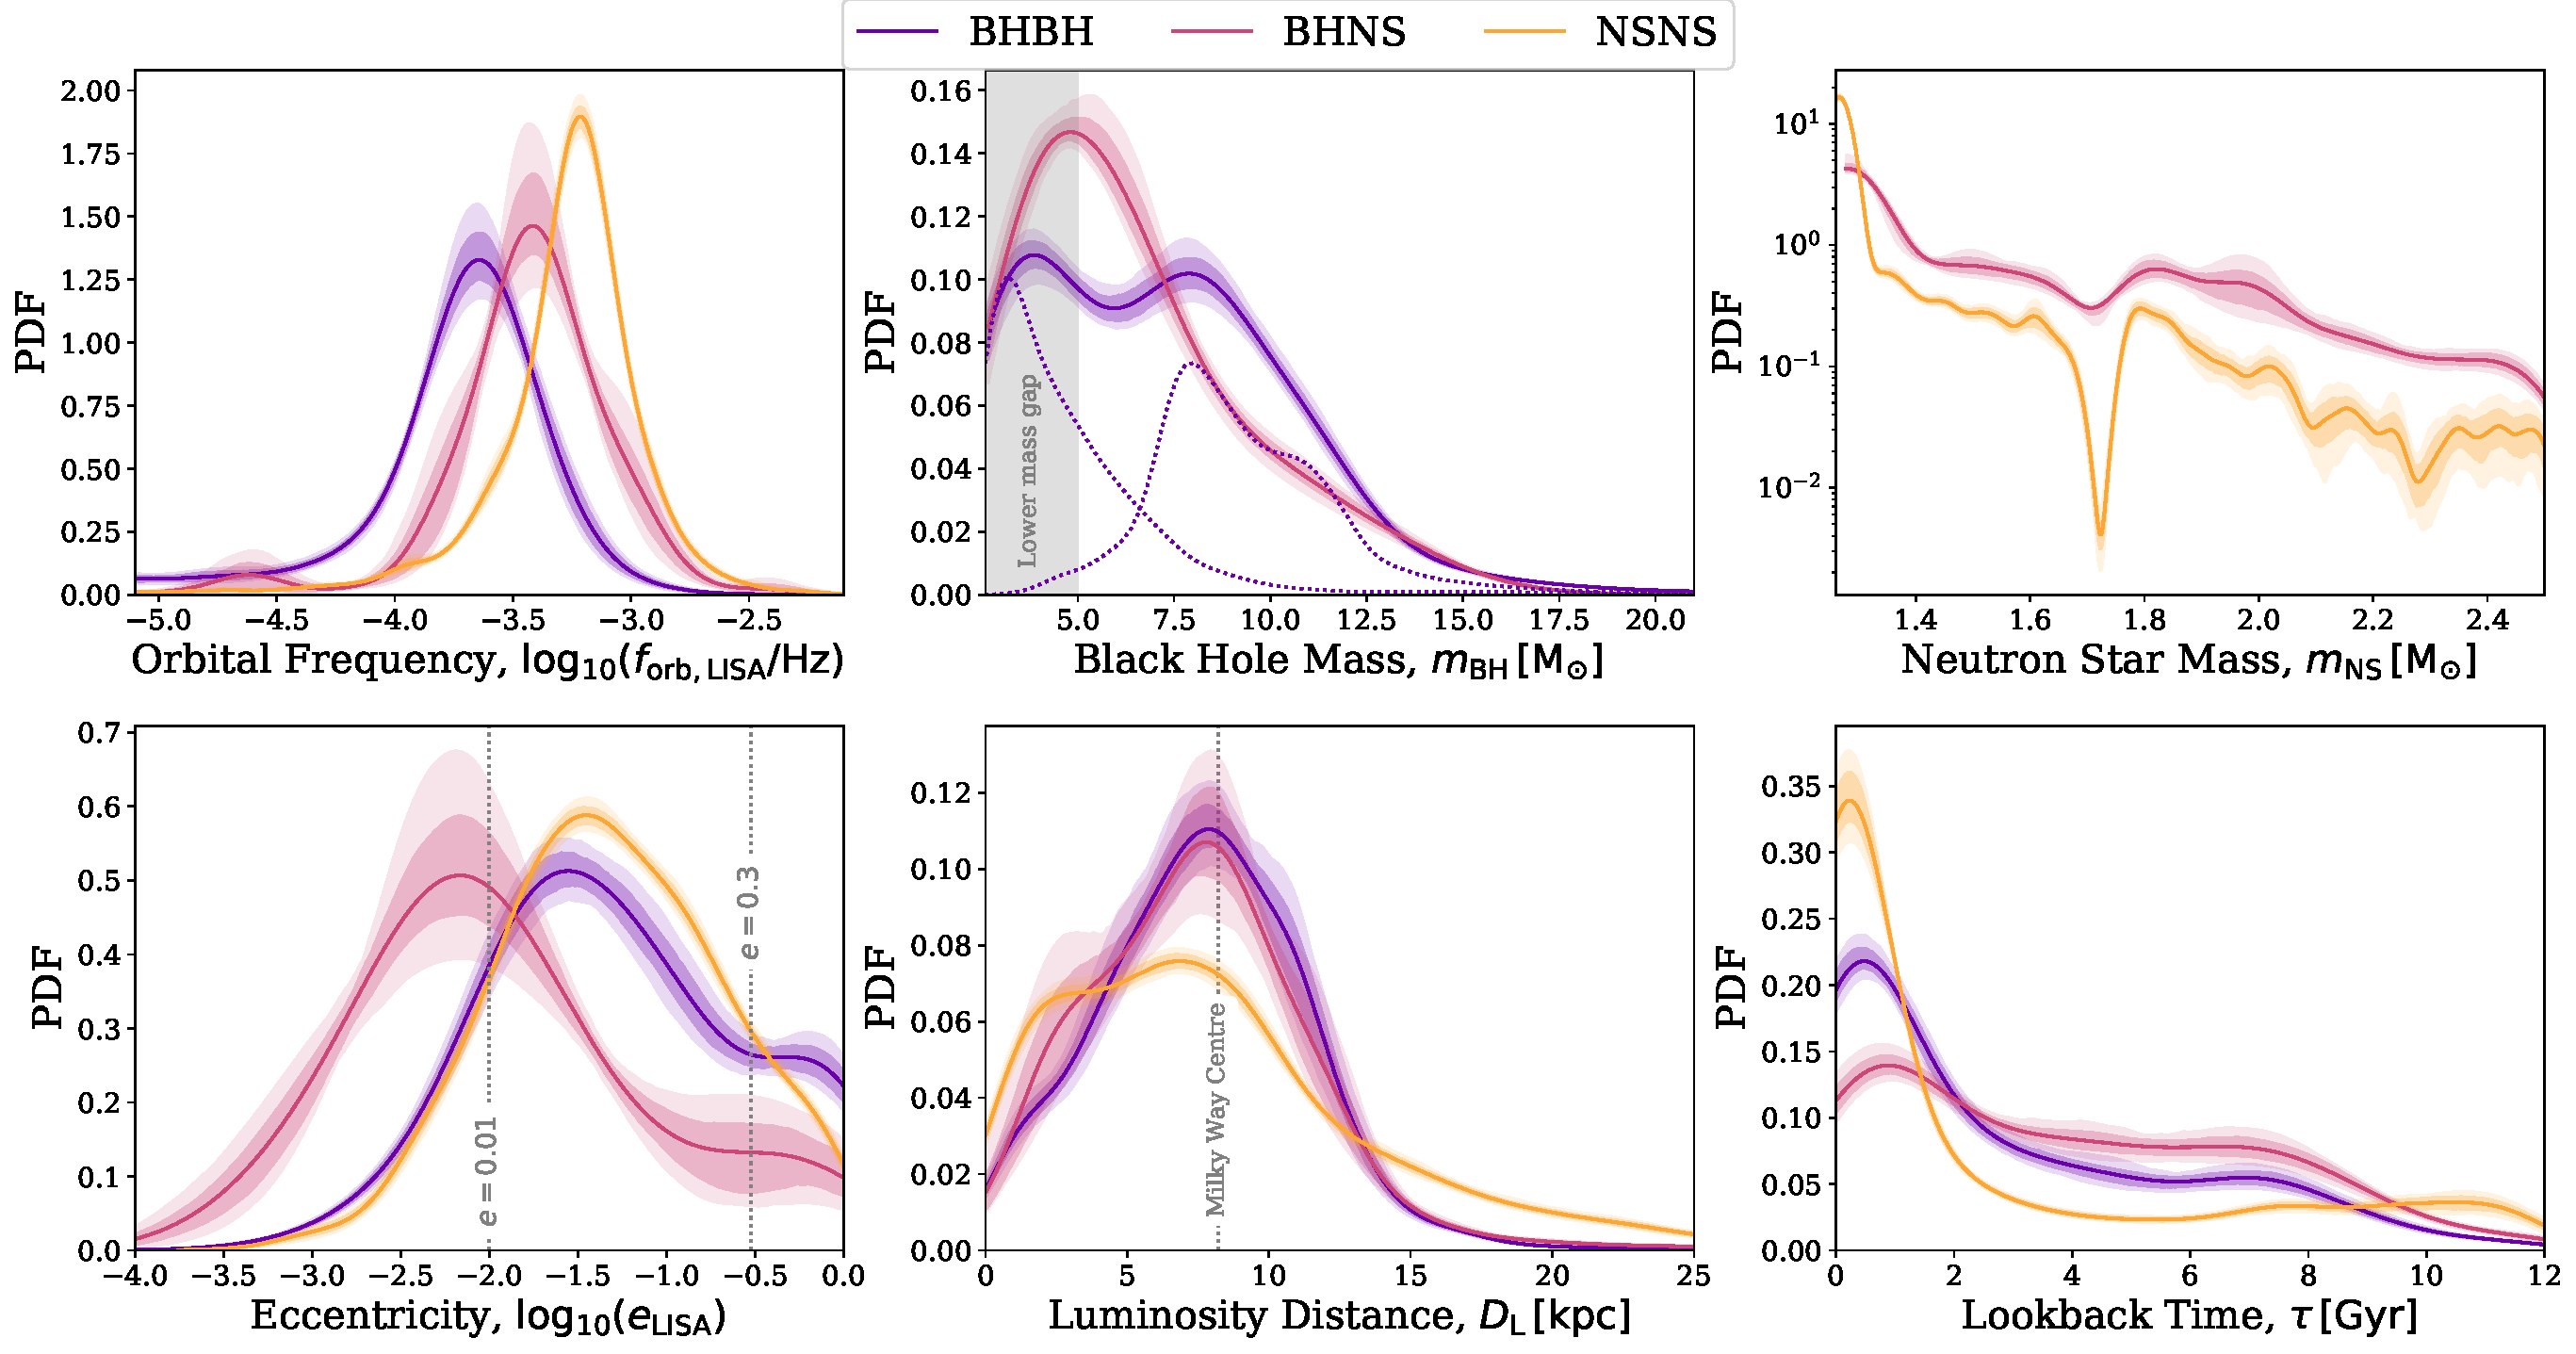
\includegraphics[width=\textwidth]{4_detectable_properties_4yr.pdf}
    \caption{Properties of detectable systems for a 4-year LISA mission in our fiducial model. Each panel shows a kernel density estimator for a single property, coloured by DCO type. The shaded areas show the 1- and 2-$\sigma$ uncertainties (obtained via bootstrapping). The dotted lines in the black hole mass panel show the individual primary and secondary mass distributions. See Sec.~\ref{sec:fiducial_distributions} for a discussion.}
    \label{fig:fiducial_pdf_distributions}
\end{figure*}

\subsubsection{Black Hole Mass}
For both the BHBHs and BHNSs, the black hole mass distribution extends to relatively low masses, with $\BHBHmBHBelowEleven{}$ and $\BHNSmBHBelowEleven{}$ respectively below $11 \unit{M_{\odot}}$. Unlike ground-based detectors, LISA is not biased to higher masses and so the mass distribution more closely follows the IMF. In addition, at the high metallicities in the Milky Way, stellar winds are much stronger and strip away much of the stellar mass before BH formation, resulting the less massive black holes. The mass distribution extends down to $2.5 \unit{M_{\odot}}$, our fiducial maximum neutron star mass. Since the \citet{Fryer+2012} \textit{delayed} remnant mass prescription (applied in this work) does not produce a mass gap between neutron stars and black holes. Indeed we expect $\BHBHLowerMassGap{}$ and $\BHNSLowerMassGap{}$ of detected BHBH and BHNS systems to contain a black hole in the lower mass gap. Therefore, LISA could help to confirm or rule out the existence of the lower mass gap.

The bimodality of the BHBH distribution is a result of unequal mass ratios. The two peaks are from the primary and secondary black hole masses, which peak around $8 \unit{M_{\odot}}$ and $3.5 \unit{M_{\odot}}$ respectively. We show these individual distributions as dotted curves below the main BHBH distribution.

\subsubsection{Mass Ratio}
The mass ratio distribution for each DCO type is relatively distinct from the others. The majority of NSNSs have a mass ratio close to unity, with $\NSNSqAbovePointEight{}$ of systems having $q > 0.8$. The reason for the concentration around equal masses is that most NSs are formed either through electron-capture supernovae or from low mass stars. We set the remnant mass for any system formed through ECSN to $1.26 \unit{M_{\odot}}$ (see Sec.~\ref{sec:fiducial_physics}). The remnant mass prescription that we use gives a fixed fallback mass for any star with a CO core mass less than $2.5 \unit{M_\odot}$, such that many NSs are given the identical mass of $1.278 \unit{M_\odot}$ in the \textit{delayed} prescription \citep[see][Eq.~19]{Fryer+2012}. This means that many NSs are formed with equal masses and hence we see a mass ratio distribution peaked around unity.

In contrast, only $\BHBHqAbovePointEight{}$ of detectable BHBHs are formed with $q > 0.8$ and distribution peaks around $q = 0.4$. The reasoning for these unequal mass ratio systems is as follows: in order to produce a BHBH, most formation channels require at least the first mass transfer to be stable. This stability is strongly dependent on the mass ratio such that equal mass ratios (at the moment of mass transfer) are preferred for creating BHBHs. Yet, since stellar winds are so strong at high metallicity, and even stronger for more massive stars, the primary star will experience significant mass loss and so an initially \textit{unequal} mass ratio is preferred so that the masses are more balanced at the first instance of mass transfer. Since mass transfer occurs after the end of the main sequence for most of our BHBHs, the star will have a well defined core and these core masses, which go on to form BHs, will reflect the initially unequal mass ratios.

We find that detectable BHNSs have even more unequal mass ratios, such that the distribution is almost entire disjoint from that of NSNSs. Moreover, the mass ratio distribution is bimodal, where the two peaks arise from two distinct formation scenarios. Around two thirds of detectable BHNSs experience at least one common envelope event, whilst the last third are formed through only stable mass transfer. The first peak at $q = 0.18$ is from systems that experience at least one CE and occurs at the expected mass ratio, which approximately follows the mean BH mass ($\sim 6.5 \unit{M_\odot}$) and NS mass ($\sim 1.2 \unit{M_\odot}$). Yet we also see a second peak at higher mass ratios around $q = 0.34$, which arise from the fraction of the population that underwent only stable mass transfer. The stability of mass transfer is strongly dependent on the mass ratio and thus these systems have a bias for more equal mass ratio systems, leading to a peak at higher $q$.

\subsubsection{Eccentricity}
The eccentricity distributions show that detectable BHBHs are most likely to be highly eccentric of the three DCOs. This may seem counter-intuitive since neutron stars receive stronger natal kicks, which cause the orbit to become eccentric. However, these stronger kicks often result in disrupted or too-wide binaries in the more weakly bound NSNSs. In contrast, BHBHs can receive strong kicks that impart high eccentricity without disrupting and thus tend to be more eccentric. This effect is compounded by the fact that we can see BHBHs at lower orbital frequencies, meaning that they have not had as much time to circularise and so still have significant eccentricity by the time of the LISA mission.

An eccentricity of $e = 0.01$ is the lower bound on the measurable eccentricity with LISA proposed by \citet{Nishizawa+2016}. We find that a significant fraction of DCOs ($\BHBHNotCirc{}$ of BHBHs, $\BHNSNotCirc{}$ of BHNSs and $\NSNSNotCirc{}$ of NSNSs) exceed this bound. This is in contrast to several previous work that assume all DCOs are circular once they reach the LISA mission \citep[e.g.][]{Lamberts+2018, Sesana+2020}. Moreover, we find that $\BHBHHighlyEccentric{}$, $\BHNSHighlyEccentric{}$ and $\NSNSHighlyEccentric{}$ of BHBHs, BHNSs and NSNSs respectively have $e > 0.3$. At this eccentricity the majority of the gravitational wave power is emitted in higher harmonics above the orbital frequency and thus the signal would appear at higher frequencies in LISA.

\subsubsection{Time since formation}
The progenitors of Galactic DCOs in our sample are formed throughout the history of the Milky Way, with more formed at earlier times (see Fig.~\ref{fig:galaxy_schematic}). In contrast, we find that the \textit{detectable} systems are primarily formed recently, with the majority formed in the past $2 \unit{Gyr}$, in addition to a tail of systems out to earlier times.

The peak at recent times is due to the fact that most binaries in our sample are formed with merger times on the order of a couple of Gyr (since most form through a common envelope phase that significantly tightens the binary). For a binary to be in the LISA band and detectable it must be near the end of its inspiral and so LISA will be most sensitive to sources that were formed a couple of Gyr ago.

The peak is sharpest for NSNSs as they have the highest orbital frequencies and largest fraction of eccentric system, which result in shorter inspiral times and therefore later formation times. Conversely, the peak is less prominent for BHNSs as they are the most circular, have moderate orbital frequencies and masses.

\subsubsection{Time until merger}
The final panel of Fig.~\ref{fig:fiducial_pdf_distributions} shows the remaining time until merger for each of the DCO types at the start of LISA mission. The distributions are strikingly similar and peak with merger times of around a Myr.

The merger time is a function of the mass, frequency and eccentricity of the sources, such that more massive, higher frequency and more eccentric sources merge faster \citep[][Eq.~5.14]{Peters+1964}. So, despite the fact that each DCO type often has higher values in any one of these properties, the convolution of all three tends to negate the differences. For example, NSNSs have the highest orbital frequencies and are mildly eccentric whilst BHNSs have moderate orbital frequencies and are more circular. However, BHNSs are more massive in general and so the overall merger times are distributed very similarly for both DCO types.

\subsection{Distribution in the Milky Way}\label{sec:mw_detectable_distribution}
In the first panel of Fig.~\ref{fig:detectable_distance_dist} we show the distribution of the luminosity distance of detectable systems. Each DCO's luminosity distance distribution peaks around $8 \unit{kpc}$ since this is the distance to the centre of the Milky Way and thus the most dense location of DCOs. There is a bias in each distribution for systems at lower distances since closer binaries are easier to detect. This bias is most prominent for the NSNS distribution since, on average, their lower relative masses require a smaller distance in order to be detected.

However, more surprisingly, we also see that the NSNS distribution extends to higher distances than the other DCOs. The reason for this is that the NSNS population has the highest fraction of ``mildly'' eccentric systems ($0.01 < e < 0.3$). The BHNS population has a much higher fraction of effectively circular systems ($e < 0.01$), which emit weaker gravitational wave compared to equivalent eccentric systems. Therefore, despite their relatively higher masses, the maximum distance at which a source is detectable is generally lower than the eccentric NSNSs and hence the distribution tends to zero at smaller distances. Conversely, the BHBH population has a higher fraction of \textit{high} eccentricity systems $e > 0.3$. Although one may naively expect that this would result in stronger signals (and so further distances), for a system to have these high eccentricities in LISA, it must still be early in its evolution and thus have a low orbital frequencies. The result of this is that high eccentricity systems tend to have lower SNRs and so cannot be detected at large distances. Overall we see that the eccentricity distribution of NSNSs occupies a ``sweet spot'' where the gravitational wave power is increased compared to circular systems, but it isn't too high that the frequency is significantly impacted. This means that NSNSs can be seen out to the largest distances of the three DCO types.

\todo{There will also be a little bit more text to explain the example distribution over galaxies in the lower panel -- will make properly once Floor combines the latest fiducial simulation data (this plot is sampling uniformly rather than based on the distribution)}

\begin{figure}[thb]
    \centering
    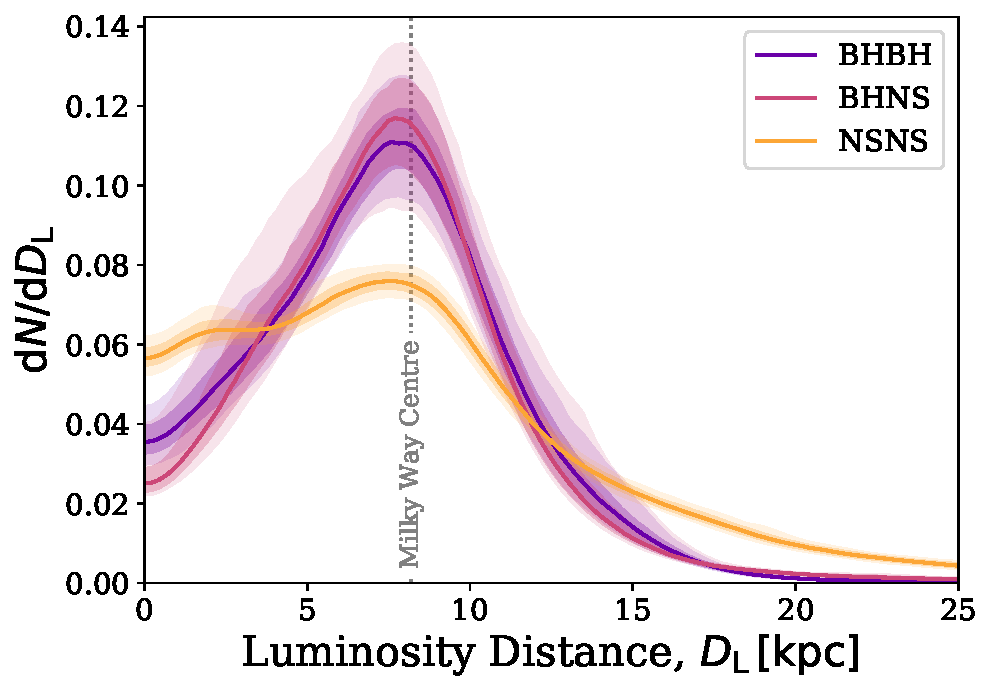
\includegraphics[width=\columnwidth]{detectable_distance_distribution_4yr.pdf}
    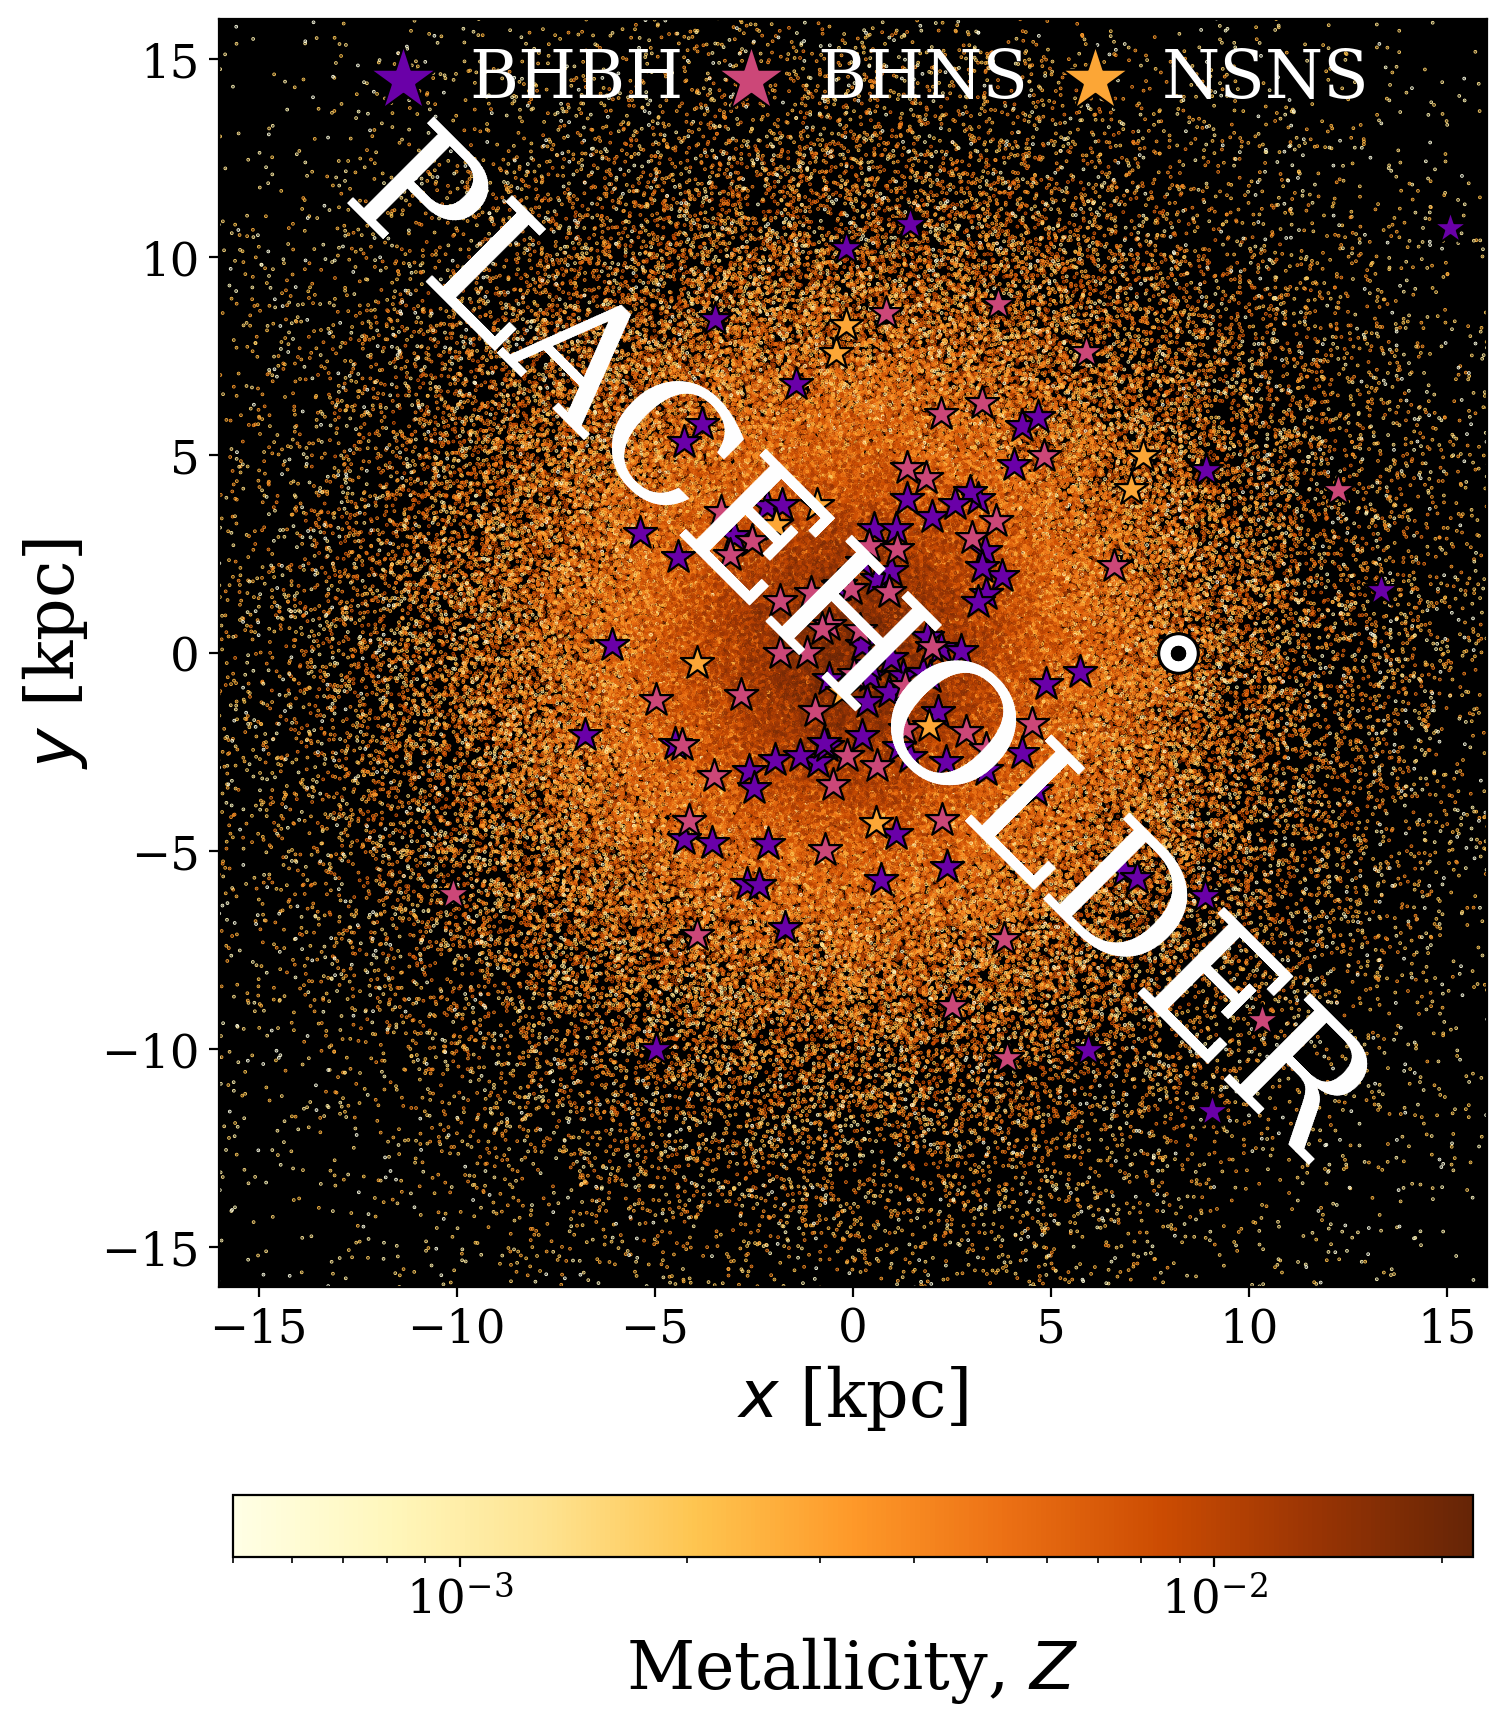
\includegraphics[width=\columnwidth]{sources_on_mw.png}
    \caption{\textbf{Top:} As Figure~\ref{fig:fiducial_pdf_distributions}, but for the luminosity distance. \textbf{Bottom:} A face-on view of an example Milky Way galaxy, where each point is coloured by its metallicity. The large $\odot$ shows the position of the Sun. Stars represent a typical example of the detectable systems in a 4-year LISA mission. \todo{make proper plot, maybe separate panels for different types (hard to arange then though), thoughts on black background?}}
    \label{fig:detectable_distance_dist}
\end{figure}

\subsection{Measurement Uncertainties}\label{sec:measurement_uncertainties}
Although it is useful to investigate the underlying parameters of the detectable population, it is also important to consider what LISA will actually \textit{measure} during a detection.

\subsubsection{Chirp mass uncertainty}

The chirp mass uncertainty is important for identifying the source of a GW signal. It is calculated using the uncertainty on the orbital frequency, the time derivative of the orbital frequency and the eccentricity. This is because the chirp mass can be written as
\begin{equation}
    \mathcal{M}_c = \frac{c^3}{G} \left( \frac{5 \pi}{48 n} \frac{\dot{f}_{n}}{F(e)} \right)^{3/5} \frac{1}{(2 \pi f_{\rm orb})^{11/5}},
\end{equation}
where $f_{\rm orb}$ is the orbital frequency, $\mathcal{M}_{c}$ is the chirp mass (defined in Eq.~\ref{eq:chirp_mass}), $e$ is the eccentricity and
\begin{equation}
    F(e) = \frac{1 + \frac{73}{24} e^2 + \frac{37}{96} e^4}{(1 - e^2)^{7/2}},
\end{equation}
is the enhancement factor of gravitational wave emission for an eccentric binary over an otherwise identical circular binary \citep[][Eq.~17]{Peters+1963}. Therefore the chirp mass uncertainty is
\begin{equation}\label{eq:chirp_mass_uncertainty}
    \qty( \frac{\Delta \mathcal{M}_c}{\mathcal{M}_c} )^2 = \left( \frac{11}{5} \frac{\Delta f_{\rm orb}}{f_{\rm orb}} \right)^2 + \left( \frac{3}{5} \frac{\Delta \dot{f}_{\rm dom}}{\dot{f}_{\rm dom}} \right)^2 + \left( \frac{3}{5} \frac{\Delta F(e)}{F(e)} \right)^2,
\end{equation}
where $f_{\rm dom}$ is the harmonic frequency with the strongest SNR ($f_{\rm dom} = n_{\rm dom} f_{\rm orb}$ and $n_{\rm dom} = 2$ for circular binaries) as this will provide the best measurement.

We calculate the frequency uncertainties using \citet{Takahashi+2002}, such that
\begin{align}\label{eq:f_orb_unc}
    \frac{\Delta f_{\rm orb}}{f_{\rm orb}} &= 4 \sqrt{3} \cdot \frac{1}{\rho} \frac{1}{T_{\rm obs}} \frac{1}{f_{\rm orb}}, \\
    \frac{\Delta \dot{f}_{\rm dom}}{\dot{f}_{\rm dom}} &= 6 \sqrt{5} \cdot \frac{1}{\rho} \left(\frac{1}{T_{\rm obs}} \right)^2 \frac{1}{\dot{f}_{\rm dom}},
\end{align}
where $\rho$ is the signal-to-noise ratio and $T_{\rm obs}$ is the LISA mission length. We calculate the eccentricity certainty, $\Delta e$, following the methods of \citet{Lau+2020} and \citet{Korol+2021}, which use the relative SNRs of different harmonics to work out the eccentricity. We propagate this uncertainty such that
\begin{equation}
    \frac{\Delta F(e)}{F(e)} = \Delta e \cdot \frac{(1256 + 1608 e^2 + 111 e^4) e}{96 + 196 e^2 - 255 e^4 - 37 e^6}.
\end{equation}

We use Eq.~\ref{eq:chirp_mass_uncertainty} to calculate the chirp mass uncertainty for each DCO in our sample and plot it in Fig.~\ref{fig:m_c_unc}. We find that approximately $\BHBHChirpMassMeasureable{}$ BHBHs, $\BHNSChirpMassMeasureable{}$ BHNSs and $\NSNSChirpMassMeasureable{}$ NSNSs have measurable chirp masses (as indicated by the shaded region). This uncertainty is generally dominated by the uncertainty on the time derivative of the frequency, since most of the binaries are too early in their inspiral for LISA to measure a strong chirp.

\begin{figure}[ht]
    \centering
    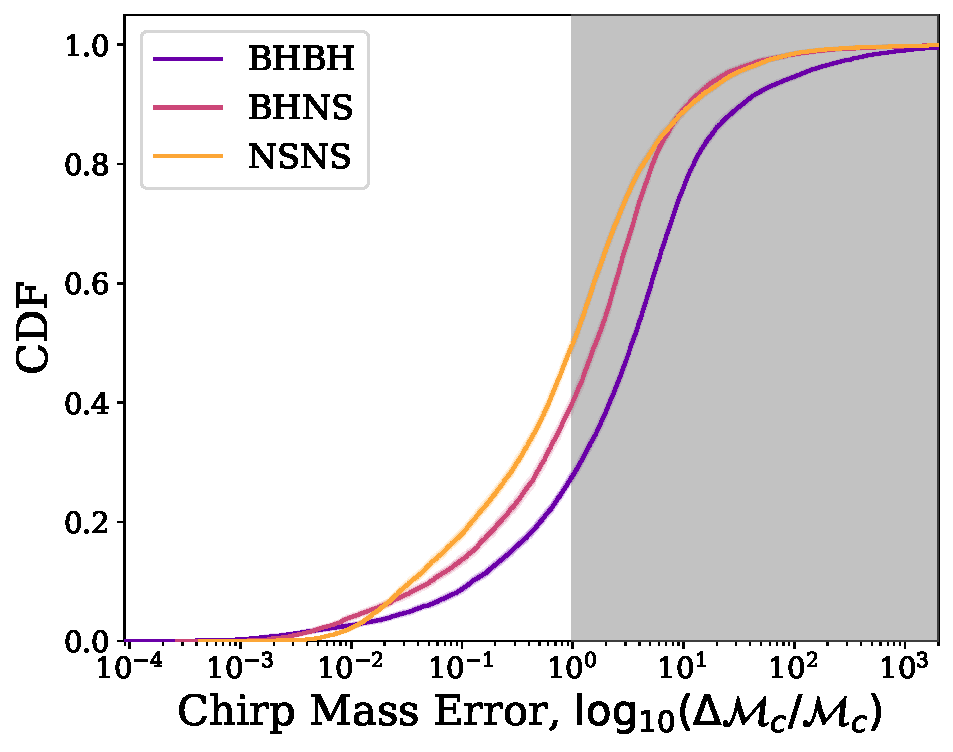
\includegraphics[width=\columnwidth]{chirp_mass_uncertainty_4yr.pdf}
    \caption{Cumulative distribution function for error on the chirp mass. Colours indicate DCO type and shading shows 1- and 2-$\sigma$ uncertainties (obtained via bootstrapping). Shaded region indicates region with unmeasureable chirp mass.}
    \label{fig:m_c_unc}
\end{figure}

\subsubsection{Sky localisation}
We quantify the sky localisation of a source by calculating its angular resolution. Since we find that all potential sources are stationary on the timescale of the LISA mission, following \citet{Mandel+2018}, we can use the timing accuracy of LISA and the effective detector baseline to calculate the angular resolution, $\sigma_{\theta}$, as
\begin{equation}
    \sigma_{\theta} = 16.6^\circ \left(\frac{7}{\rho}\right) \left(\frac{5 \times 10^{-4} \unit{Hz}}{f_{\rm dom}}\right) \left( \frac{2 \unit{AU}}{L} \right),
\end{equation}
where $L$ is the effective detector baseline, which for LISA is 2 AU since it will orbit the Sun.

We plot the angular resolution in Fig.~\ref{fig:ang_res}. The area of a patch on the sky that can be attributed to a source is given by $A = \pi \sigma_\theta^2$. From this plot, we see that the majority of sources can be resolved to an angular resolution of 10 degrees. The size of a pencil beam for a 15m diameter SKA dish observing at 1.4 GHz is roughly 0.67 square degrees, corresponding to an angular resolution of $\sigma_\theta = \sqrt{(0.67 / \pi)} = 0.46^\circ$ (which, for intuition, is approximately the angular size of the moon). Applying this to the plot shows that about 10-20\% of DCOs can be covered by a single pointing of SKA. However, since these LISA sources are essentially stationary in frequency space, observations need not be limited to a single pointing. We will discuss the prospects of matching LISA detections to radio pulsars with SKA further in Sec.~\ref{sec:pulsar_matching}.

\begin{figure}[ht]
    \centering
    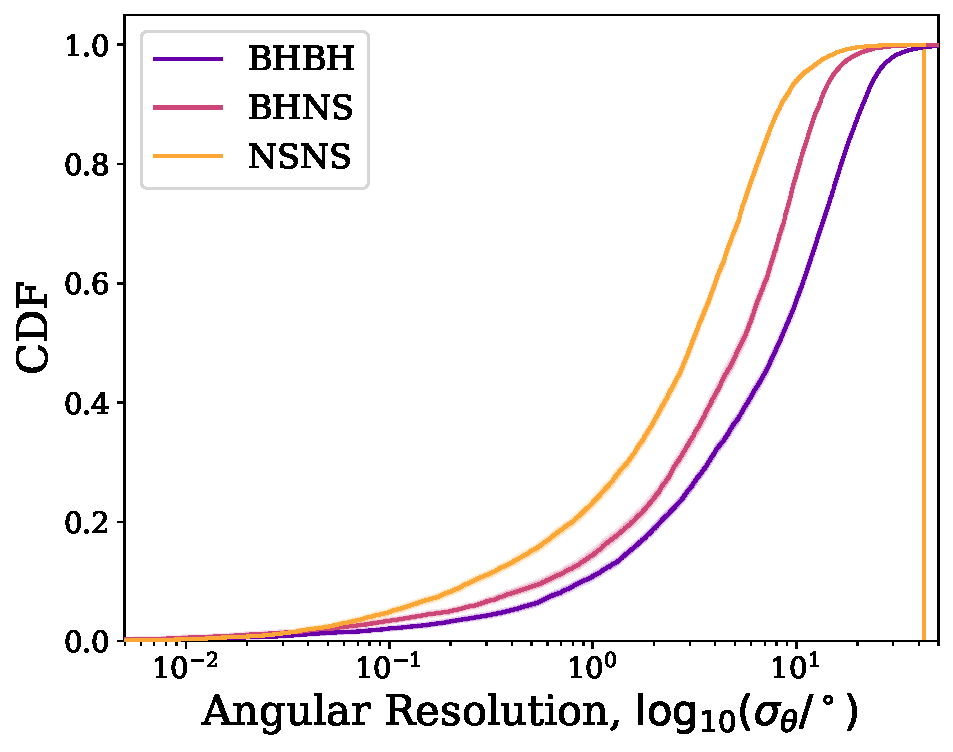
\includegraphics[width=\columnwidth]{angular_resolution_4yr.pdf}
    \caption{As Fig.~\ref{fig:m_c_unc}, but for the angular resolution.}
    \label{fig:ang_res}
\end{figure}


\section{Discussion} \label{sec:discussion}
In this section we discuss the prospects of (and methods for) identifying LISA sources (Sec.~\ref{sec:identify_sources}), the possibility of matching LISA signals to SKA detections (Sec.~\ref{sec:pulsar_matching}) and the main caveats for this study (Sec.~\ref{sec:caveats}).

\subsection{Identification of GW sources}\label{sec:identify_sources}
It is important to note that, though we present predictions for the detection rates of specific DCO types, the nature of the source may not be immediately apparent from the gravitational wave signal. The population of Galactic WDWDs detectable with LISA will be several orders of magnitude larger than the population of more massive DCOs that we focus on in this paper \citep[e.g.][]{Korol+2017}. It is therefore imperative that we consider how to distinguish NS and BH binaries from this much more numerous population of sources. In addition to distinguishing them from WDWDs, we must consider how to discriminate between BHBHs, BHNSs and NSNSs themselves.

\subsubsection{Distinguishing from WDWD population}\label{sec:WDWD_distinguish}
The simplest way to check whether a source is a WDWD is to check its chirp mass. The mass of a non-rotating white dwarf cannot be larger than the Chandrasekhar limit of $1.4 \unit{M_\odot}$ \citep{Chandrasekhar+1931, Hamada+1961}, so we can take the maximum chirp mass of a WDWD to be $\sim 1.2 \unit{M_{\odot}}$. Therefore, any DCO with a chirp mass that satisfies $\mathcal{M}_c > 1.2 \unit{M_{\odot}} + \Delta \mathcal{M}_c$ must not be a WDWD (where $\Delta \mathcal{M}_c$ is calculated using Eq.~\ref{eq:chirp_mass_uncertainty}). We find that for the detectable population of a 4(10)-year LISA mission, \BHBHAboveMaxWDWDFourPerc{}(\BHBHAboveMaxWDWDTenPerc{})\% of BHBHs, \BHNSAboveMaxWDWDFourPerc{}(\BHNSAboveMaxWDWDTenPerc{})\% of BHNSs and \NSNSAboveMaxWDWDFourPerc{}(\NSNSAboveMaxWDWDTenPerc{})\% of NSNSs satisfy this condition. This method is not particularly effective for NSNSs since their average chirp mass, $1.17 \unit{M_\odot}$, is below the Chandrasekhar limit.

Another discriminator between WDWDs and other DCOs is eccentricity. WDWDs formed in the disc are thought to be formed through isolated binary formation and have little to no eccentricity \citep[e.g.][]{Nelemans+2001}. Therefore, if any system is detected with anything other than one detectable harmonic, this suggests that the system is unlikely to be a WDWD. We find that for a 4(10)-year LISA mission, \BHBHMultipleHarmonicsFourPerc{}(\BHBHMultipleHarmonicsTenPerc{})\% of BHBHs, \BHNSMultipleHarmonicsFourPerc{}(\BHNSMultipleHarmonicsTenPerc{})\% of BHNSs and \NSNSMultipleHarmonicsFourPerc(\NSNSMultipleHarmonicsTenPerc{})\% of NSNSs are detected with multiple harmonics. Both the absolute percentage and the relative improvement with an extended LISA mission is lower for the BHNSs with respect to other DCOs as we find that these BHNSs are less eccentric on average (see Fig.~\ref{fig:fiducial_pdf_distributions} and discussion in Sec.~\ref{sec:fiducial_distributions}).

However, we should also consider that eccentric WDWDs could be formed through dynamical formation in Milky Way globular clusters \citep[e.g.][]{Willems+2007, Kremer+2018}. This means that we cannot assume that eccentric binaries are not WDWDs unless they are detected in the Galactic plane. We can use the sky localisation, scale height of the disc and distance to the source to estimate what fraction of eccentric sources can be localised to the Galactic plane. This condition can be written as $\sigma_\theta < \arcsin(z_{\rm plane} / D_L)$ or $D_L < z_{\rm plane}$, where we set the height of the Galactic plane, $z_{\rm plane}=0.95 \unit{kpc}$, to the scale height of the high-$\alpha$ disc. We apply this condition to find that the fraction of sources that are eccentric \textit{and} localised within the disc for a 4(10)-year LISA mission are \BHBHEccInDiscFourPerc{}(\BHBHEccInDiscTenPerc{})\% for BHBHs, \BHNSEccInDiscFourPerc{}(\BHNSEccInDiscTenPerc{})\% for BHNSs and \NSNSEccInDiscFourPerc{}(\NSNSEccInDiscTenPerc{})\% for NSNSs. Note that although the fractions are the same for the 10-year mission, the \textit{absolute} number of detections is still greater.

Overall, combining these methods we find that for a 4(10)-year mission, LISA will detect at least \BHBHNotWDWDFour{}(\BHBHNotWDWDTen{}) BHBHs, \BHNSNotWDWDFour{}(\BHNSNotWDWDTen{}) BHNSs and \NSNSNotWDWDFour{}(\NSNSNotWDWDTen{}) NSNSs that are distinguishable from the WDWD population.

We highlight here that, though the overall number of LISA detections in an extended mission only increases by a factor of $\sqrt{T_{\rm obs}}$, the number of \textit{distinguishable} detections increases by a greater factor since each of the more numerous sources are better measured. This further underlines the benefits of extending the LISA mission to 10 years.

\subsubsection{Discriminating between BHBHs, BHNSs and NSNSs}

The problem of discriminating between the BHBH, BHNS and NSNS populations can be more difficult than distinguishing them from WDWDs. For NSNSs, we can follow a similar method to the WDWDs (see Sec.~\ref{sec:WDWD_distinguish}) by applying our knowledge of the maximum mass of a neutron star. Following our fiducial assumption, we can take the maximum mass of a neutron star as $2.5 \unit{M_{\odot}}$ and thus the maximum chirp mass that a system can attain without one of the components being a black hole is $\mathcal{M}_{c} = 2.2 \unit{M_\odot}$. For a 4(10)-year LISA mission, the fraction of systems that are above or below this limit (and thus \textit{must} respectively contain or not contain a BH component) by more than $\Delta \mathcal{M}_c$ is \BHBHEitherBHOrNSFourPerc{}(\BHBHEitherBHOrNSTenPerc{})\% for BHBHs, \BHNSEitherBHOrNSFourPerc{}(\BHNSEitherBHOrNSTenPerc{})\% for BHNSs and \NSNSEitherBHOrNSFourPerc{}(\NSNSEitherBHOrNSTenPerc{})\% of NSNSs, which in terms of absolute detections is \BHBHEitherBHOrNSFour{}(\BHBHEitherBHOrNSTen{}) for BHBHs, \BHNSEitherBHOrNSFour{}(\BHNSEitherBHOrNSTen{}) for BHNSs and \NSNSEitherBHOrNSFour{}(\NSNSEitherBHOrNSTen{}) for NSNSs.

For separating the BHBH and BHNS population one could do so probabilistically given the properties that are measured, particularly the orbital frequency, mass ratio and eccentricity, since these distributions are fairly different for the two DCO types (see Fig.~\ref{fig:fiducial_pdf_distributions}). This method would pose a challenge however as it would likely only indicate which type was more likely rather than discriminate between them with strong evidence.

Another possible solution would be the existence of electromagnetic counterparts to the gravitational wave signal. In Section~\ref{sec:pulsar_matching} we consider the possibility of detecting a pulsar within a BHNS or NSNS system. This could be used to identify the type of the source.

\subsection{Matching LISA detections to pulsars with SKA}\label{sec:pulsar_matching}
Since the vast majority of the LISA detectable population of DCOs will not merge for many years, the main type of electromagnetic counterpart for this population is pulsars. Therefore, for this section we focus only on BHNSs and NSNSs since no BHBH system will contain a pulsar. The joint detection of a binary pulsar with LISA and SKA would not only help to constrain the parameters of the binary, but also enable investigation of other compact object physics. A pulsar(PSR)+BH can provide stringent tests of theories of gravity, in particular the ``No-hair theorem'' \citep{Keane+2015}. Alternatively, an ultrarelativstic PSR+NS system could be used to measure the neutron star equation of state up to an order of magnitude more accurately than other proposed observational constraints \citep{Kyutoku+2019, Thrane+2020}.

We estimate on average, given the number of detectable pulsars and SKA sky area, each pulsar in SKA occupies a region with an angular resolution of $\sigma_{\theta} < 1.3^\circ$ or $0.7^\circ$ for SKA-1 and SKA-2 respectively (see Appendix~\ref{app:ska_area}). Therefore, any DCOs containing NSs localised by LISA with an angular resolution lower than these values can be unambiguously matched to the radio signal in SKA. By considering Fig.~\ref{fig:ang_res}, approximately $11$ and $6$ (for SKA-1 and SKA-2) DCOs will satisfy this constraint.

If there is more than one pulsar in the region given by the LISA sky localisation, one can compare the measured parameters of the system in LISA and SKA. Both SKA and LISA will measure the orbital frequency to high precision, as well as the time derivative of the frequency and chirp mass to a lesser precision, of each of these systems. Therefore, one could perform a targeted search with SKA that checks the sky location given by LISA and only looking for binary pulsars with orbital frequencies within the uncertainties. If there was \textit{still} more than one possible pulsar one could also check against the chirp mass. In this way, we expect it will be possible to get a joint detection between SKA and LISA even when the sky area implied by the LISA detection contains more than one pulsar.

In order to assess the efficacy of this method, we would need to know the probability that two random binary pulsars would have orbital frequencies and chirp masses close enough that one could not tell which pulsar matches the LISA detection. This would require simulating the SKA population of pulsars with a code such as PSRPOPPy \citep{Bates+2014} to find the frequency and chirp mass distribution, which is beyond the scope of this paper. However, the uncertainty on the orbital frequency of a binary on the detection threshold (${\rm SNR} = 7$) for a 4-year LISA mission is $2.5 \times 10^{-9} \unit{Hz}$ and $1.0 \times 10^{-9} \unit{Hz}$ for a 10-year mission (calculated using Eq.~\ref{eq:f_orb_unc}). Therefore, we expect that SKA could likely isolate the correct binary pulsar to match to a LISA detection even when several are present in the sky localisation region.

\subsection{Caveats}\label{sec:caveats}

\textit{Population synthesis limitations:} As with any study involving a rapid population synthesis code, our results rely on uncertain stellar and binary physics and the use of approximate fitting formulae. COMPAS uses fitting formulae and approximate prescriptions based on (sometimes limited) grids of detailed models to describe the evolution of binary stars. Much of the underlying physics is uncertain, such as the common-envelope evolution and mass transfer physics. We attempt to understand the importance of some these assumptions by varying over many different physics assumptions.

\textit{Large progenitor masses:} Many of the black holes that are formed in our sample come from progenitors with large initial masses. The primary stars in systems that form  BHNSs and BHBHs have very primary progenitor masses that peak around 50\Msun and 80\Msun, but they extend well beyond that. The evolution of such massive progenitor stars is very poorly understood and observational constraints are very scarce in this mass range and practically non existent for the later rapid evolutionary phases.  This is reason for very substantial uncertainties in our final predictions which are unfortunately still hard to quantify at present. Additionally, the COMPAS code relies on fitting formula tat need to be extrapolated to create tracks are extrapolations at these higher masses. 

\textit{Underlying helium star models:} One source of weakness is that the \citet{Hurley+2000} fitting formulae for the evolution of helium stars are based on a grid of models from $0.3 \unit{M_{\odot}}$ to $10 \unit{M_{\odot}}$, for a single metallicity ($Z= 0.02$) and thus the formulae have no metallicity dependence and are extrapolated for higher masses. A more comprehensive set of models in this regime could lead to large changes in the evolution of naked helium stars, a common progenitor of DCOs, and thus affect the detection rate of DCOs.

\textit{Limited metallicity range:} The stellar evolution fitting formulae that COMPAS uses is that they are limited to a metallicity range of $10^{-4} \le Z \le 0.03$ \citep{Hurley+2000} and should not be extrapolated too far outside this range. However, in our simulated Milky Way (based on the metallicity relation in \citealt{Frankel+2018}), the metallicity distribution can extend as far as $10^{-5} \le Z \le 0.06$, with a significant fraction of star formation occurring past $Z = 0.03$. 

For metallicities below our range we assume they evolve similar to our lowest metallicity models. DCO formation at metallicities above $Z = 0.03$ is 
less efficient at high metallicity and so higher metallicities are unlikely to contribute significantly. Therefore, we place any sampled metallicity above the maximum of $Z = 0.03$ uniformly randomly in one of the top 5 highest bins that range across $0.01416 < Z < 0.03$ (since using a single metallicity for many binaries leads to unphysical artifacts).

\textit{Normalisation choices}: The choice of the binary fraction has a strong effect on our results. For the normalisation of the detection rate we conservatively choose to set the binary fraction of all stars to 50\%. The binary fraction is uncertain and not well constrained, though we know it is higher for more massive stars \citep[e.g.][]{Sana+2012}. Increasing it to 70\% and 100\% would increase our expected detection rates for every physics variation by 30\% and 67\% respectively. Moreover, we assume that the mass ratio of secondary stars is uniformly distributed and this could also have strong effect on our results. We highlight this uncertainty in the normalisation to point out that the exact magnitude of the rates in each case could change drastically as our understanding shifts. However, changes to this normalisation would affect every variation equally and so the trends across variations are more robust.

\textit{Systemic kicks:} We do not include the effect of systemic kicks on the final location of the sources. This would require integrating the orbital evolution of the millions of binaries in our sample and thus was not computationally reasonable to include. We investigated the effect of kicks for a small grid of binaries and found that, though they would result in a more spread out distribution (with a smaller concentration in the Galactic centre) and larger heights above the plane, the overall distribution of positions would be relatively unchanged and very few sources have strong enough kicks to reach escape velocity for the Milky Way.

\textit{Eccentricity measurement uncertainty:} The method that we use to determine the eccentricity uncertainty is pessimistic as it requires each harmonic to be individually detectable \citep[e.g.][]{Lau+2020}. In reality this may not be necessary depending on the efficacy of matched-filter analysis of LISA data. For an eccentric source to have been detected within the LISA data, several harmonics would already have to have been matched as originating from the same source. This could be done by looking in the same region of the sky for signals with similar chirp masses and distances to the most detectable harmonic in order to find other harmonics that are below the regular detection threshold. This would allow one to refine the measurement of the eccentricity uncertainty significantly by comparing the many different harmonics. Therefore, the eccentricity uncertainty that we calculate in this study is a pessimistic estimate. Smaller eccentricity uncertainties would have two main effects on our results. Firstly, the chirp mass error would decrease slightly in the cases where it is dominated by the eccentricity uncertainty. However, it is mainly dominated by the frequency derivative uncertainty since most sources are essentially stationary in frequency. Secondly, it would improve our ability to distinguish between WDWDs and higher mass DCOs. Until we know more about how LISA will search for eccentric sources, we rely upon our pessimistic estimates.

%\textit{Other formation channels:} We also note that our findings are only the result of a single formation channel (isolated binary formation). We do not consider other channels such as dynamical formation or chemically homogeneous evolution, which could increase the detection rate and alter the parameter distributions. For instance, \citet{Kremer+2018} predict that around $21$ systems could be detected in Milky Way globular clusters with LISA, formed through dynamical formation and thus different channels can still contribute significantly to the detection rate.

\textit{Other formation channels, the Halo, globular clusters and young stellar clusters:} Our model for the Milky Way, though more extensive than many previous studies, does not consider the contributions from the Galactic halo, globular clusters or young massive and open stellar clusters. \citet{Lamberts+2018} found that the halo's contribution to the detection rate was minimal and, since the metallicity distribution of the halo is uncertain, we did not include it in our galaxy model. The impact of globular clusters would have required a more detailed look into dynamical formation that was beyond the scope of this paper but we again highlight the work of \citet{Kremer+2018} that investigated these rates. Similarly, we did not consider DCO formation in young massive and open stellar clusters but \citet{Banerjee+2020} finds that the LISA detection rates could be even higher than contributions from isolated binary formation.



\section{Comparison with previous studies}\label{sec:compare_studies}
\begin{figure*}[p]
    \centering
    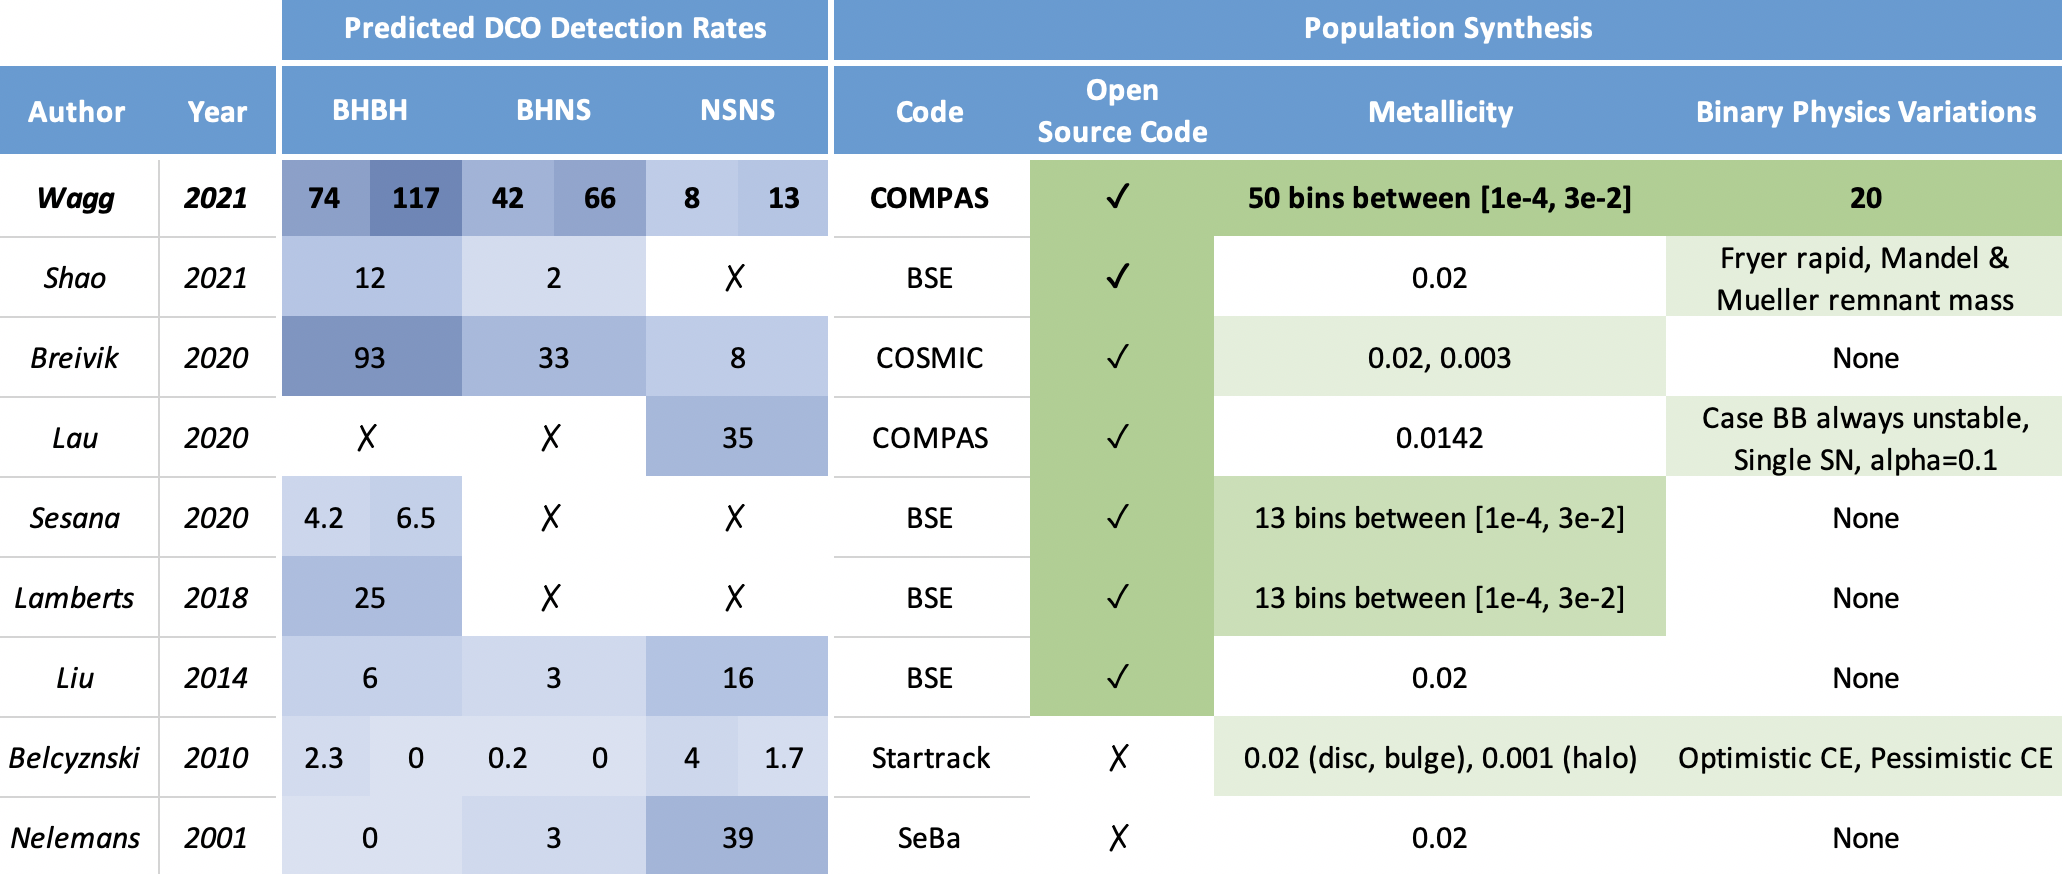
\includegraphics[width=\textwidth]{fig10_1_compare_dco.png}

    \vspace{0.5cm}

    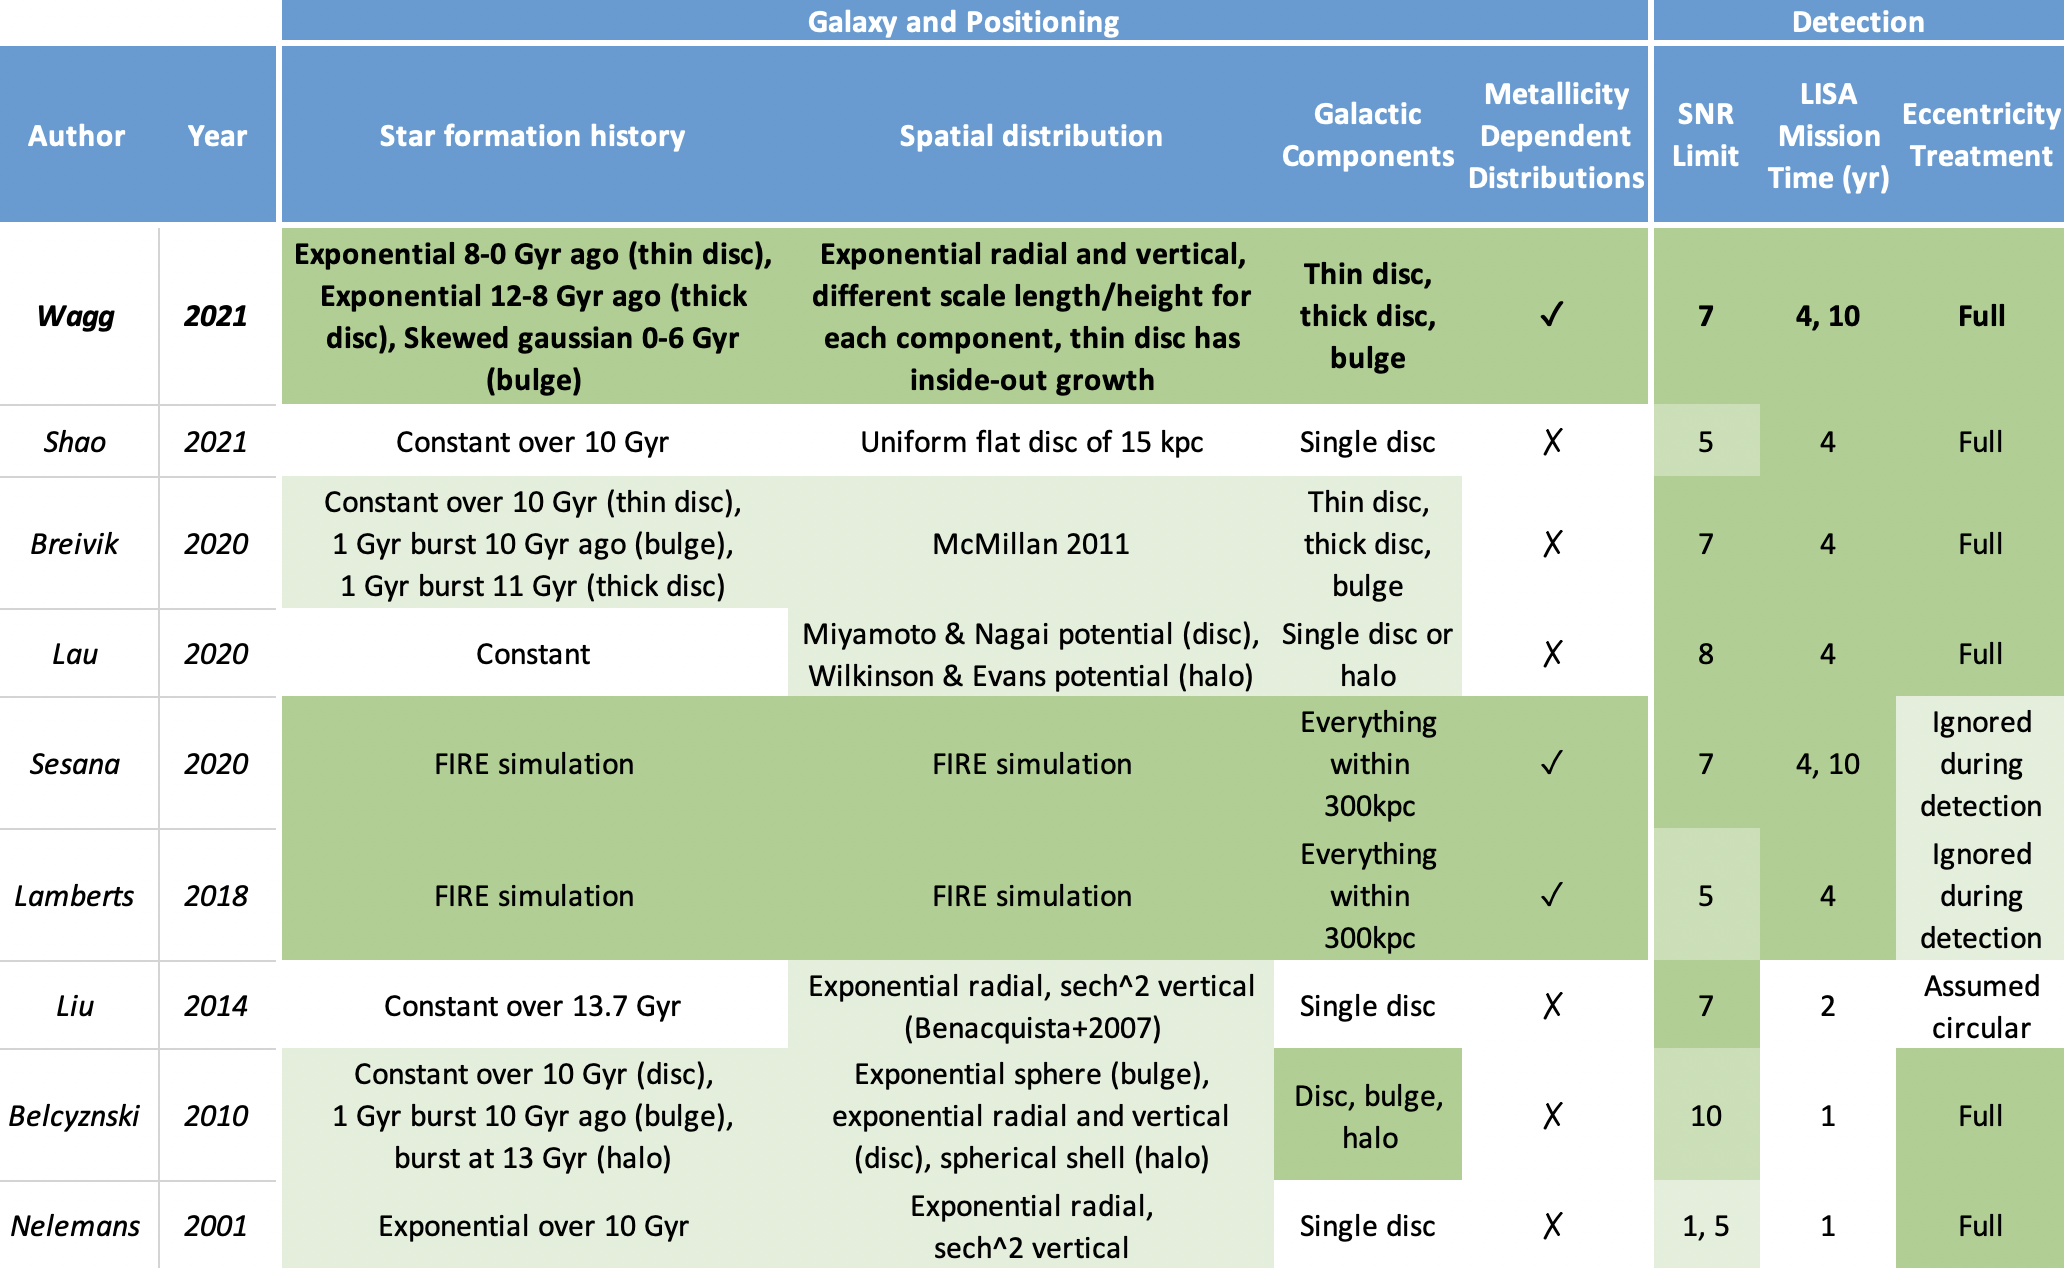
\includegraphics[width=\textwidth]{fig10_2_compare_dco.png}
    \caption{A table comparing previous studies of a similar nature to this work. The works listed in the table are \citet{Nelemans+2001}, \citet{Belczynski+2010}, \citet{Liu+2014}, \citet{Lamberts+2018}, \citet{Sesana+2020}, \citet{Lau+2020}, \citet{Breivik+2020} and \citet{Shao+2021}. \href{https://github.com/TomWagg/detecting-DCOs-in-LISA/blob/main/paper/figures/fig10_1_compare_dco.png}{\faFileImage} \href{https://github.com/TomWagg/detecting-DCOs-in-LISA/blob/main/paper/figures/fig10_w_compare_dco.png}{\faFileImage}.}
    \label{fig:previous_studies}
\end{figure*}

In Figure~\ref{fig:previous_studies}, we compare our results to similar previous studies that investigate the population of stellar-mass BHBHs, BHNSs and NSNSs that are detectable with LISA. Figure~\ref{fig:previous_studies} details the expected detection rates predicted by each paper as well as their assumptions regarding their Milky Way galaxy model, binary population synthesis simulation and LISA mission specifications. We only include papers that are similar to our work, such that they use population synthesis and simulate sources in the Galactic plane. Moreover, Figure~\ref{fig:previous_studies} does not include the numerous papers on the LISA WDWD population as we do not make predictions for these DCOs.
 
\paragraph{\citet{Nelemans+2001}} were the first to investigate the population of LISA detectable stellar-mass double compact objects. We find a significantly higher detection rate for BHBHs and BHNSs, as well as a slightly lower rate for NSNSs. We can understand this difference from changes both to the specifications of LISA (such as the mission length and SNR threshold for detection) and our understanding of massive star evolution since the publication of their paper, which both strongly affect the expected detections rates.

\paragraph{\citet{Belczynski+2010}} built upon the work of \citet{Nelemans+2001}, by using a different population synthesis code with two model variations and a multi-component model for the Milky Way. They find a much lower detection rate for BHNSs and NSNSs (and agreed on zero BHBHs) when compared to \citet{Nelemans+2001}. They state that this discrepancy from \citet{Nelemans+2001} comes from differences in their population synthesis and an overall lower formation rate rather than any changes to LISA detectability. The low total detection rate for all DCOs in this paper compared to our work is unsurprising given the relatively high SNR threshold of 10 and short mission length of 1 year. The reduced mission length means that the source signal has much less time to accumulate, whilst also fewer WDWDs can be resolved in this time, leading to a weaker signal and an increased Galactic confusion noise relative to our work.

\paragraph{\citet{Liu+2014}} performed a similar investigation using a different population synthesis code and find higher rates than earlier works. Their lower detection threshold and longer mission length compared to \citet{Belczynski+2010} likely explains the relatively increased rates. Yet their rates are still significantly below what we find. This could be for several reasons; they assume all binaries are circular both in their evolution and for detection. This means that systems may not have inspiralled as far before the LISA mission or may appear to have weaker gravitational waves when eccentricity is not accounted for. They also use a simplified model for the Milky Way with a single disc of one metallicity and constant star formation, whilst also using a mission length half what we assume. Each of these factors likely contributes to the lower overall detection rates.

\paragraph{\citet{Lamberts+2018}} presented a new approach to the problem by using the FIRE simulation \citep{Hopkins+2014} to distribute their sources rather than an analytical model of the Milky Way and were the first paper in this area to incorporate metallicity dependence into their Milky Way model. \citet{Sesana+2020} followed up on this paper using the same simulated BHBH population and presented updated results for the number of expected BHBH detections. They find significantly fewer BHBHs than our fiducial model despite using the same SNR threshold and LISA mission length.
%
The discrepancy between the results of \citet{Sesana+2020} and those presented in this work could be caused by different treatments of eccentricity. Unlike our work, \citet{Sesana+2020} assume that all binaries are circular for the purpose of detection in LISA, which could result in a lower number of detections by missing eccentric binaries that appear as weaker signals when assumed to be circular. This is especially relevant as we find that around $\BHBHNotCirc{}$ of LISA detectable BHBHs are not circular and around $\BHBHHighlyEccentric{}$ have significant eccentricity (see Section~\ref{sec:fiducial_distributions}). We also improve upon this work by using a larger number of metallicity bins compared to \citet{Sesana+2020}, since a low number of metallicity bins can produce artificial features in the mass distribution of DCOs and possibly affect the detection rate (see Appendix~\ref{app:mw_changes}). Finally, it could be that different implicit assumptions in their population synthesis code lead to differences in our results \citep{Toonen+2014}.

\paragraph{\citet{Lau+2020}} focussed on the number of Galactic NSNS binaries that could be detected by LISA. Their study uses the same population synthesis code, COMPAS, as this work, though an earlier version. Despite this, their study finds a much larger number of detections. They make several different physical assumptions in their population synthesis, using the \citet{Fryer+2012} \textit{rapid} remnant mass prescription, limiting the maximum neutron star mass to $2 \unit{M_{\odot}}$ and not implementing PISN. However, we note that none of these assumptions strongly affect the NSNS LISA detection rate (see bottom panel of Fig.~\ref{fig:detection_rates}, models \modRapid{}, \modNSLow{} and \modNoPISN{}) and so this is unlikely to entirely account for our differences. It is also important to highlight that COMPAS has received several improvements and bug fixes since \citet{Vigna-Gomez+2018} (which contains the simulations used by \citet{Lau+2020}) and these could possibly have affected the formation rate of NSNSs.
%
Yet it is most likely that the remaining difference between our results is due to way in which we simulate the Milky Way. \citet{Lau+2020} use a model for the Milky Way similar to that of \citet{Breivik+2020}, which we use to estimate the impact of the choice of MW model is in Appendix~\ref{app:mw_changes}. We find that this simpler model for the Milky Way could result in an overestimation of the NSNS detection rate by at least a factor of two and so this may explain the discrepancy between our results. \citet{Lau+2020} additionally only uses a single metallicity rather than the two used in \citet{Breivik+2020} and so the overestimation could be even stronger as their results will have no contribution from lower metallicity systems.

\paragraph{\citet{Breivik+2020}} introduced the population synthesis code COSMIC and presented detections for many different DCO types in LISA using this code. They find that LISA will detect 93 BHBHs, 33 BHNSs and 8 NSNSs in the Milky Way over a 4 year mission. \citet{Breivik+2020} make many different physical assumptions from us, the most notable being that they assume the optimistic CE scenario and that case BB mass transfer is always unstable, whilst also using a simpler model for the Milky Way (see Appendix~\ref{app:mw_changes}). Thus for better comparison we ran our simulation using model \modCaseBBOpt{} and the Milky Way model from \citet{Breivik+2020}. This results in 97, 101 and 43 detections for BHBHs, BHNSs and NSNSs respectively. Therefore, though we are in very good agreement for BHBHs, we predict much higher rates for BHNSs and NSNSs. These differences are likely due to using a different population synthesis code (COSMIC), which has different underlying physics assumptions from COMPAS. Given our strong agreement for BHBHs, it is possible that COSMIC and COMPAS handle NSs differently and so lead to different detection rates for DCOs containing NSs. However checking this would require a more in-depth study of the intrinsic formation rate of DCOs containing NSs in the two codes.

\paragraph{\citet{Shao+2021}} most recently investigated the detectability binaries containing BHs in LISA using BSE and a relatively simple model for the Milky Way (assuming a uniform flat disc, constant star formation and a single metallicity). They assume that kicks for NSs formed through ECSN are slightly higher than our work ($50 \unit{km}{s^{-1}}$ instead of $30 \unit{km}{s^{-1}}$). This may account for their particularly low BHNS rate (as the binaries would be more likely to disrupt), which is a factor of 20 lower than ours, but we expect their assumption of the optimistic CE scenario, reduced Wolf-Rayet winds and lower SNR detection threshold would offset this. As we show in Appendix~\ref{app:mw_changes}, their use of a simpler Milky Way model, especially with only a single metallicity, would lead to an underestimate of the BHBH and BHNS rates, which may explain the discrepancy in our results.

\section{Conclusion \& Summary} \label{sec:conclusion}
We provide predictions for the detection rate and population properties of LISA detectable BHBH, BHNS and NSNS.
To this end, we use the rapid population synthesis code COMPAS to simulate over two billion massive binaries, to explore the effect of varying underlying physics assumptions that represent the most common uncertainties in binary physics. We use an new empirically-informed analytical model to distribute the resulting BHBH, BHNS and NSNS populations in a Milky-Way like galaxy based on their birth metallicity, in order to estimate and investigate the LISA detectable population of BH and NS binaries.

Our main conclusions can be summarised as:
\begin{enumerate}
    \item \textbf{Detections:} We predict 30-300 detections in a 4-year LISA mission, across all our simulations for varying physics assumptions. Although the number of detections per type can vary by about 2 orders of magnitude, we find that the total detection rate is fairly robust, among the variations we have considered.
    
    Specifically, our fiducial model predicts a total of $124 \pm 11$ detections and out of these we find about $\BHBHFourYear{}\pm 9$ BHBHs, $\BHNSFourYear{}\pm 6$ BHNSs and $\NSNSFourYear{}\pm 3$ NSNSs. The errors quoted here are the $1$-$\sigma$ Poisson uncertainties resulting from the random initialisation of the Milky Way (see Table~\ref{tab:detection_rates}).
    
    \item \textbf{Benefits of extended LISA mission} Increasing the LISA mission length to 10 years results increases the number of detections to about 50-500 detections, a 60\% increase, because the number of detections scale approximately as $T_{\rm obs}^{0.5}$.
%    
    However, the real benefit is the improvement of the characterisation of the sources, since the relative error on the frequency derivative (which dominates the relative error in the chirp mass) scales as $T_{\rm obs}^{-2.5}$  for stationary sources (Eq.~\ref{eq:f_orb_dot_unc}).
    
    We find an increase of a factor 2.4 for the number of systems with chirp masses that can be measured better than 10\%. 
%    
    The number of systems with a sky localisation better than one degree increases by about 50\%.
%    
    The number of sources that can be unambiguously distinguished from WDWDs increases by almost a factor 2 (see Section~\ref{sec:WDWD_distinguish}).
    
    \item \textbf{Probing the black hole mass distribution and the lower mass gap:} We expect LISA to predominantly detect lower mass BHs (with 90\% of BHBH and BHNSs having BH masses lower than $11 \unit{M_\odot}$ in our fiducial simulations) in stark contrast to current ground-based detectors which are heavily biased towards high mass systems. This implies that LISA can potentially make important contributions to the debate about the existence of a lower mass gap (\citealt{Shao+2021} and see our Fig.~\ref{fig:lower_mass_gap_variation}).
    
    \item \textbf{Eccentricity distribution:} We find that for all DCO types a large fraction of detectable systems still have nonzero eccentricities ($e = 0.01$) when entering the LISA band, unlike what is expected for the more numerous WDWD LISA population. In particular, we find that this is the case for the vast majority of BHBHs and NSNSs and nearly half of BHNSs. Furthermore, over a fifth of detectable BHBHs have eccentricities large enough such that their primary gravitational wave emission occurs in a higher harmonic ($e > 0.3$).
    
    % We predict that for the observed population \BHBHNotCirc{}(\BHBHHighlyEccentric{}) of BHBHs, \BHNSNotCirc{}(\BHNSHighlyEccentric{}) of BHNSs and \NSNSNotCirc{}(\NSNSHighlyEccentric{})\% of NSNSs have eccentricity of $e > 0.01(0.3)$ at the start of the LISA mission.
    \item \sout{\textbf{Physics variations:} For BHBHs, we find that the detection rate is largely unaffected by changes in underlying physics assumptions, except for the optimistic CE scenario and increased Wolf-Rayet winds. Conversely, the BHNS detection rate varies widely with physics variation, ranging across three orders of magnitude. The NSNS detection rate shows some variation but only shows large changes under the assumption that case BB mass transfer is unstable and that core-collapse supernovae produce weaker kicks.} - We have now said most of this is point 1. We could additionally talk about \textit{which} assumptions are causing the largest variations.
    \item \textbf{Source identification:} For a 4(10)-year LISA mission we estimate that, of the detectable population, at least \BHBHNotWDWDFour{}(\BHBHNotWDWDTen{}) BHBHs, \BHNSNotWDWDFour{}(\BHNSNotWDWDTen{}) BHNSs and \NSNSNotWDWDFour{}(\NSNSNotWDWDTen{}) NSNSs will produce signals that are distinguishable from a signal produced by a WDWD. Additionally, we predict that we will be able to determine whether \BHBHEitherBHOrNSFour{}(\BHBHEitherBHOrNSTen{}) BHBHs, \BHNSEitherBHOrNSFour{}(\BHNSEitherBHOrNSTen{}) BHNSs and \NSNSEitherBHOrNSFour{}(\NSNSEitherBHOrNSTen{}) NSNSs are signals from a binary that contains a black hole.
    \item \textbf{Joint SKA-LISA detections:} We expect that \textit{if} every LISA detectable DCO contained a pulsar that is beaming towards Earth, SKA-1 would be able to detect at least 11 of these objects, whilst the increased number of detectable pulsars that could crowd the sky with SKA-2 sensitivity means that this total decreases to 6. This number is a pessimistic estimate and could be much higher if we consider that SKA and LISA could match their orbital frequency estimates to select the correct pulsar from a crowded field.
    \item \textbf{Importance of choice of MW model:} Many studies use Milky Way models that use fixed metallicity populations which are assigned irrespective of birth time or position, do not account for the inside-out growth of the thin disc and use constant star formation rates. The use of these simpler MW models may lead to an overestimation of the LISA NSNS detection rate and an underestimation of the BHNS detection rate. It may also introduce unphysical artifacts into DCO parameter distributions, particularly the mass distributions, which lead to inaccurate predictions.
\end{enumerate}


\software{COMPAS (version 02.12.00) \url{http://github.com/TeamCOMPAS/COMPAS}. \citep{Stevenson+2017, Vigna-Gomez+2018, Broekgaarden+2019}, \texttt{Python} available from \url{python.org}, matplotlib \citep{Hunter+2007},  \texttt{NumPy} \citep{vanderWalt+2011}, 
Astropy \citep[\url{http://www.astropy.org}][]{AstropyCollaboration+2013, AstropyCollaboration+2018}.}

\acknowledgments{We thank Mike Lau, Floris Kummer, Eva Laplace, Rob Farmer, Katie Sharpe, Mathieu Renzo, Katie Brevik, Alberto Sesana, Valeriya Korol, Will Farr and the members of the COMPAS collaboration for insightful discussions. This project was funded in part by the European Union’s Horizon 2020 research and innovation program from the European Research Council (ERC, Grant agreement No. 715063), and by the Netherlands Organization for Scientific Research (NWO) as part of the Vidi research program BinWaves with project number 639.042.728. We further acknowledge the Black Hole Initiative funded by a generous contribution of the John Templeton Foundation and the Gordon and Betty Moore Foundation.}

\clearpage

\bibliographystyle{aasjournal}
\bibliography{references}

\allowdisplaybreaks
\appendix
\section{Population Synthesis}\label{app:pop_synth}

In this section we summarise the main assumptions and settings from the population synthesis simulation from \citet{Broekgaarden+2021,Broekgaarden+2021b}.

\subsection{Initial conditions}

\citet{Broekgaarden+2021,Broekgaarden+2021b} simulate between 1 and 100 million massive binaries for each of 50 metallicities equally spaced in log space between $Z \in [0.0001, 0.022]$, where $Z$ is the mass fraction of heavy elements. They simulate more binaries for higher metallicities so that large enough sample of DCOs at each metallicity (since DCOs are formed at a lower rate at higher metallicities). These metallicities span the allowed metallicity range for the original fitting formulae on which COMPAS is based \citep{Hurley+2000}. This is repeated for \nMinusOneModels{} physics variations (see Section \ref{sec:variation_assumptions}) and so in total over two billion binaries were simulated.

Each binary is sampled from initial distributions for the primary and secondary masses as well as the separation. The primary mass, that is the mass of the initially more massive star, is restricted to $m_1 \in [5, 150] \unit{M_{\odot}}$, which spans the range of interest for NS and BH formation in binary systems, and drawn from the \citet{Kroupa+2001} initial mass function (IMF), $p(m_1) \propto m_1^{-2.3}$. The secondary mass, $m_2$, is drawn using the initial mass ratio of the binary, $q \equiv m_2 / m_1$, which \citet{Broekgaarden+2021,Broekgaarden+2021b} assume to be uniform on $[0, 1]$, therefore $p(q) = 1$ \citep[e.g.\ consistent with][]{Sana+2012}. They additionally restrict the secondary masses $m_2 \ge 0.1 \unit{M_{\odot}}$, which is approximately the minimum mass for a main sequence star. They assume that the initial separation follows a flat in the log distribution with $p(a_i) \propto 1 / a_i$ and $a_i \in [0.01, 1000] \unit{AU}$ \citep{Opik+1924, Abt+1983}. They assume that all binary orbits are circular at birth to reduce the dimensions of initial parameters. Since they focus on post-interaction binaries which will have circularised after mass transfer they argue this is an reasonable assumption (as many studies have in the past) and is likely not critical for predicting detection rates \citep{Hurley+2002, deMink+2015}.

\citet{Broekgaarden+2021,Broekgaarden+2021b} apply the adaptive importance sampling algorithm STROOPWAFEL \citep{Broekgaarden+2019} to improve the yield of their sample. This algorithm increases the prevalence of target DCOs (BHBHs, BHNSs and NSNSs in this case) in the sample and assigns each a weight, $w$, which represents the probability of drawing the DCO without STROOPWAFEL in effect.

\subsection{Physical assumptions in the fiducial model}\label{app:fiducial_physics}

\textit{Stellar Evolution:} To follow the evolution of massive stars, COMPAS relies on fitting formulae by \citet{Hurley+2000} to detailed single star models by \citet{Pols+1998}. COMPAS models the evolution of stars that lose or gain mass closely following the algorithms originally described in \citet{Tout+1996} and \citet{Hurley+2002}.

\textit{Wind mass loss:} \citet{Broekgaarden+2021,Broekgaarden+2021b} follow the wind prescription from \citet{Belczynski+2008}, which was based on results from Monte Carlo radiative transfer simulation of \citet{Vink+2000, Vink+2001}. They use the wind mass loss rates from \citet{Vink+2001} for stars above $12500 \unit{K}$ and the rates from \citet{Hurley+2000} for cooler stars. Additionally, they use a separate, higher wind mass loss rate for luminous blue variable (LBV) stars, following \citet{Belczynski+2008}, to mimic observed LBV eruptions for stars with luminosities and effective temperatures above the Humphreys-Davidson limit. They use the Wolf-Rayet-like mass loss rate from \citet{Hamann+1998} with an additional metallicity scaling from \citet{Vink+2005} for helium stars, and set $f_{\rm WR} = 1$. See \citet{COMPAS:2021methodsPaper}, Section 3 for the explicit equations.

\textit{Mass Transfer:} In determining the stability of mass transfer \citet{Broekgaarden+2021,Broekgaarden+2021b} use the $\zeta$-prescription, which compares the radial response of the star with the response of the Roche lobe radius to the mass transfer \citep[e.g.][]{Hjellming+1987}. The mass transfer efficiency, $\beta \equiv \Delta M_{\rm acc} / \Delta M_{\rm don}$, is the fraction of the mass transferred by the donor that is actually accreted by the accretor. They limit the maximum accretion rate for stars to $\Delta M_{\rm acc} / \Delta t \le 10 M_{\rm acc} / \tau_{\rm KH}$, where $\tau_{\rm KH}$ is the Kelvin-Helmholtz timescale of the star \citep{Paczynski+1972, Hurley+2002}. The maximum accretion rate for compact objects is limited to the Eddington accretion rate. If more mass than these rates is accreted then they assume that the excess is lost through isotropic re-emission in the vicinity of the accreting star \citep[e.g.][]{Massevitch+1975, Soberman+1997}. They assume that all mass transfer from a stripped post-helium-burning-star (case BB) onto a neutron star or black hole is unstable \citep{Tauris+2015}.

\textit{Common-Envelope:} A common-envelope phase follows dynamically unstable mass transfer and \citet{Broekgaarden+2021,Broekgaarden+2021b} parameterise this using the $\alpha$-$\lambda$ prescription from \citet{Webbink+1984} and \citet{deKool+1990}. They assume $\alpha = 1$, such that all of the gravitational binding energy is available for the ejection of the envelope. For $\lambda$ they use the fitting formulae from \citet{Xu+2010, Xu+2010a}. They assume that any Hertzsprung gap donor stars that initiate a common-envelope phase will not survive this phase due to a lack of a steep density gradient between the core and envelope \citep{Taam+2000, Ivanova+2004, Klencki+2021}. This follows the `pessimistic' common-envelope scenario \citep[c.f.][]{Belczynski+2007}. They remove any binaries where the secondary immediately fills its Roche lobe upon the conclusion of the common-envelope phase as they treat these as failed common-envelope ejections, likely leading to a stellar merger.

\textit{Supernovae:} \citet{Broekgaarden+2021,Broekgaarden+2021b} draw the remnant masses and natal kick magnitudes from different distributions depending on the type of supernova that occurs. For stars undergoing a general core-collapse supernova, they use the \textit{delayed} supernova remnant mass prescription from \citet{Fryer+2012}. The \textit{delayed} prescription does not reproduce a neutron star black hole mass gap and they use this as their default as it has been shown to provide a better fit for observed populations of DCOs \citep[e.g.][]{Vigna-Gomez+2018}. They draw the natal kick magnitudes from a Maxwellian velocity distribution with a one-dimensional root-mean-square velocity dispersion of $\sigma_{\rm rms}^{\rm 1D} = 265 \unit{km}{s^{-1}}$ \citep{Lyne+1994, Hobbs+2005}. They assume that stars with helium core masses between $1.6$--$2.25 \unit{M_{\odot}}$ \citep{Hurley+2002} experience electron-capture supernovae (ECSN) \citep{Nomoto+1984, Nomoto+1987, Ivanova+2008}. They set all remnant masses to $1.26 \unit{M_{\odot}}$ in this case as an approximation of the solution to Equation 8 of \citet{Timmes+1996}. For these supernovae, they set $\sigma_{\rm rms}^{\rm 1D} = 30 \unit{km}{s^{-1}}$ \citep[e.g.][]{Pfahl+2002, Podsiadlowski+2004}. They assume that stars that undergo case BB mass transfer \citep{Dewi+2002} experience extreme stripping which leads to an ultra-stripped supernova \citep{Tauris+2013, Tauris+2015}. For these supernovae they calculate the remnant mass using the \citet{Fryer+2012} prescription and use $\sigma_{\rm rms}^{\rm 1D} = 30 \unit{km}{s^{-1}}$ (as with ECSN). Stars with final helium core masses between $35$-$135 \unit{M_{\odot}}$ are presumed to undergo a pair-instability, or pulsational pair-instability supernova \citep[e.g.][]{Woosley+2007, Farmer+2019}. They follow the prescription from \citet{Marchant+2019} as implemented in \citep{Stevenson+2019} for these supernovae. They assume that kicks are isotropic in the frame of the collapsing star. They adopt a maximum neutron star mass of $2.5 \unit{M_{\odot}}$ \citep[e.g.][]{Kalogera+1996, Fryer+2015, Margalit+2017} for the fiducial model and change the \citet{Fryer+2012} prescription accordingly.

\subsection{Model variations} \label{sec:variation_assumptions}
In addition to their fiducial model for the formation of DCOs, \citet{Broekgaarden+2021,Broekgaarden+2021b} explore \nMinusOneModels{} other models in which they change various aspects of the mass transfer, common-envelope, supernova and wind mass loss physics assumptions in order to assess the effect of their uncertainties on the overall double compact object detection rates and distributions. Each of the models varies a single physics assumption (fiducial assumptions are outlined in Section~\ref{app:fiducial_physics}) and these models are outlined in Table~\ref{tab:physics_variations}.

Their fiducial model is labelled model \modFid{}. Models \modRangeMT{} focus on changes to the mass transfer physics assumptions. They explore the effect of fixing the mass transfer efficiency $\beta$ to a constant value, rather than allowing it to vary based on the maximum accretion rate. In models \modBetaLow{}, \modBetaMed{}, \modBetaHigh{}, in which they set the value of $\beta$ to $0.25$, $0.5$ and $0.75$ respectively.

Models \modRangeCE{} focus on altering the common-envelope physics. In model \modCaseBB{} we modify model E from \citet{Broekgaarden+2021,Broekgaarden+2021b} to investigate the consequence of assuming that case BB mass transfer is always unstable, whilst allowing Helium HG donors to survive CE events. They change the common-envelope efficiency parameter to $\alpha_{\rm CE} = 0.1, 0.5, 2.0, 10.0$ in models \modAlphaLowest{}, \modAlphaLow{}, \modAlphaHigh{} and \modAlphaHighest{} respectively. In model \modOpt{}, they relax their restriction that Hertzsprung gap donor stars cannot survive common-envelope events, thereby following the `optimistic' common-envelope scenario. They combine this with model \modCaseBB{} in model \modCaseBBOpt{}.

In models \modRangeSN{} they consider changes related to their assumptions about supernova physics. Model \modRapid{} uses the alternate \textit{rapid} remnant mass prescription from \citet{Fryer+2012} instead of the \textit{delayed} prescription. They change the maximum neutron star mass in models \modNSLow{} and \modNSHigh{} to $2$ and $3 \unit{M_{\odot}}$ respectively to account for the range of predicted maximum neutron star masses. Model \modNoPISN{} removes the implementation of pair-instability and pulsational pair-instability supernovae. In models \modSigLow{} and \modSigLower{} they decrease the root-mean-square velocity dispersion for core-collapse supernovae to explore the effect of lower kicks. Model \modNoBH{} removes the natal kick for all black holes.

Finally, in models \modRangeML{} \citet{Broekgaarden+2021,Broekgaarden+2021b} investigate the effect of changing their assumption about wind mass loss rates, specifically for Wolf-Rayet winds. They vary $f_{\rm WR}$ to $0.1$ and $5.0$ in models \modWRLow{} and \modWRHigh{} respectively. These values approximately span the current range of possible Wolf-Rayet wind efficiencies suggested from observations \citep[e.g.][]{Vink+2017, Hamann+2019, Shenar+2019, Miller-Jones+2021, vanSon+2021}.

\begin{table}[htb]
    \centering
    \begin{tabular}{cl}
        \hline \hline
        Model & Physics Variation \\
        \hline \hline
        \modFid & Fiducial (see Section~\ref{app:fiducial_physics}) \\
        \hline
        \modBetaLow & Fixed mass transfer efficiency of $\beta=0.25$ \\ 
        \modBetaMed & Fixed mass transfer efficiency of $\beta=0.5$  \\ 
        \modBetaHigh & Fixed mass transfer efficiency of $\beta=0.75$ \\
        \hline
        \modCaseBB & Case BB mass transfer always unstable \\
        \modCaseBBOpt & Case BB always unstable + Optimistic CE \\
        \modAlphaLowest & CE efficiency parameter $\alpha = 0.1$ \\
        \modAlphaLow & CE efficiency parameter $\alpha = 0.5$ \\
        \modAlphaHigh & CE efficiency parameter $\alpha = 2$   \\
        \modAlphaHighest & CE efficiency parameter $\alpha = 10$   \\
        \modOpt & HG donor stars initiating a CE survive CE \\
        \hline
        \modRapid & Fryer rapid SN remnant mass prescription \\
        \modNSLow & Maximum NS mass is fixed to $2\unit{M_{\rm \odot}}$ \\
        \modNSHigh & Maximum NS mass is fixed to $3\unit{M_{\rm \odot}}$ \\
        \modNoPISN & PISN and pulsational-PISN not implemented \\
        \modSigLow & $\sigma_{\rm{rms}}^{\rm{1D}}=100 \unit{km}{s^{-1}}$ for core-collapse supernova \\  
        \modSigLower & $\sigma_{\rm{rms}}^{\rm{1D}}=30  \unit{km}{s^{-1}}$ for core-collapse supernova \\ 
        \modNoBH & Black holes receive no natal kick \\
        \hline
        \modWRLow & Wolf-Rayet wind factor $f_{\rm WR} = 0.1$ \\
        \modWRHigh & Wolf-Rayet wind factor $f_{\rm WR} = 5.0$ \\
        \hline \hline
    \end{tabular}%
    \caption{A description of the \nModels{} binary population synthesis models used in this study. \modFid{} is the fiducial model, \modRangeMT{} change mass transfer physics, \modRangeCE{} change common-envelope physics , \modRangeSN{} change supernova physics and \modRangeML{} change wind mass loss \citep[c.f.][Table 2]{Broekgaarden+2021}.}
    \label{tab:physics_variations}
\end{table}


\section{Detection Rate Normalisation}\label{app:rate_normalisation}
In this section we explain the normalisation process that we refer to in Section~\ref{sec:gw_detection}. From each simulated instance of the Milky Way we extract the fraction of targets that are detectable, where we define a target as one of BHBH, BHNS or NSNS that merges in a Hubble time. To convert the detectable fraction to a detection rate for the Milky Way, we write that the \textit{number} of detectable targets in the Milky Way is
\begin{equation}\label{eq:norm_frame}
    N_{\rm detect} = f_{\rm detect} \cdot N_{\rm target, MW},
\end{equation}
where $f_{\rm detect}$ is the fraction of targets in the instance that were detectable and $N_{\rm target, MW}$ is the total number of targets that have been formed in the Milky Way's history. We can further break this total down into
\begin{equation}
    N_{\rm target, MW} = \avg{ \mathcal{R}_{\rm target} } \cdot M_{\rm SF, MW},
\end{equation}
where $\avg{ \mathcal{R}_{\rm target} }$ is the average number of targets formed per star forming mass and $M_{\rm SF, MW}$ is the star forming mass of the Milky Way, meaning the total mass of every star ever formed in the Milky Way.

\subsection{Average target formation rate}
Double compact object formation is metallicity dependent, so we find the average rate as the integral over metallicity, which is given by
\begin{equation}\label{eq:norm_avg_target_formation}
    \avg{ \mathcal{R}_{\rm target} } = \int_{Z_{\rm min}}^{Z_{\rm max}} p_{Z} \mathcal{R}_{\rm target, Z} \dd{Z},
\end{equation}
where $Z_{\rm min}, Z_{\rm max}$ are the minimum and maximum sampled metallicities, $p_Z$ is the probability of forming a star at the metallicity $Z$ (which can be found using the distribution in \citealp{Frankel+2018}) and $\mathcal{R}_{\rm target, Z}$ is the number of targets formed per star forming mass,
\begin{equation}
    \mathcal{R}_{\rm target, Z} =  \frac{N_{\rm target, Z}}{ M_{\rm SF, Z} }.
\end{equation}
In practice, this integral is instead approximated as a sum over the metallicity bins that we use in our simulation. The number of targets in our sample at a metallicity $Z$, $N_{\rm target, Z}$, can be written simply as the sum of the targets' weights:
\begin{equation}
    N_{\rm target, Z} = \sum_{i=1}^{N_{\rm binaries, Z}} w_i \theta_{\rm target, i},
\end{equation}
where $w_i$ is the binary's adaptive importance sampling weight assigned, $N_{\rm binaries, Z}$ is the number of binaries at metallicity $Z$ in our sample and $\theta_{\rm target, i}$ is only $1$ when the binary is a target and otherwise $0$.

The total star forming mass at a metallicity $Z$, $M_{\rm SF, Z}$, can be written as
\begin{equation}
    M_{\rm SF, Z} = \frac{\avg{m}_{\rm COMPAS, Z}}{f_{\rm trunc}} N_{\rm binaries, Z},
\end{equation}
where $\avg{m}_{\rm COMPAS}$ is the average star forming mass of a binary in a simulation using our cutoffs (discussed in Section~\ref{sec:COMPAS_explained}) and $f_{\rm trunc}$ is the fraction of the total stellar mass from which our COMPAS simulations sample, given our truncated mass and separation ranges (see Section~\ref{sec:COMPAS_explained}). These truncations mean that only $f_{\rm trunc} \approx 0.17$ of the stellar mass in the galaxy is sampled from.

\subsection{Total star forming mass in the Milky Way}
It is important to distinguish between the \textit{total} mass of every star formed over the entire history of the Milky Way and the \textit{current} stellar mass in the Milky Way. Many stars born in the Milky Way are no longer living and have lost much of their mass to stellar winds and supernovae, thus the current stellar mass in the Milky Way is an underestimate of the total star forming mass.

\citet{Licquia+2015} find that the total stellar mass today in the Milky Way is $6.08 \pm 1.14 \times 10^{10} \unit{M_{\odot}}$. This total includes all stars and stellar remnants (white dwarfs, neutrons stars and black holes) but \textit{excludes} brown dwarfs. We can write that the total mass of every star every formed in the Milky Way is
\begin{equation}\label{eq:m_SF_MW}
    M_{\rm SF, MW} = (6.08 \pm 1.14) \times 10^{10} \unit{M_{\rm \odot}} \cdot \frac{\avg{m}_{\rm SF, total}}{\avg{m}_{\rm SF, today}},
\end{equation}
where $\avg{m}_{\rm SF, total}$ is the average mass of a star over the history of the Milky Way and is defined as
\begin{equation}
    \avg{m}_{\rm SF, total} = \int_{0}^{t_{\rm MW}} p_{\rm birth}(\tau) \int_{0.01}^{200} \zeta(m)\ m \dd{m} \dd{\tau},
\end{equation}
where $t_{\rm MW}$ is the age of the Milky Way, $\zeta(m)$ is the \citet{Kroupa+2001} IMF function and $p_{\rm birth}(\tau)$ is the probability of a star being formed at a lookback time $\tau$ (Eq.~\ref{eq:thin_disc_tau}). $\avg{m}_{\rm SF, today}$ is the average mass of all stars and stellar remnants (excluding brown dwarfs) present in the Milky Way today is defined as follows (note that we integrate from $0.08$ not $0.01$ since observations of today's Milky Way mass exclude brown dwarfs)
\begin{equation}
    \avg{m}_{\rm SF, today} = \int_{0}^{t_{\rm MW}} p_{\rm birth}(\tau) \int_{0.08}^{200} \zeta(m)\ m_{\rm today} \dd{m} \dd{\tau},
\end{equation}
where $m_{\rm today}(m, Z, \tau)$ is the current mass of a star that was formed $\tau$ years ago at a metallicity $Z$. We calculate $m_{\rm today}(m, Z, \tau)$ by interpolating the final masses given by COMPAS for a grid of single stars over different masses and metallicities using the \citet{Fryer+2012} delayed prescription and default wind mass loss settings. For $Z$, we use the average star forming metallicity in the Milky Way at a lookback time $\tau$ using our galaxy model. Evaluating Equation~\ref{eq:m_SF_MW}, we find that the total mass of every star that has ever formed in the Milky Way is
\begin{align}
    M_{\rm SF, MW} &= (6.1 \pm 1.1) \times 10^{10} \unit{M_{\odot}} \cdot \frac{0.378 \unit{M_{\odot}}}{0.221 \unit{M_{\odot}}}, \nonumber \\
    &= (10.4 \pm 1.1) \times 10^{10} \unit{M_{\odot}},
\end{align}
an increase of approximately 70\% from the value still in stars today!

\subsection{Normalisation summary}
Finally, we can substitute Equations~\ref{eq:norm_avg_target_formation} and \ref{eq:m_SF_MW} into \ref{eq:norm_frame} and write that the overall normalisation of the detection rate is calculated as
\begin{align}
    N_{\rm detect} &= f_{\rm detect} \cdot 10.4 \times 10^{10} \unit{M_{\odot}} \nonumber \\
    &\times \sum_{Z=Z_{\rm min}}^{Z_{\rm max}} p_{Z} \qty(\sum_{i=1}^{N_{\rm binaries, Z}} w_i \theta_{\rm target, i}) \nonumber \\
    &\times \qty(\frac{\avg{m}_{\rm COMPAS, Z}}{f_{\rm trunc}} \sum_{i=1}^{N_{\rm binaries, Z}} w_i)^{-1}.
\end{align}

\section{Calculation of the uncertainties in the chirp mass for detectable sources}\label{app:chirp_mass_uncertainty}

How accurately the chirp mass of a detected binary can be determined depends on the signal to noise ratio, duration of the mission, its orbital frequency and the time derivative of the orbital frequency. 

Here we describe how we estimate the uncertainty of the chirp mass. First, consider the chirp mass, which can be expressed as
\begin{equation}
    \mathcal{M}_c = \frac{c^3}{G} \left( \frac{5 \pi}{48 n} \frac{\dot{f}_{n}}{F(e)} \right)^{3/5} \frac{1}{(2 \pi f_{\rm orb})^{11/5}},
\end{equation}
where ${f}_{n}$ is the frequency of the n-th harmonic,  $f_{\rm orb}$ is the orbital frequency, $\mathcal{M}_{c}$ is the chirp mass (defined in Eq.~\ref{eq:chirp_mass}), $e$ is the eccentricity and
\begin{equation}\label{eq:peters_f}
    F(e) = \frac{1 + \frac{73}{24} e^2 + \frac{37}{96} e^4}{(1 - e^2)^{7/2}},
\end{equation}
is the enhancement factor of gravitational wave emission for an eccentric binary over an otherwise identical circular binary \citep[][Eq.~17]{Peters+1963}. 
%
In practice, we will use the dominating harmonic, with $n=n_{\rm dom}$ and $f_n = n_{\rm dom} f_{\rm orb} = f_{\rm dom}$. The dominating harmonic for circular binaries is $n_{\rm dom} = 2$ and so the dominating frequency is twice the orbital frequency. 

Therefore the chirp mass uncertainty can be estimated as
\begin{equation}\label{eq:chirp_mass_uncertainty}
    \frac{\Delta \mathcal{M}_c}{\mathcal{M}_c} = \frac{11}{5} \frac{\Delta f_{\rm orb}}{f_{\rm orb}} + \frac{3}{5} \frac{\Delta \dot{f}_{\rm dom}}{\dot{f}_{\rm dom}} + \frac{3}{5} \frac{\Delta F(e)}{F(e)},
\end{equation}
%where $f_{\rm dom}$ is the harmonic frequency with the strongest SNR ($f_{\rm dom} = n_{\rm dom} f_{\rm orb}$ and $n_{\rm dom} = 2$ for circular binaries) as this will provide the best measurement.

We estimate the frequency uncertainties using \citet{Takahashi+2002}, such that
\begin{align}\label{eq:f_orb_unc}
    \frac{\Delta f_{\rm orb}}{f_{\rm orb}} &= 4 \sqrt{3} \cdot \frac{1}{\rho} \frac{1}{T_{\rm obs}} \frac{1}{f_{\rm orb}}, \\
    \frac{\Delta \dot{f}_{\rm dom}}{\dot{f}_{\rm dom}} &= 6 \sqrt{5} \cdot \frac{1}{\rho} \left(\frac{1}{T_{\rm obs}} \right)^2 \frac{1}{\dot{f}_{\rm dom}},\label{eq:f_orb_dot_unc}
\end{align}
where $\rho$ is the signal-to-noise ratio and $T_{\rm obs}$ is the LISA mission length. We estimate the eccentricity uncertainty, $\Delta e$, following the methods of \citet{Lau+2020} and \citet{Korol+2021}, which use the relative SNRs of different harmonics to work out the eccentricity. We propagate this uncertainty such that
\begin{equation}
    \frac{\Delta F(e)}{F(e)} = \Delta e \cdot \frac{(1256 + 1608 e^2 + 111 e^4) e}{96 + 196 e^2 - 255 e^4 - 37 e^6}.
\end{equation}

We use Eq.~\ref{eq:chirp_mass_uncertainty} to calculate the chirp mass uncertainty for each DCO type in our sample and plot it in Fig.~\ref{fig:m_c_unc}.


\section{Assessing the impact of Milky Way model choices}\label{app:mw_changes}
The model that we use for the Milky Way adds several layers of complexity, accounting for the inside-out growth of the thin disc, using empirically informed star formation histories that are a function of time and assigning metallicities based on the position and age of binaries. In this section, we repeat our main analysis but instead apply a simpler model for the Milky Way in order to assess the effect of these added features. For this purpose, we use model for the Milky Way used in \citet{Breivik+2020} as this is representative of the models used in most previous works.

Their model can be summarised as follows: the Milky Way is assumed to comprise of three components, a thin disc, a thick disc and a bulge. The spatial distributions and relative masses for these components are given in \citet{McMillan+2011}. \citet{Breivik+2020} assume constant star formation over 10 Gyr for the thin disc, a 1 Gyr burst of star formation 11 Gyr ago for the thick disc and a 1 Gyr burst of star formation 10 Gyr ago for the bulge. A major difference is that only two metallicities are used and they are assigned to binaries independent of age or position. Binaries formed in the thin disc and bulge are assumed to have a metallicity of $Z = 0.02$ and those formed in the thick disc are assumed to have $Z = 0.003$.

We show the spatial metallicity distribution for this model in Fig.~\ref{fig:simple_mw} in the same form as Fig.~\ref{fig:galaxy_schematic} for ease of comparison between our models. The two main differences we can see between Fig.~\ref{fig:galaxy_schematic} and \ref{fig:simple_mw} are that the \citet{Breivik+2020} model is more centrally concentrated and only has two fixed metallicity populations.

\begin{figure}[htb]
    \centering
    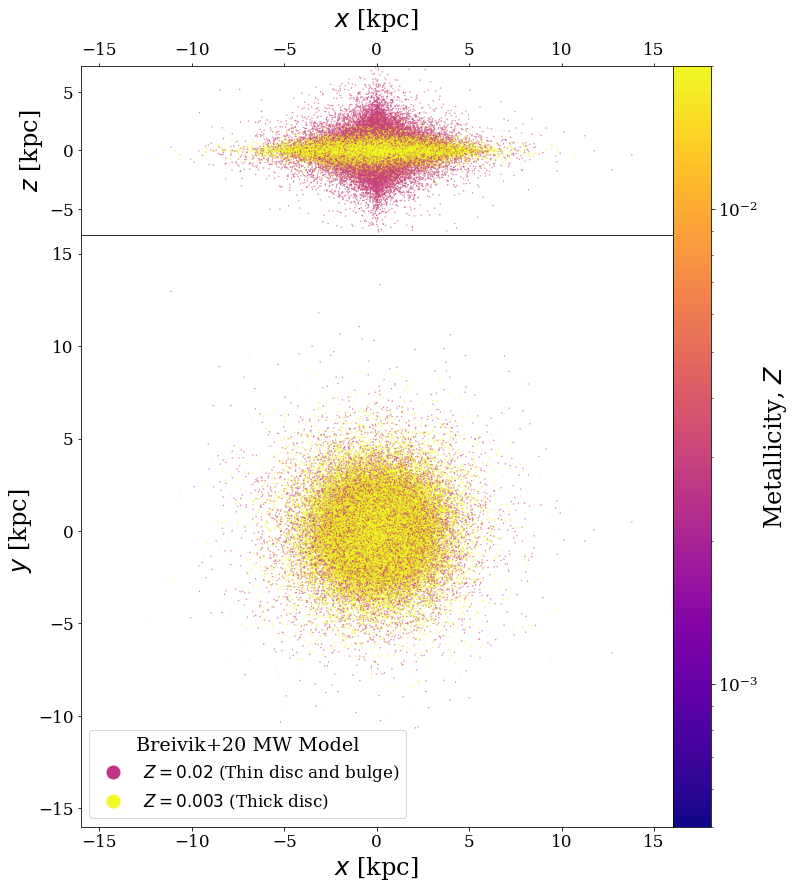
\includegraphics[width=\columnwidth]{figD1_random_simple_galaxy.png}
    \caption{As Fig.~\ref{fig:galaxy_schematic} (right panel), but for the Milky Way model used in \citet{Breivik+2020}.  \href{https://github.com/TomWagg/detecting-DCOs-in-LISA/blob/main/paper/figures/figD1_random_simple_galaxy.png}{\faFileImage} \href{https://github.com/TomWagg/detecting-DCOs-in-LISA/blob/main/paper/figure_notebooks/galaxy_creation_station.ipynb}{\faBook}.}
    \label{fig:simple_mw}
\end{figure}

When applying this simpler Milky Way model in combination with our fiducial binary physics assumptions (model \modFid{}), we find that the expected number of detections for BHBHs, BHNSs and NSNSs for a 4-year LISA mission is $52$, $25$ and $17$ respectively. Thus the BHBH detection has decreased slightly compared to our main findings, whilst for BHNSs and NSNSs the rate has approximately halved and doubled respectively.

Moreover, the distribution of parameters within the population, particularly the mass distributions, are notably disparate. By using only two fixed metallicity populations, unphysical artifacts are introduced into distribution of DCO masses \citep[e.g.][]{Dominik+2015, Neijssel+2019, Kummer_thesis}. For example, in Fig.~\ref{fig:bh_mass_simple_mw}, we show the black hole mass distribution \edit1{for BHNSs} produced by the simulation using the simple Milky Way model. Despite the fact that these KDEs use the same bandwidth as Fig.~\ref{fig:fiducial_pdf_distributions}, the distributions show many more sharp transitions, which is a result of pileups occurring at specific masses for specific metallicities. Moreover, the lack of lower metallicities systems means that higher mass systems are not formed and so we see the distributions do not include a high mass tail such as in our fiducial results.

The unphysical artifacts present in the mass distributions can have far-reaching effects since the masses of DCOs affect most other parameters. The inspiral time and SNR are directly dependent on the mass, whilst the uncertainty estimates depend on the SNR. This means that the artifacts can affect the predictions for most distributions of LISA detectable populations.

Overall, we find that previous studies that use Milky Way models analogous to this simpler model may significantly underestimate the LISA BHNS rate whilst overestimating the NSNS detection rate. They may also miss higher mass systems (particular for BHNSs) and contain unphysical artifacts in their parameter distributions.

\begin{figure}[htb]
    \centering
    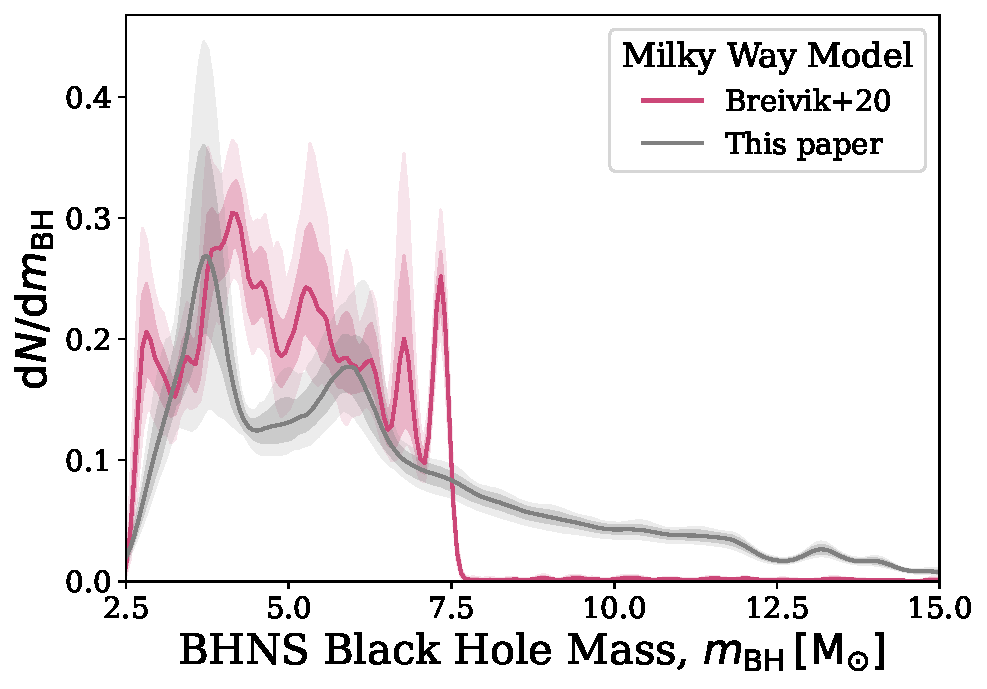
\includegraphics[width=\columnwidth]{figD2_mBH_simple_mw_variation.pdf}
    \caption{As Fig.~\ref{fig:fiducial_pdf_distributions}b, but for the Milky Way model used in \citet{Breivik+2020}. Dotted lines show the distribution from Fig.~\ref{fig:fiducial_pdf_distributions}b for comparison. \href{https://github.com/TomWagg/detecting-DCOs-in-LISA/blob/main/paper/figures/figD2_mBH_simple_mw_variation.pdf}{\faFileImage} \href{https://github.com/TomWagg/detecting-DCOs-in-LISA/blob/main/paper/figure_notebooks/fiducial.ipynb}{\faBook}.}
    \label{fig:bh_mass_simple_mw}
\end{figure}

\section{Estimating the number of pulsars for a given sky area in SKA}\label{app:ska_area}

In this section, we perform some back-of-the-envelope calculations in order to estimate the number of pulsars that SKA will observe within a given sky area.

First, we consider how many pulsars SKA is likely to detect. \citet{Keane+2015} uses PSRPOPPy \citep{Bates+2014} to simulate the Milky Way pulsar population. They find that for SKA-1, approximately $10000$ pulsars will be discovered. The second phase of SKA, which should be in operation by the time of the LISA mission, would yield a total of $35000$-$41000$ pulsars \citep{Keane+2015}. We use the average, $38000$, in further estimates below. Moreover, we are only interested in pulsars that are part of a binary system. We estimate this pulsar binary fraction as the fraction of known pulsars that are in binaries using the ATNF Pulsar Catalogue\footnote{\url{https://www.atnf.csiro.au/research/pulsar/psrcat}} \citep{Manchester+2005}. $290$ of the $2872$ currently known pulsars are in binary systems and thus we estimate the binary fraction of pulsars as $10\%$. Therefore, we expect that SKA-1 and SKA-2 will detect approximately $1000$ and $3800$ binary pulsars respectively.

Next, we can find the total number of pulsars SKA will detect in a patch on the sky. The total sky area that the SKA covers is approximately $5700 \unit{deg^2}$, which is calculated by integrating over the sky for all Galactic longitudes and Galactic latitudes limited to $\abs{b} < 10^\circ$ and $\delta < 45^\circ$, which are the limits on SKA-mid \citep{Keane+2015}. If we assume that the pulsars are found uniformly across the sky, this means that roughly $0.2$ and $0.7$ binary pulsars are expected per square degree for SKA-1 and SKA-2 respectively. Note that the assumption of a uniform distribution is not realistic as pulsars will tend to be far more concentrated in the Galactic centre but we use it to provide a slightly optimistic estimate.

Overall, we therefore expect a single pulsar per $5.7 \unit{deg^2}$ and $1.5 \unit{deg^2}$ for SKA-1 and SKA-2 respectively, which correspond to angular resolutions of $\sigma_\theta = 1.3^\circ$ and $\sigma_\theta = 0.7^\circ$.

\clearpage
\onecolumngrid

\section{Supplementary material}

\begin{table*}[htb]
    \centering
    \caption{The number of detectable binaries in a 4- and 10-year LISA mission for the \nModels{} different model variations and each DCO type. Each model variation is discussed in App.~\ref{sec:variation_assumptions} and the trends in detection rates are discussed in Sec.~\ref{sec:detection_rate_analysis}. The `All' column contains the total expected detections when summed over the three types. The final two rows show the minimum and maximum rates across all model variations. We embolden the corresponding rate for convenience of seeing which variation results in the minimum/maximum. Each value shows the mean and the 1-$\sigma$ Poisson uncertainty. \href{https://github.com/TomWagg/detecting-DCOs-in-LISA/blob/main/paper/figure_notebooks/detections.ipynb}{\faBook}.}
    \begin{tabular}{cl|cccc|cccc}
        \hline
        \multirow{2}{*}{Model} & \multirow{2}{*}{Description} & \multicolumn{4}{c|}{LISA detections (4 year)} & \multicolumn{4}{c}{LISA detections (10 year)} \\ \cline{3-10}
        & & {All} & {BHBH} & {BHNS} & {NSNS} & {All} & {BHBH} & {BHNS} & {NSNS} \\
        \hline
        A & Fiducial & \confinv{124}{11}{11} & \confinv{74}{9}{8} & \confinv{42}{6}{7} & \confinv{8}{3}{3} & \confinv{202}{15}{14} & \confinv{117}{10}{11} & \confinv{71}{8}{8} & \confinv{13}{4}{4}\\
        B & Fixed mass transfer efficiency of $\beta=0.25$ & \confinv{94}{10}{10} & \confinv{69}{9}{8} & \confinv{22}{4}{5} & \confinv{3}{2}{2} & \confinv{149}{12}{12} & \confinv{108}{11}{10} & \confinv{37}{6}{6} & \confinv{5}{2}{2}\\
        C & Fixed mass transfer efficiency of $\beta=0.5$ & \confinv{59}{8}{8} & \confinv{47}{7}{7} & \confinv{8}{3}{3} & \confinv{4}{2}{2} & \confinv{96}{10}{9} & \confinv{76}{9}{8} & \confinv{14}{4}{3} & \confinv{7}{3}{2}\\
        D & Fixed mass transfer efficiency of $\beta=0.75$ & \confinv{67}{8}{8} & \confinv{47}{7}{7} & \confinv{7}{2}{3} & \confinv{13}{4}{3} & \confinv{104}{10}{11} & \confinv{71}{8}{8} & \confinv{12}{3}{4} & \confinv{21}{4}{5}\\
        E$^\prime$ & Case BB mass transfer is always unstable & \confinv{90}{10}{9} & \confinv{66}{8}{8} & \confinv{21}{5}{5} & \boldconfinv{3}{2}{1} & \confinv{133}{11}{12} & \confinv{101}{10}{10} & \confinv{29}{5}{5} & \boldconfinv{4}{2}{2}\\
        F & Case BB Unstable + Optimistic CE & \boldconfinv{368}{19}{19} & \boldconfinv{154}{13}{12} & \boldconfinv{198}{14}{14} & \confinv{17}{4}{4} & \boldconfinv{553}{24}{23} & \boldconfinv{238}{15}{16} & \boldconfinv{289}{17}{17} & \confinv{25}{5}{5}\\
        G & CE efficiency $\alpha = 0.1$ & \confinv{40}{6}{6} & \confinv{28}{5}{5} & \boldconfinv{2}{1}{2} & \confinv{10}{3}{3} & \confinv{64}{8}{8} & \confinv{44}{7}{6} & \boldconfinv{3}{1}{2} & \confinv{17}{4}{4}\\
        H & CE efficiency $\alpha = 0.5$ & \confinv{86}{10}{9} & \confinv{58}{7}{8} & \confinv{22}{5}{4} & \confinv{6}{3}{2} & \confinv{136}{12}{11} & \confinv{91}{9}{10} & \confinv{35}{6}{6} & \confinv{10}{3}{3}\\
        I & CE efficiency $\alpha = 2.0$ & \confinv{133}{12}{11} & \confinv{67}{8}{9} & \confinv{38}{6}{6} & \confinv{28}{6}{5} & \confinv{218}{15}{14} & \confinv{109}{10}{11} & \confinv{62}{7}{8} & \confinv{46}{7}{7}\\
        J & CE efficiency $\alpha = 10.0$ & \confinv{78}{9}{9} & \confinv{27}{6}{5} & \confinv{16}{4}{4} & \boldconfinv{35}{6}{6} & \confinv{126}{11}{11} & \confinv{42}{6}{7} & \confinv{27}{6}{5} & \boldconfinv{57}{7}{8}\\
        K & HG donor stars initiating a CE survive CE & \confinv{218}{15}{14} & \confinv{151}{12}{12} & \confinv{57}{8}{7} & \confinv{10}{3}{3} & \confinv{340}{18}{19} & \confinv{229}{15}{15} & \confinv{96}{10}{10} & \confinv{16}{4}{4}\\
        L & Fryer rapid SN remnant mass prescription & \confinv{127}{11}{11} & \confinv{50}{7}{7} & \confinv{70}{8}{8} & \confinv{7}{3}{2} & \confinv{204}{14}{15} & \confinv{76}{8}{9} & \confinv{117}{11}{11} & \confinv{11}{3}{3}\\
        M & Maximum NS mass = 2.0 ${\rm M_{\odot}}$ & \confinv{133}{11}{12} & \confinv{96}{10}{10} & \confinv{30}{5}{5} & \confinv{7}{2}{3} & \confinv{214}{14}{15} & \confinv{153}{12}{13} & \confinv{50}{7}{7} & \confinv{12}{4}{3}\\
        N & Maximum NS mass = 3.0 ${\rm M_{\odot}}$ & \confinv{118}{11}{11} & \confinv{58}{8}{8} & \confinv{52}{7}{7} & \confinv{8}{3}{3} & \confinv{189}{13}{14} & \confinv{91}{9}{10} & \confinv{85}{10}{9} & \confinv{14}{4}{3}\\
        O & No PISN and pulsational-PISN & \confinv{126}{11}{12} & \confinv{75}{9}{9} & \confinv{43}{6}{7} & \confinv{8}{3}{3} & \confinv{205}{14}{14} & \confinv{120}{11}{11} & \confinv{72}{8}{9} & \confinv{13}{4}{3}\\
        P & $\sigma_{\rm RMS}^{\rm 1D} = 100 \ {\rm km\ s^{-1}}$ for CCSN & \confinv{184}{14}{14} & \confinv{82}{9}{9} & \confinv{86}{9}{10} & \confinv{15}{4}{4} & \confinv{300}{17}{17} & \confinv{130}{12}{11} & \confinv{145}{12}{12} & \confinv{26}{6}{5}\\
        Q & $\sigma_{\rm RMS}^{\rm 1D} = 30 \ {\rm km\ s^{-1}}$ for CCSN & \confinv{268}{16}{16} & \confinv{92}{10}{9} & \confinv{143}{12}{12} & \confinv{34}{6}{6} & \confinv{426}{20}{21} & \confinv{142}{11}{12} & \confinv{229}{16}{15} & \confinv{55}{7}{8}\\
        R & Black holes receive not natal kick & \confinv{205}{14}{15} & \confinv{89}{9}{10} & \confinv{109}{11}{10} & \confinv{7}{2}{3} & \confinv{332}{18}{18} & \confinv{140}{12}{12} & \confinv{180}{13}{13} & \confinv{12}{4}{3}\\
        S & Wolf-Rayet wind factor $f_{\rm WR} = 0.1$ & \confinv{118}{11}{11} & \confinv{75}{8}{9} & \confinv{34}{6}{6} & \confinv{9}{3}{3} & \confinv{182}{14}{13} & \confinv{112}{11}{11} & \confinv{56}{8}{7} & \confinv{14}{4}{4}\\
        T & Wolf-Rayet wind factor $f_{\rm WR} = 5.0$ & \boldconfinv{30}{6}{5} & \boldconfinv{6}{3}{2} & \confinv{15}{3}{4} & \confinv{8}{2}{3} & \boldconfinv{49}{7}{7} & \boldconfinv{9}{3}{3} & \confinv{26}{5}{5} & \confinv{13}{3}{4}\\
        \hline 
        - & Minimum rate & \confinv{30}{6}{5} & \confinv{6}{3}{2} & \confinv{2}{1}{2} & \confinv{3}{2}{1} & \confinv{49}{7}{7} & \confinv{9}{3}{3} & \confinv{3}{1}{2} & \confinv{4}{2}{2} \\
        - & Maximum rate & \confinv{368}{19}{19} & \confinv{154}{13}{12} & \confinv{198}{14}{14} & \confinv{35}{6}{6} & \confinv{553}{24}{23} & \confinv{238}{15}{16} & \confinv{289}{17}{17} & \confinv{57}{7}{8} \\
        \hline
    \end{tabular}
    \label{tab:detection_rates}
\end{table*}

\begin{figure}[p]
    \centering
    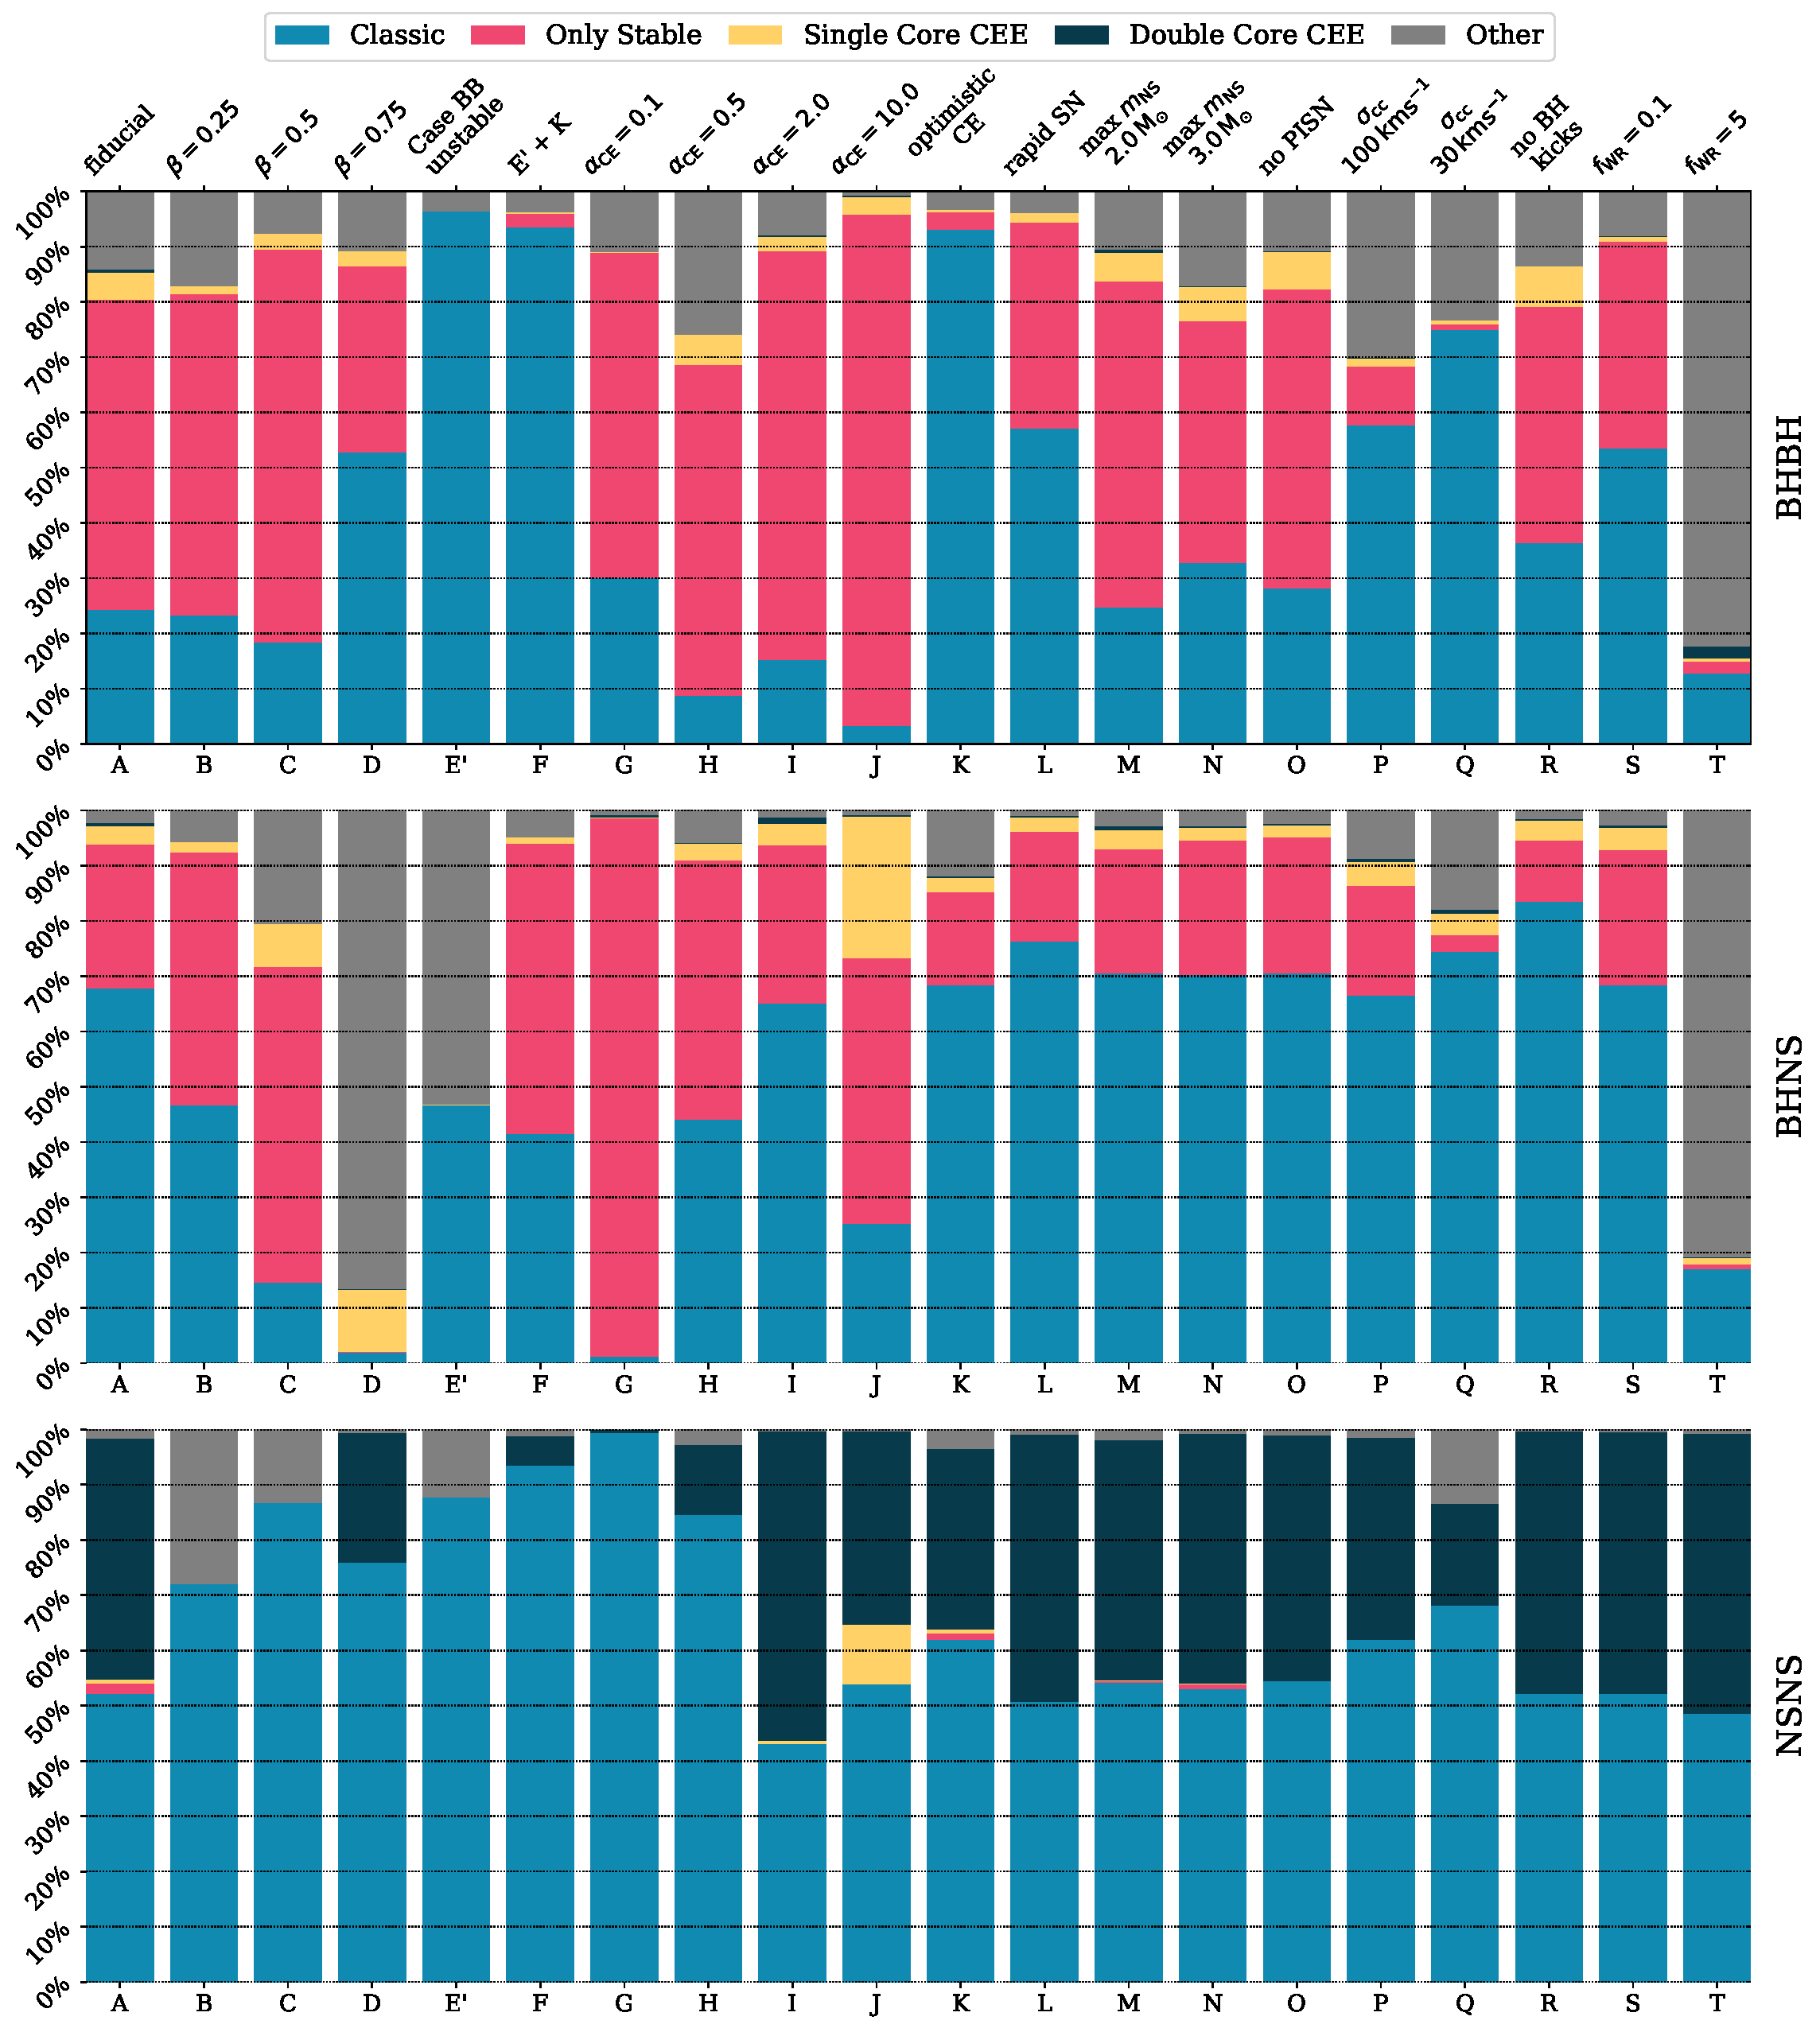
\includegraphics[height=0.85\textheight]{figF1_formation_channels.pdf}
    \caption{Fraction of each DCO type that is formed through different formation channels for all physics variations. Channels are described in detail in \citet{Broekgaarden+2021}. The classic, single core CEE and double core CEE channels all require at least one common-envelope event whilst only ``only stable'' consists of only stable mass transfer and ``other'' contains the remaining binaries which are mainly formed from case A ``classic'' binaries as well as ``lucky'' supernova kicks that shrink the binary. \href{https://github.com/TomWagg/detecting-DCOs-in-LISA/blob/main/paper/figures/figF1_formation_channels.pdf}{\faFileImage} \href{https://github.com/TomWagg/detecting-DCOs-in-LISA/blob/main/paper/figure_notebooks/formation_channels.ipynb}{\faBook}.}
    \label{fig:formation_channels}
\end{figure}

\begin{figure*}[p]
    \centering
    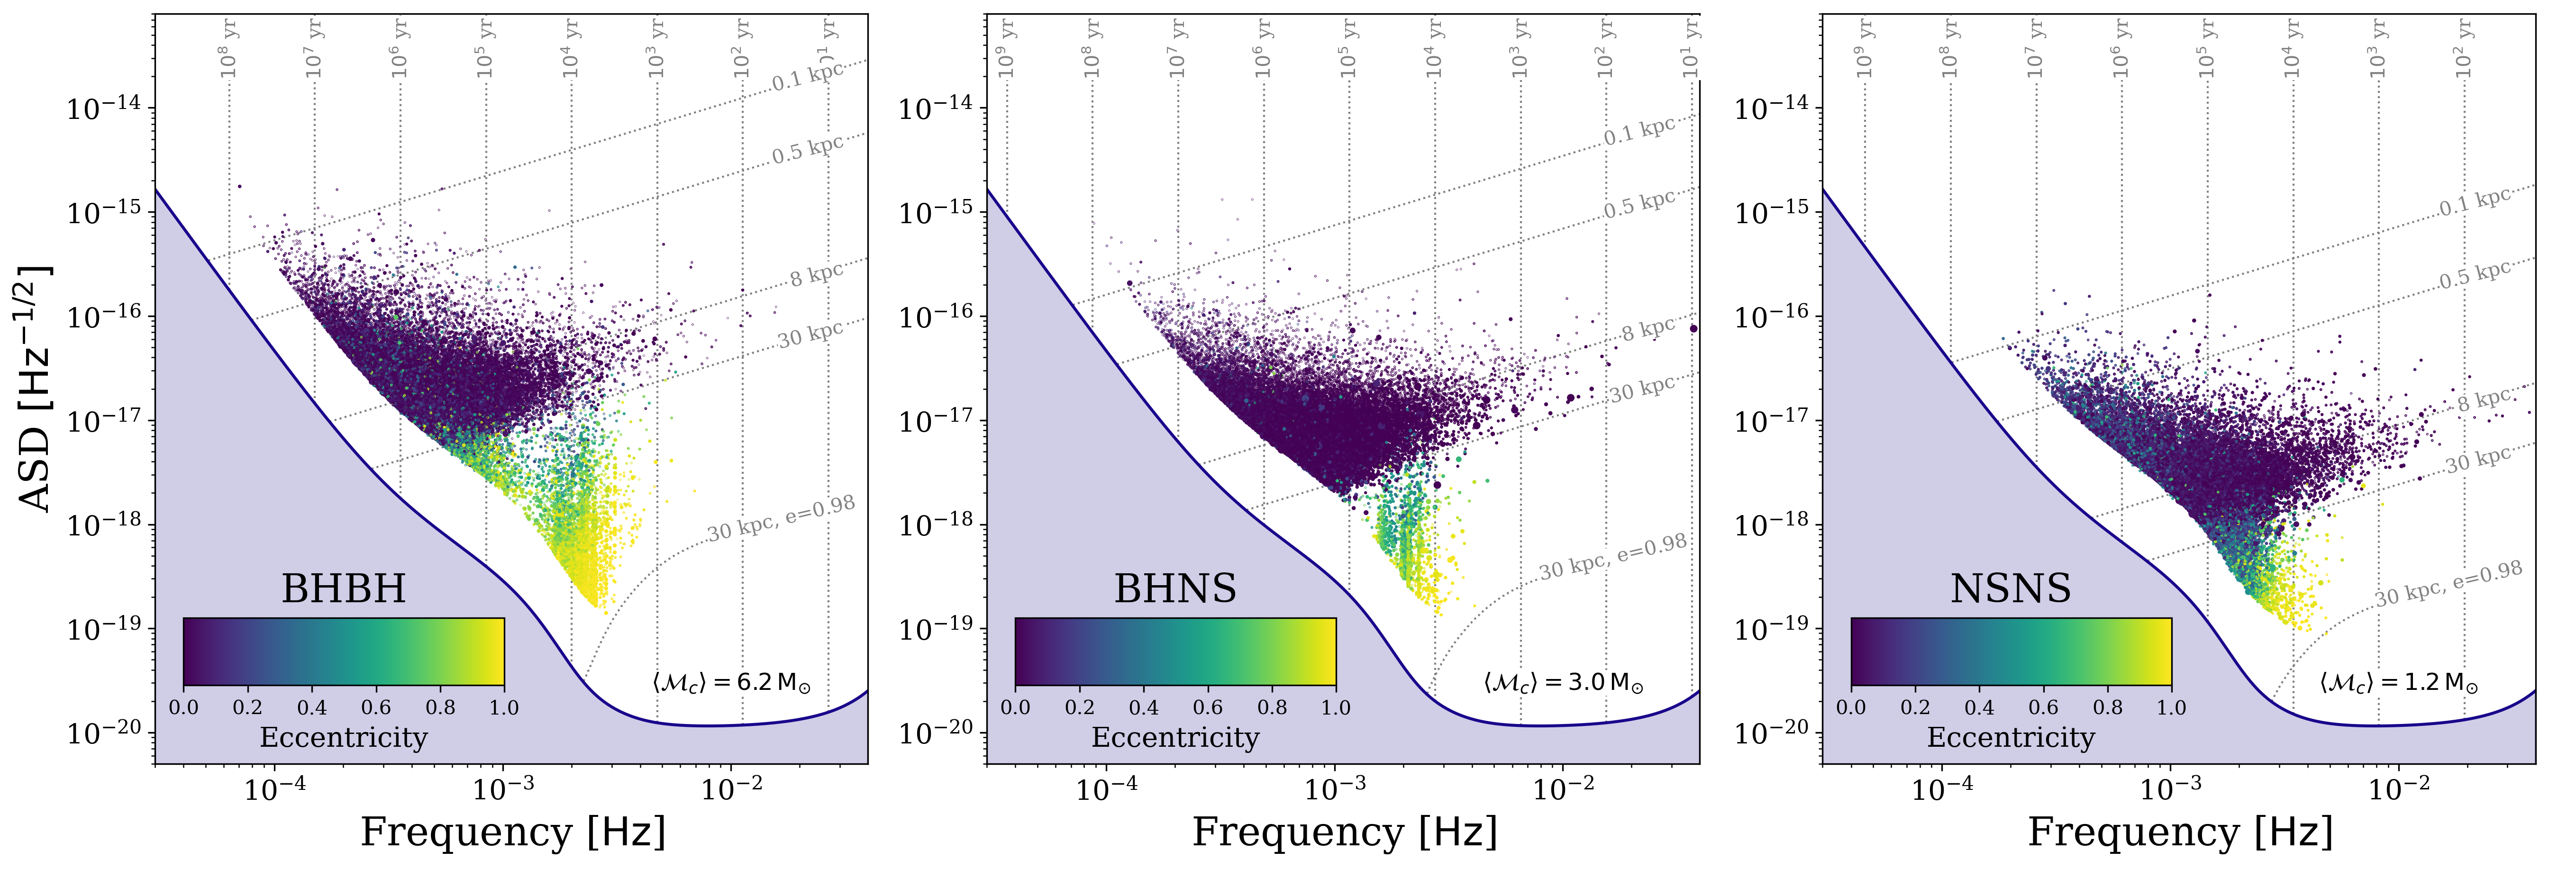
\includegraphics[width=\textwidth]{figF2_dcos_on_sc_eccentric_colours.png}
    \caption{As the bottom panels of Fig.~\ref{fig:dcos_on_sc}, but without the density distributions and scatter points are coloured by their eccentricity. We show eccentric sources are located in an offshoot below the $30 \unit{kpc}$ around $2 \unit{mHz}$. \href{https://github.com/TomWagg/detecting-DCOs-in-LISA/blob/main/paper/figures/figF2_dcos_on_sc_eccentric_colours.png}{\faFileImage} \href{https://github.com/TomWagg/detecting-DCOs-in-LISA/blob/main/paper/figure_notebooks/sensitivity_curve.ipynb}{\faBook}.}
    \label{fig:dcos_on_sc_ecc_col}

    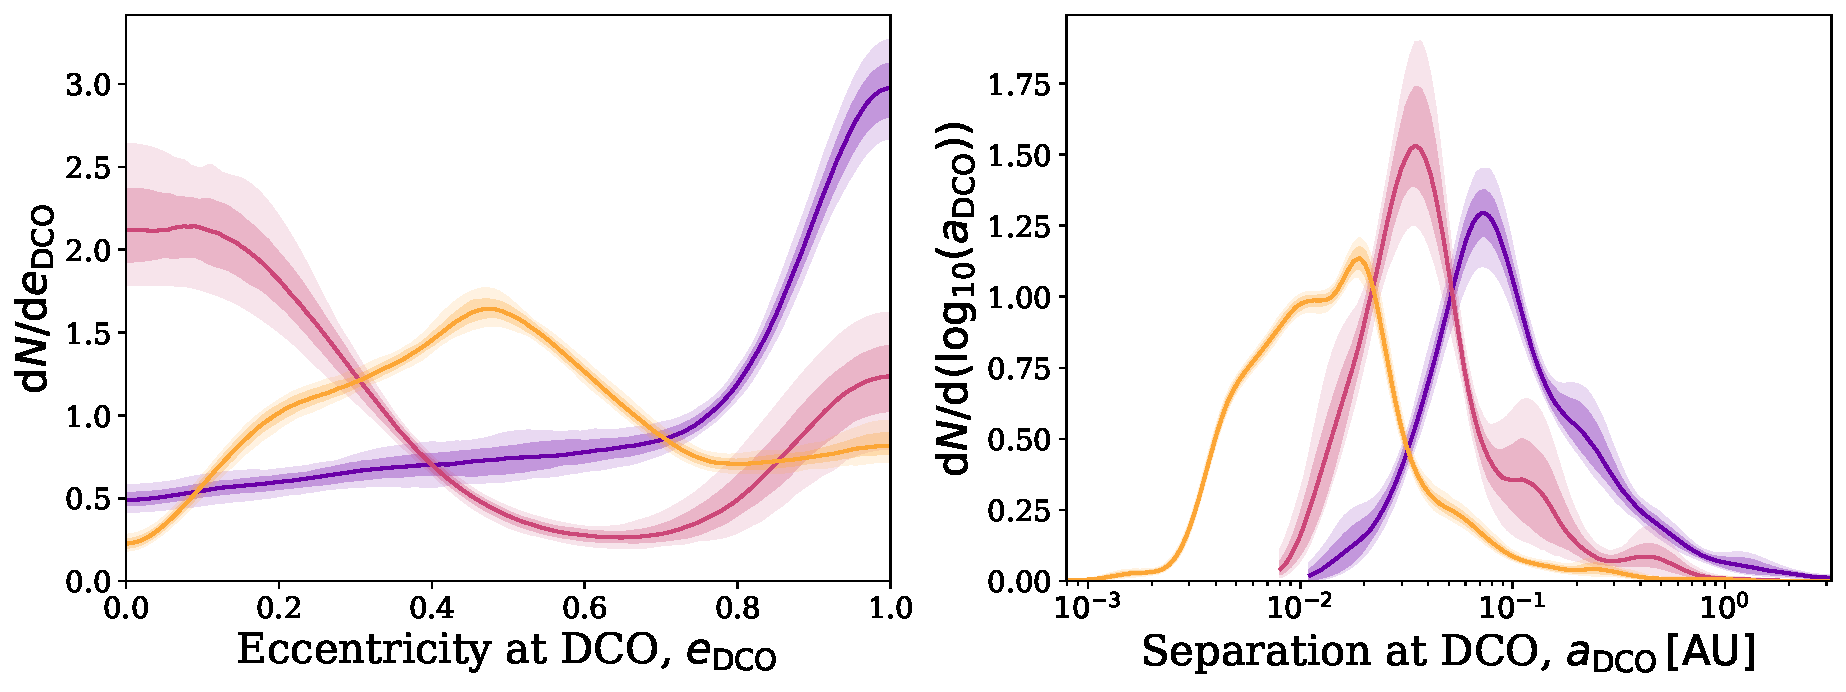
\includegraphics[width=0.8\textwidth]{figF3_dco_formation_distributions.pdf}
    \caption{As Fig.~\ref{fig:fiducial_pdf_distributions}, but for the properties of the detectable systems at DCO formation. \href{https://github.com/TomWagg/detecting-DCOs-in-LISA/blob/main/paper/figures/figF3_dco_formation_distributions.pdf}{\faFileImage} \href{https://github.com/TomWagg/detecting-DCOs-in-LISA/blob/main/paper/figure_notebooks/fiducial.ipynb}{\faBook}.}
    \label{fig:dco_formation_properties}
\end{figure*}


\end{document}
